%160602RR-- HR modification to new (u',v') coordinates completed; results on sporadic rational solutions and closure property added
%160516RR--JCL
%160515RR -- JCL [Revert to old section 8 from 160401.\
%160514 JCL [SUBSECTION TREATING RATIONAL PT ON HYPERBOLA CASE 3 DROPPED AFTE VERSION 160401; SECTIONS RESTRED HERE
% WITH REDUNDANCY[
%160513  JCL [Rearrange sections]
%160511 HR [section 4 divided into 4 and 7, definition of third quadrant residual sets adjusted (same outcome),] 
%160420 new definition of (u',v') coordinates, more changes / additions to section 5, subsection 2.3 added 
%160409 section 5 reworked
%160404 figures 3 and 11 fixed
%160403
%160402 Prop. 5.12
%160401a merge with Richman
%160401 sect 5
%160328 fraenkel refs.
%160324 Macros \uu and \vv added to allow the coordinate system in section 5 to have a different notation than that in section 4
%160322 Revised Sec 1.2; Revised Lemma 5.3 statement; Revised Proposition 5.12 [proof must be further corrected]
%160321 Revised section 4 to exclude sporadic solutions. Restated Prop. 3.1, proved it at end of section 4
% 160321[Section 5 remains to be debugged similarly, Prop. 3.2 restated, and missing proofs found.]
%160301
%160229, version b
%160229 Prop 3.2 proof, sect 5.7
%160228 debug Prop. 3.2+proof, debug section 5.
%160227 Prop 3.1 + proofs; debug Section 4
%160226 [commutators-new title], Lemma 4.13 revised, many small changes
%160225 [Revising section 4.4. [It is a mess now, and needs editing]
% 160224 restate Thm. 4.9, Delete conjecture 4.16. 
% (Delete material after end of paper)
%160223 Lemma 5.3 revised [Richman + JCL]
%160222 Frobenius problem update
%160221 sporadic rational points lemmas 4.15 and 5.12; references; revised Prop. 3.1.
% [Lemma 4.15 and Lemma 4.14 should be combined into one lemma in next draft]
%160220
%160219b
%160219  rewrote lemma 4.10 , changed statement; new proof added-- Lemma 5.11 (rationals on hyperbolas)
%160218 Lemma 5.9 shortened, proof of Thm (ii-b) in section 3 added
%160217 Lemma 5.11 continuing fill in/ number change to Lemma 5.10.
%160216 Lemma 5.11 started filling in
%160215 [fix Lemma 5.9, changed answer Main Thm (iii-c).; debug Prop. 2.6 statement
%160214, version a; compressed Main Thm 3-rd quadrant cases for parallelism with 1-st quadrant
%160214 The u is rational case started: new lemmas 5.11, 5.12 formulated;  split sect 5 into several new subsections, flowchart given in  new section 5.2
%160213a correct case 9iii-c)
%160213 ne lemma 5.8, 5.9
%160212 new Section 2.3 [Harry]
%160211 new Lemma 5.2 [before 5.3
%160210a
%160210 new Lemma 5.4 
%160209 
%160208 corrected lemma 2.3 statement; corrected sign in third quadrant uv coord in sec. 3.2 
%160207b
%160207
%160206 revised proof of Lemma 4.12; new lemma 4.15 added
%160205 third quadrant case lemma 5.2, lemma 5.3
%160204b new theorem 4.9 added [missing proof]
%160204a
%160204
%160203; new lemma 4.3 added, old Lemma 4.10
%160202Skolem; sec 3. [Stuff after end of file is removed.]

%160127
%160126

%160125a
%160124

%160122 rounding back out of appendix
%160121 rounding to appendix

%16019
%160118shrt



\documentclass[12pt,letterpaper, reqno]{amsart}

\usepackage{times}
\usepackage[T1]{fontenc}
\usepackage{mathrsfs, enumerate}
\usepackage{latexsym}
%\usepackage[dvips]{graphics}
%\usepackage{epsfig, tikz}
\usepackage{tikz}
\usetikzlibrary{decorations.pathreplacing}
\usepackage{amsmath,amsfonts,amsthm,amssymb,amscd,mathtools}

%%%%%%%%%%%%%%%
%for correct figure numbering
\usepackage{chngcntr}
%\counterwithout{figure}{section} %continuous numbering
\counterwithin{figure}{section} %by-section numbering
%%%%%%%%%%%%%%%%%%%%


%\input amssym.def
%\input amssym.tex
%\usepackage{showkeys}

% Theorem / Lemmas et cetera

\newtheorem{thm}{Theorem}[section]
\newtheorem{conj}[thm]{Conjecture}
\newtheorem{cor}[thm]{Corollary}
\newtheorem{lem}[thm]{Lemma}
\newtheorem{prop}[thm]{Proposition}
\newtheorem{exe}[thm]{Exercise}
\newtheorem{cla}[thm]{Claim}

\theoremstyle{definition}
\newtheorem{defi}[thm]{Definition}

\theoremstyle{remark}
\newtheorem{rmk}[thm]{Remark}
\newtheorem{exa}[thm]{Example}
\newtheorem{que}[thm]{Question}
\newtheorem{prob}{Problem}
% General Symbols

\def\notdiv{\ \mathbin{\mkern-8mu|\!\!\!\smallsetminus}}

%Blackboard Letters

\newcommand{\sgn}{{\rm sgn}}
\newcommand{\RR}{\ensuremath{\mathbb{R}}}
\newcommand{\CC}{\ensuremath{\mathbb{C}}}
\newcommand{\ZZ}{\ensuremath{\mathbb{Z}}}
\newcommand{\QQ}{\mathbb{Q}}
\newcommand{\NN}{\mathbb{N}}
\newcommand{\FF}{\mathbb{F}}
\newcommand{\TT}{\mathbb{T}}
\newcommand{\WW}{\mathbb{W}}
\renewcommand{\AA}{\mathbb{A}}
\newcommand{\PP}{\mathbb{P}}

%%%%%%%%%%%%%
% new coordinates
%%%%%%%%%%%%%
\newcommand{\uu}{{u'}}
\newcommand{\vv}{{v'}}
\newcommand{\ww}{w}
\newcommand{\uuu}{u_2}
\newcommand{\vvv}{v_2}

\newcommand{\R}{{R}}
\newcommand{\sB}{{\mathcal B}}
\newcommand{\sL}{{\mathcal L}}
\newcommand{\bv}{{\bf v}}
\newcommand{\bbv}{{\bf v}^{'}}
\newcommand{\sO}{{\mathcal O}}
%\newcommand{\Qoft}{\mathbb{Q}(t)}  %use in linux
\newcommand{\floor}[1]{\lfloor{#1}\rfloor}
\newcommand{\bfloor}[1]{\bigg\lfloor{#1}\bigg\rfloor}
\newcommand{\ceil}[1]{\lceil{#1}\rceil}
\newcommand{\bceil}[1]{\bigg\lceil{#1}\bigg\rceil}

%%%%%%%%
% Rounding function 2
\newcommand{\tround}{\vec{r}}
\newcommand{\round}{r}
%%%%%%%%

\DeclareMathOperator{\Cond}{Cond}
\DeclareMathOperator{\cond}{cond}
\DeclareMathOperator{\Int}{Int}
\DeclareMathOperator{\covol}{covol}
%\DeclareMathOperator{\int}{int}
\DeclareMathOperator{\lcm}{lcm}

\newcommand{\mattwo}[4]
{\left(\begin{array}{cc}
                        #1  & #2   \\
                        #3 &  #4
                          \end{array}\right) }

\newcommand{\vertvectwo}[2]
{\left(\begin{array}{c}
                    #1 \\
                    #2
                    \end{array}\right) }

\paperheight=11in
\paperwidth=8.5in


\setlength{\marginparwidth}{30pt}
\setlength{\oddsidemargin}{0pt}
\setlength{\evensidemargin}{0pt}
\setlength{\textwidth}{450pt}
\setlength{\voffset}{0pt}
\setlength{\topmargin}{0pt}
\setlength{\textheight}{650pt}

\newcommand{\abs}[1]{\left|#1\right|}

%%%%%make-equation-numbers-by-section%%%%%%%
\renewcommand{\theequation}{\arabic{section}.\arabic{equation}}
%%%%%%%%%%%%%%%%%%%%%%%%%%%

%%%%%%
% TITLE
%%%%%%
\title{ Commutator inequalities for dilated floor functions}

\author{Jeffrey C. Lagarias}
\author{David Harry Richman}
\address{Dept.\ of Mathematics, University of Michigan,
Ann Arbor, MI 48109--1043}
\email{lagarias@umich.edu}
\email{hrichman@umich.edu}


\subjclass[2010]{ 26D07 (primary), 39B72 (secondary)}
\date{May 16, 2016RR. Preliminary draft, not debugged, not for circulation.}
\begin{document}

\maketitle

\bibliographystyle{amsplain}


%%%%%%%%%%%%%%%%%%%%%%%%%%%%%%%%%%%%%%%%%%%%%%%%%%%%%%%%%%%%%%%%%%%%%%%%%%%%%%%%%%%%%%%%
%
% section 1: INTRODUCTION
%
%%%%%%%%%%%%%%%%%%%%%%%%%%%%%%%%%%%%%%%%%%%%%%%%%%%%%%%%%%%%%%%%%%%%%%%%%%%%%%%%%%%%%
\section{Introduction}
The {\em floor function}  
$\lfloor x \rfloor$
rounds a real number down to the nearest integer. 
Given a real parameter $\alpha$, we may define the {\em dilated} floor function $f_\alpha(x)= \floor{\alpha x}$.
The behavior of these functions is easy to understand, 
i.e. $f_\alpha$ is the sum of a linear function and a piecewise-linear periodic function, but the composition of two such functions 
$ f_{\alpha,\beta}(x) = \floor{\alpha \floor{\beta x}}$
exhibits more subtle behavior. In general they do not commute under composition.
A number of identities relating dilated floor functions with different dilation factors are given in 
Graham, Knuth and Patashnik \cite[Chap. 3]{GKP94}.
They raised problems  \cite[Research problem 50, p.101]{GKP94}
concerning compositions of dilated floor functions, some later addressed in  Graham and O'Bryant \cite{Go10}. 

Recently the  authors together with T. Murayama \cite{LMR16}  
gave necessary and sufficient conditions on $(\alpha, \beta)$ 
for these functions to commute 
under composition, i.e. determining when
 $\floor{\alpha \floor{\beta x}} =  \floor{\beta \floor{\alpha  x}}$ 
 holds for all $x \in \RR.$  Examples of commuting compositions of dilated floor functions
 were noted  in 2010 by  Cardinal \cite[Lemma 6]{Car10} in  a number-theoretic context.

% This paper  considers a more general question
The commutator 
$$
 [ f_{\alpha}, f_{\beta}](x) := f_{\alpha, \beta} (x) - f_{\beta, \alpha}(x)= \floor{\alpha \floor{\beta x}} -  \floor{\beta \floor{\alpha  x}}
$$ 
is a bounded generalized polynomial in
the sense of Bergelson and Leibman \cite{BerL07}. 
We address the problem of determining the parameters $(\alpha, \beta)$ for which  the one-sided inequality \begin{equation}\label{ineq}
\floor{\alpha \floor{\beta x}} -  \floor{\beta \floor{\alpha  x}} \ge 0 \quad \text{for all} \quad  x \in \RR
\end{equation}
holds.
% for such commutators. 



%%%%%%%%%%%%%%%%%%%%%%%%%%%%%%%%%%%%%%%%%%%%%%%%%%%%%%%%%%%%%%%%%%%%%%%%%%%%%%%%%%%%%%%%%%%%%
%  Section 1.1 MAIN RESULT inequality Case
%
%%%%%%%%%%%%%%%%%%%%%%%%%%%%%%%%%%%%%%%%%%%%%%%%%%%%%%%%%%%%%%%%%%%%%%%%%%%%%%%%%%%%%%%%%%%%%
\subsection{Main Result}

Our main result gives a  classification of the parameters $(\alpha, \beta)$
satisfying the inequality \eqref{ineq}.  % Inequality Case}

%%%%%%%%%%%%%%%%%%%%%%%%%%%%%%%%%%
%
% Main Theorem 1.1
%
%%%%%%%%%%%%%%%%%%%%%%%%%%%%%%%%%%
\begin{thm} \label{thm:main}
The parameters  $(\alpha, \beta) \in \RR^2$  that satisfy the inequality
$$\lfloor \alpha \lfloor \beta x\rfloor \rfloor \geq \lfloor \beta \lfloor \alpha x\rfloor \rfloor
\quad \mbox{for all} \quad x \in \RR
$$
 consist of the two coordinate axes $\{(\alpha, 0): \alpha  \in \RR \}$
and $\{ (0, \beta):  \beta \in \RR\}$ together with  the following points. 
\begin{enumerate}
\item[(i)] 
{\rm (First Quadrant)} These points with  $\alpha>0$ and $\beta >0$ that satisfy
the inequality  fall into three collections of one-parameter continuous families.
\begin{enumerate}
\item[(i-a)] For each integer $m_1 \ge 1$ all points with $\alpha >0$ that lie on the line $\beta= m_1 \alpha$ of slope $m_1$ through the origin,
i.e. $\{ (\alpha, m_1 \alpha): \, \alpha >0\}$.
\item[(i-b)] For each  integer $m_2 \ge 1$ all points with $\beta >0$ that lie on the  vertical line $\alpha= \frac{1}{m_2}$ i.e. 
$\{(\frac{1}{m_2}, \beta): \, \beta >0 \}$.
\item[(i-c)] For each pair of integers $m_1\ge 1$ and $m_2 \ge 1$, all points with $\beta>0$ that lie on the 
rectangular hyperbola
$$m_1 \alpha \beta + m_2 \alpha - \beta =0.$$
%\item[(i-d)] Possible  sporadic rational solutions $(\alpha, \beta) \in \QQ^2$.  Any that  exist must satisfy $0 < \alpha <\max \{ \beta, 1\}$.
%[NOT YET ANALYZED]
\end{enumerate} 
\item[(ii)] {\rm (Second quadrant)} All points with $\alpha <0$ and $\beta >0$ satisfy the inequality.
\item[(iii)] {\rm (Third quadrant)} All points with $\alpha <0$ and $\beta <0$ that satisfy the inequality
have $|\alpha| \ge |\beta|$. They fall into three collections of one parameter continuous families, plus
additional sporadic rational solutions. 
\begin{enumerate}
\item[(iii-a)] For each integer $ m_1 \ge 1$ all points with $\alpha <0$ that lie on the line $\alpha=m_1\beta$
of slope $\frac{1}{m_1}$ through the origin,
i.e. $\{ (\alpha,  \frac{1}{m_1} \alpha): \, \alpha <0\}$.
\item[(iii-b)] For each positive rational $\frac{m_1}{m_2}$ given in lowest terms,
all points  $(-\frac{m_1}{m_2} , -\beta)$ that lie on the 
vertical  line segment  $0 <\beta \le \frac{1}{m_2}$.
%$\alpha= -\frac{m_1}{m_2}$, for the range   $-\frac{1}{m_2} \le \beta < 0$.
\item[(iii-b')] Sporadic rational solutions $(\alpha, \beta) \in \QQ^2$. These include  an infinite set
 $(\alpha, \beta) = (-m_1, -\frac{m_1 r}{m_1r -j}),$ parametrized by integers $(m_1, j, r )$ with  $m_1 \ge 2$,  $1 \le j \le m_1 -1$, and $r \ge 1$.
 which comprise all sporadic solutions having $ \beta < -1.$
\item[(iii-c)]
For  each pair of integers $m_1 \ge 1$ and $m_2 \ge 1$, all  points having $\alpha <0$  that  lie on the 
rectangular hyperbola $\,\,$ 
$$m_1\alpha \beta   + \alpha- m_2\beta =0.$$
%There are infinitely many of them, and
%Any  further sporadic rational  solutions that exist must have $-1\le  \beta<0$. 
 %[NOT YET ANALYZED]
\end{enumerate} 
\item[(iv)] {\rm (Fourth quadrant)} No point with $\alpha >0$ and $\beta <0$ satisfies the inequality.

\end{enumerate}
\end{thm}

A {\em sporadic rational solution} is  a rational solution that does not lie
on any of the one-parameter families of solutions given above. 
These are solutions  $(\alpha, \beta) \in \QQ^2$ of \eqref{ineq} which are not  limit 
points of other solutions that  have at least one  irrational parameter. 
An interesting part of the proof  of Theorem \ref{thm:main}  is that of ruling out any
sporadic rational solutions in the first quadrant case. This question is related to the
Diophantine Frobenius problem in two dimensions.
There exist infinitely many sporadic rational solutions in the third quadrant, having $|\beta|> 1$.
We have not (yet) classified the sporadic rational solutions in the third quadrant having $-1 \le \beta <0$
but there are many in this region. In Proposition \ref{prop:sporadic-rational} we give a testable criterion for such solutions,
showing they have a restricted form. 
%An analysis ruling out any sporadic rational  solutions having $|\beta| \le 1$ in the third quadrant case again involves a similar analysis to the first quadrant case. 


An  interesting feature of the answer is the  internal structures of the parametric families of solutions in
the first quadrant 
%(case (i)) 
and the third quadrant. These consist of straight lines and arcs of rectangular hyperbolas.
%(case (iii)).
Straight lines occur  in the equality case, but a new feature here 
 is the occurrence of families of arcs of rectangular hyperbolas  in
case {\it (i-c)} and case {\it (iii-c)}, respectively. These arcs of hyperbolas all pass through the origin.
Some of the  hyperbolas in case {\it (iii-c)} are continuations of the arcs of hyperbolas
in case {\it (i-c)}; these occur exactly when the parameter $m_2=1$ in the two cases,
as is apparent from their given equations. 
Figure \ref{fig1} gives a
plot of these solutions in the first and third quadrants.

%%%%%%%%%%%%%%%%%%%%%%%%%%%%%%%%%%%%%%%%%%%%%%%%%%%%%%%%%%%%%%%%%%%%%%%%%%%%%%%%%%%
%
% Figure 1  Solutions in (\alpha, \beta)-coordinates
%%%%%%%%%%%%%%%%%%%%%%%%%%%%%%%%%%%%%%%%%%%%%%%%%%%%%%%%%%%%%%%%%%%%%%%%%%%%%%%%%%%
\begin{figure}[h]
\begin{center}
\begin{tikzpicture}[scale=.6]
  \draw[->] (-8,0) -- (8,0) node[right] {$\alpha$};
  \draw[->] (0,-8) -- (0,8) node[above] {$\beta$};
  \draw[scale=4] (1,0.05) -- (1,-0.05) node[below] {1};
  \draw[scale=4] (0.05,1) -- (-0.05,1) node[left] {1};
  
  \fill[scale=4,gray,nearly transparent] (0,0) -- (0,1.9) -- (-1.9,1.9) -- (-1.9,0) -- cycle;
  
  \draw[xscale=4,yscale=4,domain=-1.9:1.9,smooth,variable=\x, blue] plot ({\x},{\x});
  \draw[xscale=4,yscale=4,domain=0:1.9,smooth,variable=\x, blue] plot ({\x/2},{\x});
  \draw[xscale=4,yscale=4,domain=0:1.9,smooth,variable=\x, blue] plot ({\x/3},{\x});
  \draw[xscale=4,yscale=4,domain=0:1.9,smooth,variable=\x, blue] plot ({\x/4},{\x});
  \draw[xscale=4,yscale=4,domain=0:1.9,smooth,variable=\x, blue] plot ({\x/5},{\x});
  \draw[xscale=4,yscale=4,domain=0:1.9,smooth,variable=\x, blue] plot ({\x/6},{\x});
  \draw[xscale=4,yscale=4,domain=0:1.9,smooth,variable=\x, blue] plot ({\x/7},{\x});
  \draw[xscale=4,yscale=4,domain=0:1.9,smooth,variable=\x, blue] plot ({\x/8},{\x});
  
  \draw[xscale=4,yscale=4,domain=-1.9:0,smooth,variable=\x, blue] plot ({\x},{\x/2});
  \draw[xscale=4,yscale=4,domain=-1.9:0,smooth,variable=\x, blue] plot ({\x},{\x/3});
  \draw[xscale=4,yscale=4,domain=-1.9:0,smooth,variable=\x, blue] plot ({\x},{\x/4});
  \draw[xscale=4,yscale=4,domain=-1.9:0,smooth,variable=\x, blue] plot ({\x},{\x/5});
  \draw[xscale=4,yscale=4,domain=-1.9:0,smooth,variable=\x, blue] plot ({\x},{\x/6});
  \draw[xscale=4,yscale=4,domain=-1.9:0,smooth,variable=\x, blue] plot ({\x},{\x/7});
  \draw[xscale=4,yscale=4,domain=-1.9:0,smooth,variable=\x, blue] plot ({\x},{\x/8});
  
  \draw[xscale=4,yscale=4,domain=0:1.9,smooth,variable=\y, red]  plot ({1},{\y});
  \draw[xscale=4,yscale=4,domain=0:1.9,smooth,variable=\y, red]  plot ({1/2},{\y});
  \draw[xscale=4,yscale=4,domain=0:1.9,smooth,variable=\y, red]  plot ({1/3},{\y});
  \draw[xscale=4,yscale=4,domain=0:1.9,smooth,variable=\y, red]  plot ({1/4},{\y});
  \draw[xscale=4,yscale=4,domain=0:1.9,smooth,variable=\y, red]  plot ({1/5},{\y});
  \draw[xscale=4,yscale=4,domain=0:1.9,smooth,variable=\y, red]  plot ({1/6},{\y});
  \draw[xscale=4,yscale=4,domain=0:1.9,smooth,variable=\y, red]  plot ({1/7},{\y});
  \draw[xscale=4,yscale=4,domain=0:1.9,smooth,variable=\y, red]  plot ({1/8},{\y});
  
  \draw[xscale=4,yscale=4,domain=-1:0,smooth,variable=\y, red]  plot ({-1},{\y});
  \draw[xscale=4,yscale=4,domain=-1/2:0,smooth,variable=\y, red]  plot ({-1/2},{\y});
  \draw[xscale=4,yscale=4,domain=-1/2:0,smooth,variable=\y, red]  plot ({-3/2},{\y});
  \draw[xscale=4,yscale=4,domain=-1/3:0,smooth,variable=\y, red]  plot ({-1/3},{\y});
  \draw[xscale=4,yscale=4,domain=-1/3:0,smooth,variable=\y, red]  plot ({-2/3},{\y});
  \draw[xscale=4,yscale=4,domain=-1/3:0,smooth,variable=\y, red]  plot ({-4/3},{\y});
  \draw[xscale=4,yscale=4,domain=-1/3:0,smooth,variable=\y, red]  plot ({-5/3},{\y});
  \draw[xscale=4,yscale=4,domain=-1/4:0,smooth,variable=\y, red]  plot ({-1/4},{\y});
  \draw[xscale=4,yscale=4,domain=-1/4:0,smooth,variable=\y, red]  plot ({-3/4},{\y});
  \draw[xscale=4,yscale=4,domain=-1/4:0,smooth,variable=\y, red]  plot ({-5/4},{\y});
  \draw[xscale=4,yscale=4,domain=-1/4:0,smooth,variable=\y, red]  plot ({-7/4},{\y});
  \draw[xscale=4,yscale=4,domain=-1/5:0,smooth,variable=\y, red]  plot ({-1/5},{\y});
  \draw[xscale=4,yscale=4,domain=-1/5:0,smooth,variable=\y, red]  plot ({-2/5},{\y});
  \draw[xscale=4,yscale=4,domain=-1/5:0,smooth,variable=\y, red]  plot ({-3/5},{\y});
  \draw[xscale=4,yscale=4,domain=-1/5:0,smooth,variable=\y, red]  plot ({-4/5},{\y});
  \draw[xscale=4,yscale=4,domain=-1/5:0,smooth,variable=\y, red]  plot ({-6/5},{\y});
  \draw[xscale=4,yscale=4,domain=-1/5:0,smooth,variable=\y, red]  plot ({-7/5},{\y});
  \draw[xscale=4,yscale=4,domain=-1/5:0,smooth,variable=\y, red]  plot ({-8/5},{\y});
  \draw[xscale=4,yscale=4,domain=-1/6:0,smooth,variable=\y, red]  plot ({-1/6},{\y});
  \draw[xscale=4,yscale=4,domain=-1/7:0,smooth,variable=\y, red]  plot ({-1/7},{\y});
  \draw[xscale=4,yscale=4,domain=-1/8:0,smooth,variable=\y, red]  plot ({-1/8},{\y});
  % sporadic solutions
  \foreach \y in {6/10,9/16,12/22}{% node on the grid we have drawn 
    \node[draw,circle,inner sep=0.5pt,fill,red] at (-3/2*4,-1*\y*4) {};  }
  \foreach \y in {9/14,12/20}{% node on the grid we have drawn 
    \node[draw,circle,inner sep=0.5pt,fill,red] at (-3/2*4,-1*\y*4) {};  }
  \foreach \y in {4/9,6/15,8/21,10/27}{% node on the grid we have drawn 
    \node[draw,circle,inner sep=0.5pt,fill,red] at (-2/3*4,-1*\y*4) {};  }
  \foreach \y in {4/9,6/15,8/21,10/27}{% node on the grid we have drawn 
    \node[draw,circle,inner sep=0.5pt,fill,red] at (-4/3*4,-1*\y*4) {};  }
  \foreach \y in {4/9,6/15,8/21,10/27}{% node on the grid we have drawn 
    \node[draw,circle,inner sep=0.5pt,fill,red] at (-5/3*4,-1*\y*4) {};  }
  
  \draw[xscale=4,yscale=4,domain=-1.9:.655,smooth,variable=\x, green] plot ({\x},{\x/(1-\x)});
  \draw[xscale=4,yscale=4,domain=-1.9:.4,smooth,variable=\x, green] plot ({\x},{\x/(1-2*\x)});
  \draw[xscale=4,yscale=4,domain=-1.9:.285,smooth,variable=\x, green] plot ({\x},{\x/(1-3*\x)});
  \draw[xscale=4,yscale=4,domain=0:.5,   smooth,variable=\x, green] plot ({\x},{2*\x/(1-\x)}); %1st quadrant
  \draw[xscale=4,yscale=4,domain=-1.9:0,smooth,variable=\x, green] plot ({\x},{\x/(2-\x)}); %3rd quadrant
  
\end{tikzpicture}
\end{center}
\caption{Solutions to \eqref{ineq}   first and third quadrants of the $(\alpha,\beta)$-plane}
\end{figure} \label{fig1}



%%%%%%%%%%%%%%%%%%%%%%%%%%%%%%%%%%%%%%%%%%%%%%%%%%%%%%%%%%%%%%%%%%%
%
%  Section 1.2 Equality Case
%
%%%%%%%%%%%%%%%%%%%%%%%%%%%%%%%%%%%%%%%%%%%%%%%%%%%%%%%%%%%%%%%%%%%
\subsection{Equality case}
%An immediate corollary of Theorem \ref{thm:main} is 

We recall the classification of the case of equality,
which has a simple direct proof 
given in \cite{LMR16}.

%%%%%%
%
% Theorem 1.2
%
%%%%%%
\begin{thm} \label{thm:main-eq}
  The complete set of all $(\alpha, \beta) \in \RR^2$ such that
  \[
    \lfloor \alpha \lfloor \beta x\rfloor \rfloor
    = \lfloor \beta \lfloor \alpha x\rfloor \rfloor
  \]
  holds for all $x \in \RR$ consists of:
  \begin{enumerate}
    \item[(i)]
      Three one-parameter continuous families $(\alpha, \alpha)$, $(\alpha, 0)$, $(0, \alpha)$ for
      all $\alpha \in \RR$. 
    \item[(ii)]
      The infinite discrete family 
      \[
        \left\{ (\alpha, \beta) = \left(\frac{1}{m}, \frac{1}{n}\right) : m, n
        \ge 1 \right\},
      \]
      where $m,n$ are positive integers. (The continuous and discrete families overlap when $m=n$.) 
  \end{enumerate}
\end{thm}

To see that Theorem \ref{thm:main-eq}  follows  from Theorem \ref{thm:main}
we intersect the solution set of  Theorem \ref{thm:main} with
a  copy of it obtained by reflecting around the line $\alpha=\beta$, i.e. exchanging $\alpha$ and $\beta$.
The coordinate axes $\alpha=0$ and $\beta=0$ and the line $\alpha=\beta$ are clearly 
invariant under reflection, so it remains to 
 study this map on the four open quadrants.
 This map interchanges
the second and fourth quadrant and takes the first and third quadrants into themselves,
reflected around the line $\alpha =\beta$.
\begin{enumerate}
\item
The intersection of the solutions in Theorem \ref{thm:main} in the open second quadrant
and open fourth quadrant is clearly the empty set. 
\item
The intersection of solutions in 
Theorem \ref{thm:main} in the third quadrant under the reflection includes  the line $\alpha=\beta$.
This intersection is exactly this line, 
because Theorem \ref{thm:main} states there are no solutions having $|\beta| > |\alpha|$.
\item 
Finally the intersections in the first quadrant certainly includes the invariant line $\alpha=\beta$,
which is $m_1=1$ in case {\it (i-a)}. 
%otherwise are pairwise intersections of lines and hyperbolas under the reflection operation.
We next note that there are no solutions in this quadrant having $\alpha > \beta$
aside from  those coming from the case {\it (i-b)} vertical line solutions $\alpha= \frac{1}{m_1}$
for $m_1 \ge 1$. Since the solution set must be invariant under exchange of variables,
the second coordinate must be of the form $\beta =\frac{1}{m_2}$ for some integer $m_2 \ge 1$
as well. But all such points $(\frac{1}{m_1}, \frac{1}{m_2})$ lie in the solution set and its
reflection (which have horizontal lines $\beta= \frac{1}{m_2}$.)
 %remaining solutions are of the form $(\frac{1}{m_1}, *).$ [TBA]
\end{enumerate}

A proof of Theorem \ref{thm:main-eq} via Theorem \ref{thm:main} is roundabout, in
that the latter proof requires the exclusion of sporadic rational solutions in the first
quadrant, which is  complicated in the proof given here.
%One checks that  every such intersection is empty or else is a point of form $(\frac{1}{m_1}, \frac{1}{m_2})$
%for integers $m_1, m_2 \ge 1$, and that all such points do occur. 


%This result provides a constraint on the structure of sporadic rational solutions. 
%It relates to a two known asymmetries in solutions of the two dimensional Frobenius problem.



%%%%%%%%%%%%%%%%%%%%%%%%%%%%%%%%%%%%%%%%%%%%%%%%%%%%%%%%%%%%%%%%%%%%%%%%%%%%%%%%%%%%%%%%%%%%%
%  Section 1.3 COORDINATE CHANGES AND SYMMETRIES
% 
%%%%%%%%%%%%%%%%%%%%%%%%%%%%%%%%%%%%%%%%%%%%%%%%%%%%%%%%%%%%%%%%%%%%%%%%%%%%%%%%%%%%%%%%%%%%%
\subsection{Coordinate Changes and Symmetries}

We use two  birational  coordinate changes that  simplify the analysis and also reveal
symmetries of the solution set.

%%%%%%%%%%%%%%%%%%%%%%%%%%%%%%%%%%%%%%%%%%%%%%%%%%%%%%%%%%%%%%%%%%%%%%%%%%%%%%
%
%  Section 1.3.1 Birational Change to (u, v) coordinates
%
%%%%%%%%%%%%%%%%%%%%%%%%%%%%%%%%%%%%%%%%%%%%%%%%%%%%%%%%%%%%%%%%%%%%%%%%%%%%%%
\subsubsection{Birational Coordinate Changes to $(u, v)$-coordinates  and $(\uu, \vv)$-coordinates}\label{sec:131}

For the first quadrant case  of $(\alpha, \beta)$ in Theorem \ref{thm:main},  the set of solutions to \eqref{ineq} is 
simpler to analyze after making  the 
coordinate change
from $(\alpha, \beta)$ to new coordinate variables $(u,v)$ via  
$$u := \frac{1}{\alpha}, \quad v  := \frac{\beta}{\alpha}.$$
This is a birational transformation that maps the open first quadrant onto  itself, having  inverse map
$\alpha= \frac{1}{u}, \quad \beta= \frac{v}{u}.$
 Viewed in  the first quadrant of the $(u, v)$-plane 
the classification of Theorem \ref{thm:main} becomes:
\begin{enumerate}
\item[{\it (i-a)}] For each integer $m_1 \ge 1$ all points $(u, v)$ that lie  on the vertical line $u=m_1$, i.e. 
$\{(m_1, v): \, v >0 \}$.
\item[{\it (i-b)}] For each  integer $m_2 \ge 1$ all points $(u, v)$ that lie on the  horizontal line $v= m_2$, i.e. $\{(u, m_2): \, u >0 \}$.
\item[{\it (i-c)}] For each pair of integers $m_1\ge 1$ and $m_2 \ge 1$, all points $(u, v)$ with $u, v>0$ that lie on the rectangular hyperbola
$$\frac{m_1}{u}  + \frac{m_2 }{v} =1.$$
\end{enumerate} 
In the $(u, v)$-coordinate system there is a visible connection of the hyperbola solutions in  the case {\it (i-c)}  to (generalizations of) Beatty sequences. 
The $(u,v)$-coordinate system also reveals a hidden symmetry of  first quadrant solutions:
it is  symmetrical around the line $u= v$.

The third quadrant case  of $(\alpha, \beta)$ can be  analyzed similarly using  a related birational coordinate change, 
taking $(\alpha, \beta)$ to $(\uu, \vv)$ with  
$$\uu := -\frac{1}{\beta}, \quad  \vv := \frac{\alpha}{\beta}.$$ 
This map sends  the  (open) third quadrant onto the (open) first quadrant, and has inverse map
$\alpha= -\frac{\vv}{\uu}, \quad \beta= -\frac{1}{\uu}.$
 The classification of Theorem \ref{thm:main} viewed in  the first quadrant of the $(\uu, \vv)$-plane  becomes:
\begin{enumerate}
\item[{\it (iii-a)}] For each integer $m_1 \ge 1$ all points $(\uu, \vv)$ that lie  on the horizontal line $\vv={m_1}$, i.e. 
$\{(\uu, {m_1}): \, \uu >0 \}$.

\item[{\it (iii-b)}] For all  integers $m_2, m_3 \ge 1$ all points $(\uu, \vv)$ that lie on the diagonal line  $\vv= \frac{m_2}{m_3}\uu$
with $\uu \ge {m_3}$, i.e. $\{(\uu,\frac{m_2}{m_3}\uu): \,  \uu \geq {m_3} \}$.

\item[\it (iii-b')] For each integer $m_2 \ge 2$ the  sporadic solutions in the parametric family $(\uu, \vv) := (1-\frac{j}{m_2 r}, m_1-\frac{j}{r})$
with parameters  $ 1 \le j \le m_2 -1$ and $ r\ge 2$. 
These solutions have
$0 <\uu < 1$ and  $\vv/\uu =m_2$.

\item[{\it (iii-c)}] For each pair of integers $m_1\ge 1$ and $m_2 \ge 1$, all points $(\uu, \vv)$  with $\uu, \vv>0$ that lie on the rectangular hyperbola
$$\frac{m_1}{\uu}  + \frac{m_2 }{\vv} =1.$$

\end{enumerate} 

The solutions to \eqref{ineq} in these coordinates are pictured in Figures \ref{fig-uv-coords} and \ref{fig-uvprime-coords}.
These various coordinates may be explained as follows: if we consider our initial coordinates $(\alpha,\beta)$ as defining an affine open chart $i_0:\AA^2 \to \PP^2$ sending $(\alpha,\beta)\mapsto [\pm 1:\alpha:\beta] = [x_0:x_1:x_2]$ whose image is $\{x_0\neq 0\}$, then  $(u,v)$ are coordinates for a second standard affine open $\{x_1\neq 0\}$, while $(\uu,\vv)$ are coordinates for a third affine open $\{x_2\neq 0\}$. 

The details of the analysis in the third quadrant case parallel that in the first quadrant case,
but become more complicated.   In  the end we will also relate  case {\it (iii-c)} to 
generalizations of Beatty sequences.

%%%%%%%%%%%%%%%%%%%%%
% Figure 2 (u, v)-=coordinates
%%%%%%%%%%%%%%%%%%%%%
\begin{figure}[h]
\begin{center}
\begin{tikzpicture}[scale=.5]
  \draw[->] (0,0) -- (10,0) node[right] {$u=1/\alpha$};
  \draw[->] (0,0) -- (0,10) node[above] {$v=\beta/\alpha$};
  \draw[scale=1.8] (1,0.1) -- (1,-0.1) node[below] {1};
  \draw[scale=1.8] (0.1,1) -- (-0.1,1) node[left] {1};
  
  \draw[scale=1.8,domain=0:5.2,smooth,variable=\x, blue] plot ({\x},{1});
  \draw[scale=1.8,domain=0:5.2,smooth,variable=\x, blue] plot ({\x},{2});
  \draw[scale=1.8,domain=0:5.2,smooth,variable=\x, blue] plot ({\x},{3});
  \draw[scale=1.8,domain=0:5.2,smooth,variable=\x, blue] plot ({\x},{4});
  \draw[scale=1.8,domain=0:5.2,smooth,variable=\x, blue] plot ({\x},{5});
  \draw[scale=1.8,domain=0:5.2,smooth,variable=\y, red]  plot ({1},{\y});
  \draw[scale=1.8,domain=0:5.2,smooth,variable=\y, red]  plot ({2},{\y});
  \draw[scale=1.8,domain=0:5.2,smooth,variable=\y, red]  plot ({3},{\y});
  \draw[scale=1.8,domain=0:5.2,smooth,variable=\y, red]  plot ({4},{\y});
  \draw[scale=1.8,domain=0:5.2,smooth,variable=\y, red]  plot ({5},{\y});
  \draw[scale=1.8,domain=1.24:5.4,smooth,variable=\x, green] plot ({\x},{\x/(\x-1)});
  \draw[scale=1.8,domain=1.62:5.4,smooth,variable=\x, green] plot ({\x},{2*\x/(\x-1)});
  \draw[scale=1.8,domain=2.47:5.4,smooth,variable=\x, green] plot ({\x},{\x/(\x-2)});
\end{tikzpicture}
\end{center}
\caption{First quadrant solutions
to \eqref{ineq} viewed in $(u, v)$-coordinates, with $u= 1/\alpha$ and $v= \frac{\beta}{\alpha}$}\label{fig-uv-coords}
\end{figure} 

%%%%%%%%%%%%%%%%%%%%%%%%%%%%%%%%%%%%%%%%%%%%%%%%%%%%%%%%%%%%%%%%%%%%%%%%%%%%%%%%%%%
% Figure 3 (u', v') coordinates. quadrant 3 
%%%%%%%%%%%%%%%%%%%%%%%%%%%%%%%%%%%%%%%%%%%%%%%%%%%%%%%%%%%%%%%%%%%%%%%%%%%%%%%%%%%
\begin{figure}[h]
\begin{center}
  \begin{tikzpicture}[scale=.5]
  \draw[->] (0,0) -- (10,0) node[right] {$u'=-1/\beta$};
  \draw[->] (0,0) -- (0,10) node[above] {$v'=\alpha/\beta$};
  \draw[scale=1.8] (1,0.1) -- (1,-0.1) node[below] {1};
  \draw[scale=1.8] (0.1,1) -- (-0.1,1) node[left] {1};
  
  \draw[scale=1.8,domain=0:5.2,smooth,variable=\x, blue] plot ({\x},{1});
  \draw[scale=1.8,domain=0:5.2,smooth,variable=\x, blue] plot ({\x},{2});
  \draw[scale=1.8,domain=0:5.2,smooth,variable=\x, blue] plot ({\x},{3});
  \draw[scale=1.8,domain=0:5.2,smooth,variable=\x, blue] plot ({\x},{4});
  \draw[scale=1.8,domain=0:5.2,smooth,variable=\x, blue] plot ({\x},{5});
  
  \draw[scale=1.8,domain=1:5.2,smooth,variable=\y, red]  plot ({\y},{\y});
  \draw[scale=1.8,domain=1:2.6,smooth,variable=\y, red]  plot ({\y},{2*\y});
  \draw[scale=1.8,domain=1:1.7,smooth,variable=\y, red]  plot ({\y},{3*\y});
  \draw[scale=1.8,domain=1:1.3,smooth,variable=\y, red]  plot ({\y},{4*\y});
  \draw[scale=1.8,domain=1:2.6,smooth,variable=\y, red]  plot ({2*\y},{\y});
  \draw[scale=1.8,domain=1:1.7,smooth,variable=\y, red]  plot ({3*\y},{\y});
  \draw[scale=1.8,domain=1:1.7,smooth,variable=\y, red]  plot ({2*\y},{3*\y});
  \draw[scale=1.8,domain=1:1.7,smooth,variable=\y, red]  plot ({3*\y},{2*\y});
  % sporadic solutions
  \foreach \y in {3/4,5/6,7/8,9/10,11/12}{% node on the grid we have drawn 
    \node[draw,circle,inner sep=0.5pt,fill,red] at (\y*1.8,2*\y*1.8) {};  }
  \foreach \y in {5/6,7/9,8/9,11/12,14/15,17/18}{% node on the grid we have drawn 
    \node[draw,circle,inner sep=0.5pt,fill,red] at (\y*1.8,3*\y*1.8) {};  }
  \foreach \y in {5/8,7/8,10/12,11/12,13/16,14/16}{% node on the grid we have drawn 
    \node[draw,circle,inner sep=0.5pt,fill,red] at (\y*1.8,4*\y*1.8) {};  }
  \foreach \y in {7/9,8/9,11/12,14/15} {
  \node[draw,circle,inner sep=0.5pt,fill,red] at (2*\y*1.8,3*\y*1.8) {};}
  \foreach \y in {3/4,7/8,9/10,15/16} {
  \node[draw,circle,inner sep=0.5pt,fill,red] at (3*\y*1.8,2*\y*1.8) {};}
  
  \draw[scale=1.8,domain=1.24:5.4,smooth,variable=\x, green] plot ({\x},{\x/(\x-1)});
  \draw[scale=1.8,domain=1.62:5.4,smooth,variable=\x, green] plot ({\x},{2*\x/(\x-1)});
  \draw[scale=1.8,domain=2.47:5.4,smooth,variable=\x, green] plot ({\x},{\x/(\x-2)});
  \draw[scale=1.8,domain=2.3:5.4,smooth,variable=\x, green] plot ({\x},{3*\x/(\x-1)});
\end{tikzpicture}
\end{center}
\caption{Third quadrant solutions 
to \eqref{ineq} viewed in $(\uu , \vv)$-coordinates,
with $\uu= -1/\beta$ and $\vv= \frac{\alpha}{\beta}$. }\label{fig-uvprime-coords}
\end{figure} 


%%%%%%%%%%%%%%%%%%%%%%%%%%%%%%%%%%%%%%%%%%%%%%%%%%%%%%%%%%%%%%%%%%%%%%%%%%%%%%%%%
%
%  Section 1.3.2 Birational Change to $(X, Y)$ coordinates
%
%%%%%%%%%%%%%%%%%%%%%%%%%%%%%%%%%%%%%%%%%%%%%%%%%%%%%%%%%%%%%%%%%%%%%%%%%%%%%%
\subsubsection{Birational Coordinate Changes to $(X, Y)$-coordinates and $(X', Y')$ coordinates}\label{sec:132}
There is  a second interesting  birational coordinate change of the first quadrant, 
sends  $(\alpha, \beta)$
to $(X, Y)$ with 
$$X : = \frac{1}{u}= \alpha, \quad Y :=  \frac{1}{v}= \frac{\alpha}{\beta}.$$  
 It is pictured in Figure \ref{fig-XY-coords}. The point of this coordinate change is that under it  the 
 rectangular hyperbolas in case {\it (i-c)} become
\, $m_1 X + m_2 Y =1.$
In this coordinate system all continuous families  
becomes   linear,  consisting of 
 families of lines and line segments. 
%[ The $(X, Y)$-coordinate system also reveals a hidden symmetry of  first quadrant solutions:it is  symmetrical around the line $X= Y$. 
%ALREADY MENTIONED FOR (u,v), STILL NEEDED HERE?]

There is an analogous coordinate change in the third quadrant, sending $(\alpha, \beta)$
to coordinates $(X^{'}, Y^{'})$, given by
$$ X^{'} := \frac{1}{\uu} = -\beta, \quad Y^{'} := \frac1{\vv} = \frac{\beta}{\alpha}.$$
%%%%%%%%%%%%%%%%%%%%%%%%%%%%%%%%%%%%%%%%%%%%%%%%%%%%%
% OLD DEFINITION was: 
%X^{'} := -\alpha= \frac{1}{\uu}, \, Y^{'} = Y = \frac{\alpha}{\beta}=\frac{1}{\vv}$.
% But we need the coordinates linearizing the hyperbola as  $m_1 X^{1} + m_2 Y^{'} =1$ in case (iii-c) above.
%%%%%%%%%%%%%%%%%%%%%%%%%%%%%%%%%%%%%%%%%%%%%%%%%%%%%%
which maps the third quadrant into the first quadrant.  
In this coordinate system the   rectangular hyperbolas in case {\it (iii-c)} become
$ m_1 X^{'} + m_2 Y^{'} =1$.
This change of variable linearizes all continuous families of third quadrant solutions,
as pictured in Figure \ref{fig-XY'-coords}. 
There is a reflection symmetry  around the line $X^{'} = Y^{'}$ valid for the hyperbola solutions.
[CHECK THIS, FOR WHICH OTHER SOLNS DOES IT HOLD?]
%However In  this case  there is no apparent reflection symmetry around the line $X^{'} = Y^{'}$. [(3/22/16)IS THIS TRUE?]

The linearizations of the solution set obtainable using $(X,Y)$-coordinates (resp. $(X^{'}, Y^{'})$-coordinates)
play an essential role in the proofs in the first and third quadrant cases. However 
most of the proofs in the first and third quadrants take place using  
the $(u, v)$-coordinate system which  displays the hyperbolas and the  connection to Beatty sequences.

%However the arguments which eliminate sporadic rational points are most visible in the
%$(X, Y)$-coordinate system, resp. $(X^{'}, Y^{'})$-coordinate system. 

%%%%%%%%%%%%%%%
%  Section 1.3.3  Broken Partial Symmetry
%%%%%%%%%%%%%%%
\subsubsection{Broken Reflection  Symmetry of Solution Set}\label{sec:133}
Another interesting feature of the solution set  
%is a ``partial" symmetry that it possesses. 
is that  a great extent the  solution set is  reflection-symmetric about the
line $x=-y$ of slope $-1$ through the origin. This map  is the reflection map sending $(\alpha, \beta) \mapsto (-\beta, -\alpha)$.
It preserves the second and fourth quadrant and exchanges the first and third quadrants.
\begin{enumerate}
\item[(a)]
This symmetry is exact  when restricted to the coordinate axes.
\item[(b)]
The symmetry is exact for  all points in the  second and fourth quadrants. 
\item[(c)]
%On the first and third quadrant 
The  reflection symmetry
matches all half-lines of  families {\it (i-a)}  in the first quadrant to corresponding
half-lines of the families {\it (iii-a)}  in the third quadrant, and vice-versa.
\item[(d)]
The reflection symmetry matches all hyperbolas in family {\it (i-c)} in the first quadrant to corresponding hyperbolas in family {\it (iii-c)}
in the third quadrant, and vice versa. 
\end{enumerate}

On the other hand the reflection symmetry is  broken  for the straight lines in the continuous families in case  {\it (i-b)} versus
the line segments in case {\it (iii-b)}. 
The symmetry is also  broken for the sporadic rational solutions in the third quadrant, which have no counterpart in the first quadrant. %[CHECK THIS.]
%[TBA-Sporadic solns. ]
%Is it  also broken for sporadic solutions, insofar as the known third quadratic sporadic solutions have
%no first quadrant counterpart.
%It may also be 
%( To mis-quote I. I. Rabi: ``Who ordered that?")
%%%%%%%%%%%%%%%%%%%%%%%%
%A similiar linearization behavior  occurs for the third quadrant solutions under the same variable change.
% But now the symmetry around the line $u'=v'$ fails to hold. (CHECK).
%%%%%%%%%%%%%%%%%%%%%%

%%%%%%%%%%%%%%%%%%%%%
% Figure 2 (X, Y)-=coordinates
%%%%%%%%%%%%%%%%%%%%%
\begin{figure}[h]
\begin{center}
\begin{tikzpicture}[scale=.5]
  \draw[->] (0,0) -- (10,0) node[right] {$X=\alpha$};
  \draw[->] (0,0) -- (0,10) node[above] {$Y= \alpha/\beta$};
  \draw[scale=8.6] (1,0.05) -- (1,-0.05) node[below] {$1$};
  \draw[scale=8.6] (0.05,1) -- (-0.05,1) node[left] {$1$};
  
  \draw[scale=8.6,domain=0:1.1,smooth,variable=\x, blue] plot ({\x},{1});
  \draw[scale=8.6,domain=0:1.1,smooth,variable=\x, blue] plot ({\x},{1/2});
  \draw[scale=8.6,domain=0:1.1,smooth,variable=\x, blue] plot ({\x},{1/3});
  \draw[scale=8.6,domain=0:1.1,smooth,variable=\x, blue] plot ({\x},{1/4});
  \draw[scale=8.6,domain=0:1.1,smooth,variable=\x, blue] plot ({\x},{1/5});
  
  \draw[scale=8.6,domain=0:1.1,smooth,variable=\y, red]  plot ({1},{\y});
  \draw[scale=8.6,domain=0:1.1,smooth,variable=\y, red]  plot ({1/2},{\y});
  \draw[scale=8.6,domain=0:1.1,smooth,variable=\y, red]  plot ({1/3},{\y});
  \draw[scale=8.6,domain=0:1.1,smooth,variable=\y, red]  plot ({1/4},{\y});
  \draw[scale=8.6,domain=0:1.1,smooth,variable=\y, red]  plot ({1/5},{\y});
  
  \draw[scale=8.6,domain=0:1,smooth,variable=\x, green] plot ({\x},{1-\x});
  \draw[scale=8.6,domain=0:0.5,smooth,variable=\x, green] plot ({\x},{1-2*\x});
  \draw[scale=8.6,domain=0:1,smooth,variable=\x, green] plot ({\x},{1/2-\x/2});
  \draw[scale=8.6,domain=0:0.33,smooth,variable=\x, green] plot ({\x},{1-3*\x});
  \draw[scale=8.6,domain=0:1,smooth,variable=\x, green] plot ({\x},{1/3-\x/3});
  \draw[scale=8.6,domain=0:0.5,smooth,variable=\x, green] plot ({\x},{1/2-\x});
\end{tikzpicture}
\end{center}
\caption{First quadrant solutions 
%in $(\alpha, \beta)$-coordinates 
to \eqref{ineq} viewed in $(X , Y)$-coordinates, with $X= \alpha$ and $Y= \frac{\alpha}{\beta}$}
\label{fig-XY-coords}
\end{figure} 

%%%%%%%%%%%%%%%%%%%%%%%%%%%%%%%%%%%%%%%%%%%%%%%%%%%%%%%%%%%%%%%%%%%%%%%%%%%%%%%%%%%
% Figure 3 (X', Y') coordinates. quadrant 3 
%%%%%%%%%%%%%%%%%%%%%%%%%%%%%%%%%%%%%%%%%%%%%%%%%%%%%%%%%%%%%%%%%%%%%%%%%%%%%%%%%%%
\begin{figure}[h]
\begin{center}
  \begin{tikzpicture}[scale=.5]
  \draw[->] (0,0) -- (10,0) node[right] {$X'=-\beta$};
  \draw[->] (0,0) -- (0,10) node[above] {$Y'=\beta/\alpha$};
  \draw[scale=8.6] (1,0.05) -- (1,-0.05) node[below] {$1$};
  \draw[scale=8.6] (0.05,1) -- (-0.05,1) node[left] {$1$};
  
  \draw[scale=8.6,domain=0:1.1,smooth,variable=\x, blue] plot ({\x},{1});
  \draw[scale=8.6,domain=0:1.1,smooth,variable=\x, blue] plot ({\x},{1/2});
  \draw[scale=8.6,domain=0:1.1,smooth,variable=\x, blue] plot ({\x},{1/3});
  \draw[scale=8.6,domain=0:1.1,smooth,variable=\x, blue] plot ({\x},{1/4});
  \draw[scale=8.6,domain=0:1.1,smooth,variable=\x, blue] plot ({\x},{1/5});

  \draw[scale=8.6,domain=0:1.0,smooth,variable=\y, red]  plot ({\y},{\y});
  \draw[scale=8.6,domain=0:1.0,smooth,variable=\x, red]  plot ({\x},{\x/2});
  \draw[scale=8.6,domain=0:1.0,smooth,variable=\x, red]  plot ({\x},{\x/3});
  \draw[scale=8.6,domain=0:1.0,smooth,variable=\x, red]  plot ({\x},{\x/4});
  \draw[scale=8.6,domain=0:1.0,smooth,variable=\x, red]  plot ({\x},{\x/5});
  \draw[scale=8.6,domain=0:0.5,smooth,variable=\x, red]  plot ({\x},{2*\x/3});
  \draw[scale=8.6,domain=0:0.5,smooth,variable=\x, red]  plot ({\x},{2*\x/5});
  \draw[scale=8.6,domain=0:0.5,smooth,variable=\x, red]  plot ({\x},{2*\x});
  \draw[scale=8.6,domain=0:0.33,smooth,variable=\x, red]  plot ({\x},{3*\x});
  \draw[scale=8.6,domain=0:0.25,smooth,variable=\x, red]  plot ({\x},{4*\x});
  \draw[scale=8.6,domain=0:0.33,smooth,variable=\x, red]  plot ({\x},{3/2*\x});
%   %sporadic solutions
  \foreach \y in {2/3,3/5,4/7,5/9,6/11}{% node on the grid we have drawn 
    \node[draw,circle,inner sep=0.5pt,fill,red] at (2*\y*8.6,\y*8.6) {};  }
    \foreach \y in {2/5,3/8,4/11,5/14,6/17}{% node on the grid we have drawn 
    \node[draw,circle,inner sep=0.5pt,fill,red] at (3*\y*8.6,\y*8.6) {};  }
%   %%%%%%%%%%%%%%%%%%%   

  \draw[scale=8.6,domain=0:1,smooth,variable=\x, green] plot ({\x},{1-\x});
  \draw[scale=8.6,domain=0:0.5,smooth,variable=\x, green] plot ({\x},{1-2*\x});
  \draw[scale=8.6,domain=0:1,smooth,variable=\x, green] plot ({\x},{1/2-\x/2});
  \draw[scale=8.6,domain=0:0.33,smooth,variable=\x, green] plot ({\x},{1-3*\x});
  \draw[scale=8.6,domain=0:1,smooth,variable=\x, green] plot ({\x},{1/3-\x/3});
  \draw[scale=8.6,domain=0:0.5,smooth,variable=\x, green] plot ({\x},{1/2-\x});
\end{tikzpicture}
\end{center}
\caption{Third quadrant solutions 
%in $(\alpha, \beta)$-coordinates  
to \eqref{ineq} viewed in $(X' , Y')$-coordinates,
with $X'= -\beta$ and $Y'= \frac{\beta}{\alpha}$. }
%with $X'= -\alpha, \,Y'= \frac{\alpha}{\beta}$ }
\label{fig-XY'-coords}
\end{figure} 

%%%%%%%%%%%%%%%%%%%%%%%%%%%%%%%%%%%%%%%%%%%%%%%%%%%%%%%%%%%%%%%%%%%%%%%%%%%%%%%%%%%%%%%%%%%%%
% Section 1.4 ROADMAP
%
%%%%%%%%%%%%%%%%%%%%%%%%%%%%%%%%%%%%%%%%%%%%%%%%%%%%%%%%%%%%%%%%%%%%%%%%%%%%%%%%%%%%%%%%%%%%%
\subsection{Roadmap}

Theorem \ref{thm:main} will be proved by following a path of conditions all equivalent to the one given at the beginning. 
%Each step should not be so difficult by itself, but all together they are a mess.

The main steps in the proof: the following conditions on $(\alpha,\beta)$ are all equivalent
\begin{enumerate}
\item original inequality $\floor{\alpha\floor{\beta x}} \geq \floor{\beta\floor{\alpha x}}$ {for all } $x\in \RR$ 
\item upper level sets $S_{\alpha,\beta}\supseteq S_{\beta,\alpha}(n)$ for all $n \in \ZZ$
(Section 3)
\item rounding function inequality $r_\alpha(n)\leq r_\beta(n)$ for all $n\in \ZZ$
(Section 4)
\item coordinate change $r_1(x)\leq r_v(x)$ for all $x\in u\ZZ$.
(Sections 5, 6)
\item disjoint residual sets $u\ZZ\cap R^\pm_v = \emptyset \quad\Leftrightarrow\quad R^\pm_u\cap R^\pm_v = \emptyset$ 
(Sections 5, 6)
\item reduced Beatty sequences $\sB_0(u)\cap\sB_0(v) = \emptyset$
(Section 7)
\item torus subgroup $\langle(X,Y)\rangle\subset\RR^2/\ZZ^2$ has ``small'' generator
(Section 7)

\end{enumerate}


%%%%%%%%%%%%%%%%%%%%%%%%%%%%%%%%%%%%%%%%%%%%%%%%%%%%%%%%%%%%%%%%%%%%%%%%%%%%%%%%%%%%
%
% Sec 2PRELIMINARIES
%
%%%%%%%%%%%%%%%%%%%%%%%%%%%%%%%%%%%%%%%%%%%%%%%%%%%%%%%%%%%%%%%%%%%%%%%%%%%%%%%%%%%
\section{Preliminaries}\label{sec:2} 
\setcounter{equation}{0}

In this section we give some basic results used in the proof of the main result. 
%%%%%%%%%%%%%%%%%%%%%%%%%%%%%%%%%%%%%%%%%%%%%%%%%%%%%%%%%%%%%%%%%%%%%%%%%%%%%%%%%%%%
%
% Sec 21 ROUNDING Functions
%
%%%%%%%%%%%%%%%%%%%%%%%%%%%%%%%%%%%%%%%%%%%%%%%%%%%%%%%%%%%%%%%%%%%%%%%%%%%%%%%%%%%

\subsection{Rounding functions}\label{sec:22}
The floor function and ceiling function lie naturally in the one-parameter family of {\em rounding functions} 
\begin{equation}
r_{\alpha}(x) := \alpha\bceil{\frac{1}{\alpha} x}, 
\end{equation}
 with parameter $\alpha\in\RR-\{0\}$. Just as the floor function $\floor{x}=r_{-1}(x)$ rounds $x$ down to the nearest integer $\ZZ\subset\RR$, $r_\alpha(x)$ rounds $x$ to the nearest element of the dilated lattice $\alpha\ZZ\subset\RR$ in a certain direction---if $\alpha<0$  then $r_\alpha$ rounds down, while if $\alpha >0$ then it  rounds up. Here $r_1(x) = \lceil x \rceil$
 is the ceiling function and $r_{-1}(x) = \floor{x}$ is the floor function. 
(More generally
 $$
 r_{- \alpha}(x) = -\alpha \ceil{- 
 \frac{1}{\alpha} x} = \alpha \floor{\frac{1}{\alpha}x}.)
 $$
%\begin{rmk}
From the definition of $r_\alpha$ it is clear that
\[ x \leq r_\alpha(x) < x + \alpha \quad\text{for all }x\in\RR\]
if $\alpha$ is positive, and if $\alpha$ is negative
\[ x+\alpha < r_\alpha(x) \leq x \quad\text{for all }x\in\RR.\]

By taking limits as $\alpha\to 0$ and $\alpha\to\pm\infty$, it is natural to extend the family of rounding functions to include $r_0(x) := x$ and 
\[r_{-\infty}(x) := \begin{cases}
-\infty & \text{if }x<0\\
0 & \text{if }x\geq 0\end{cases}
\quad\text{and}\quad
r_{\infty}(x) := \begin{cases}
0 & \text{if }x\leq 0\\
\infty & \text{if }x>0.\end{cases}\]
%\end{rmk}

Rounding functions satisfy the following inequalities.

%%%%%%%%%%%%%%%%%%%%%%%%%%%%%%%%%%%%%%%%%%%%%%%%%%%%%%%%%%%
% Lemma 2.1  (Rounding 1)
%%%%%%%%%%%%%%%%%%%%%%%%%%%%%%%%%%%%%%%%%%%%%%%%%%%%%%%%%%%%
\begin{lem} \label{rounding} {\em (Rounding Function Inequalities)}

\begin{enumerate}[(i)]
\item[(i)]  If both $\alpha,\beta>0$, then
\[ r_\alpha(x) \geq r_\beta(x) \quad\text{for all }x\in\RR\]
if and only if $\frac{\alpha}{\beta}$ is a (positive) integer.
\item[(ii)]  If both $\alpha,\beta<0$, then
\[ r_\alpha(x) \geq r_\beta(x) \quad\text{for all }x\in\RR\]
if and only if $\frac{\beta}{\alpha}$ is a (positive) integer.
\item[(iii)] If $\alpha\beta<0$, then
\[ r_\alpha(x) \geq r_\beta(x) \quad\text{for all }x\in\RR\]
if and only if $\alpha>0$ and $\beta<0$.
\end{enumerate}
\end{lem}
\begin{proof}
\begin{enumerate}[(i)]
\item  Let both $\alpha, \beta >0$. We claim that $r_{\alpha}(x) \ge r_{\beta}(x)$ holds for all $x \in \RR$
 if and only if $r_{\frac{\alpha}{\beta}}(x) \ge r_1(x)$ for all $x \in \RR$. To see this, given 
 $\alpha \lceil \frac{1}{\alpha}(x) \rceil \ge \beta \lceil \frac{1}{\beta}(x) \rceil$ let $x = \beta y$.
 and we obtain
 $$
 \alpha \bceil{ \frac{\beta}{\alpha} y } \ge \beta \ceil{ y }
 \quad\text{for all }y\in\RR .
 $$
Dividing both sides by $\beta >0$ preserves the inequality and verifies the claim.
Now we may  assume  that $\beta=1$.
If $\alpha = n$ is a positive integer, then $n\ZZ\subset\ZZ$ so rounding up to the nearest element $r_n(x)$ in $n\ZZ$ will go at least as far as $r_1(x) = \ceil x\in\ZZ$. Thus $r_n(x)\geq r_1(x)$.

If $\alpha>0$ is not an integer, then the desired inequality fails at $x=\alpha$:
\[ r_\alpha(\alpha) = \alpha < \ceil{\alpha} = r_1(\alpha).\]
\item[(ii)]
Let $\alpha, \beta <0$. We claim $r_{\alpha}(x) \ge r_{\beta}(x)$
for all $x$ if and only if $r_{\frac{\beta}{\alpha}}(x) \ge r_1(x)$ for all $x$.
Given 
 $\alpha \lceil \frac{1}{\alpha}(x) \rceil \ge \beta \lceil \frac{1}{\beta}(x) \rceil$, 
let $x = \alpha y$ and we obtain
$$
 \beta \bceil{ \frac{\alpha}{\beta} y } \le \alpha \ceil y  \quad\text{for all }y\in\RR .
$$
Dividing by $\alpha <0$ reverses the inequality and  gives the claim. Since $\beta/\alpha$ is positive, the result follows from part (i).

\item[(iii)] 
When $\alpha >0$ and $\beta <0$ we have $r_\alpha(x)\geq x\geq r_\beta(x)$ for all $x \in \RR$.
Otherwise if $\alpha<0$ and $\beta > 0$, $r_\beta(x)\geq x\geq r_\alpha(x)$ and there are some $x$ for which the inequalities are strict.
\end{enumerate}
\end{proof}
%$r_{-n}(x)\leq r_{-1}(x) = \floor{x}\leq \ceil{x} = r_{1}(x) \leq r_{n}(x)$




We shall also encounter a second one-parameter family of {\em strict} rounding functions
\begin{equation}
\tround_\alpha(x) :=  \alpha\floor{\frac1\alpha x}+\alpha.
\end{equation}
which are based on the {\em next integer function}
$$
\tround_1(x) := \floor{x}+1.
$$
The behavior of the next integer function
agrees with  the ceiling function except on integers, where it picks out the least integer {\em strictly} greater than the argument $x$. 
% This function fits inside a one-parameter family
% \begin{equation}
% \tround_\alpha(x) := \alpha \,\vec{r}_1(\frac1\alpha x) = \alpha\floor{\frac1\alpha x}+\alpha.
% \end{equation}
From the definition it is clear that for all $x\in\RR$,
\[ x < \vec{r}_\alpha(x) \leq x+\alpha \quad\text{if }\alpha>0, \text{ and}\]
\[ x+\alpha\leq \vec{r}_\alpha(x) < x \quad\text{if }\alpha<0.\]
This one-parameter family of rounding  functions has similar properties to the one above. 

%%%%%%%%%%%%%%%%%%%%%%%%%%%%%%%%%%%%%%%%%%%%%%%%%%%%%%%%%%%
% Lemma 2.2  (Rounding-2)
%%%%%%%%%%%%%%%%%%%%%%%%%%%%%%%%%%%%%%%%%%%%%%%%%%%%%%%%%%%%
\begin{lem} \label{strict-rounding} {\em (Strict Rounding Function Inequalities)}

\begin{enumerate}[(i)]
\item[(i)]  If both $\alpha,\beta>0$, then
\[ \vec{r}_\alpha(x) \geq \vec{r}_\beta(x)  \quad\text{for all }x\in\RR\]
if and only if $\frac{\alpha}{\beta}$ is a (positive) integer.
\item[(ii)]  If both $\alpha,\beta<0$, then
\[  \vec{r}_\alpha(x) \geq \vec{r}_\beta(x) \quad\text{for all }x\in\RR\]
if and only if $\frac{\beta}{\alpha}$ is a (positive) integer.
\item[(iii)] If $\alpha>0$ and $\beta<0$, then
\[ \vec{r}_\alpha(x) > \vec{r}_\beta(x) \quad\text{for all }x\in\RR.\]
\end{enumerate}
\end{lem}
We omit proofs, since they are similar to those in Lemma \ref{rounding}.

%%%%%%%%%%%%%%%%%%%%%%%%%%%%%%%%%%%%%%%%%%%%%%%%%%%%%%%%%%%%%%%%%%%%%%%%%%%%%%%%%%%%%%%%%%%%%
%  Section 2.2 BABY CASE
% 
%%%%%%%%%%%%%%%%%%%%%%%%%%%%%%%%%%%%%%%%%%%%%%%%%%%%%%%%%%%%%%%%%%%%%%%%%%%%%%%%%%%%%%%%%%%%%
\subsection{``Baby'' case}\label{sec:baby}
We observe in this section that a sufficient condition for \eqref{ineq} to hold is that
\begin{equation}\label{eq:baby}
{\alpha \floor{\beta x}} -  {\beta \floor{\alpha  x}} \ge 0 \quad \text{for all }  x \in \RR .
\end{equation}
Namely,  we can apply the floor function to both sides of ${\alpha \floor{\beta x}} \ge  {\beta \floor{\alpha  x}}$,
and since  $x\mapsto\floor x$ is (weakly) order-preserving we deduce \eqref{ineq}.
%so we may drop the outermost floor function on each term. 
The classification of solutions $(\alpha,\beta)$ to this simplified condition is answered completely 
using results  the previous sections on rounding functions. 
The solutions found  are those in  cases (i-a), (ii), (iii-a), and (iv) of Theorem \ref{thm:main}.



%%%%%%%%%%%%%%%%%%%%%%%%%%%%%%%%%%%%%%%%%%%%%%%%%%%%%%%%%%%
% Propositon 2.3  
%%%%%%%%%%%%%%%%%%%%%%%%%%%%%%%%%%%%%%%%%%%%%%%%%%%%%%%%%%%%
\begin{prop}\label{prop:24}
The parameters  $(\alpha, \beta) \in \RR^2$  that satisfy the inequality
$$ \alpha \floor{ \beta x}  \geq  \beta \floor{ \alpha x} 
\quad \mbox{for all } x \in \RR
$$
consist of the two coordinate axes $\{(\alpha, 0): \alpha  \in \RR \}$
and $\{ (0, \beta):  \beta \in \RR\}$ together with  the following points. 
\begin{enumerate}
\item[(i)] 
{\rm (First Quadrant)}  For each integer $m_1 \ge 1$ all points with $\alpha >0$ that lie on the line $\beta= m_1 \alpha$ of slope $m_1$ through the origin,
i.e. $\{ (\alpha, m_1 \alpha): \, \alpha >0\}$.
\item[(ii)] {\rm (Second quadrant)} All points with $\alpha <0$ and $\beta >0$ satisfy the inequality.
\item[(iii)] {\rm (Third quadrant)}  For each integer $ m_1 \ge 1$ all points with $\alpha <0$ that lie on the line $\alpha=m_1\beta$
of slope $\frac{1}{m_1}$ through the origin,
i.e. $\{ (\alpha,  \frac{1}{m_1} \alpha): \, \alpha <0\}$.
\item[(iv)] {\rm (Fourth quadrant)} No point with $\alpha >0$ and $\beta <0$ satisfies the inequality.

\end{enumerate}
\end{prop}

\begin{proof}
If $\alpha = 0$ or $\beta = 0$, the inequality \eqref{eq:baby} holds since both sides are identically zero.

If $\alpha\beta>0$, then \eqref{eq:baby} is equivalent after dividing by $\alpha\beta$ to
\[ r_{1/\beta}(x) \geq r_{1/\alpha}(x) \quad \text{for all }x\in\RR.\]
If Lemma \ref{rounding} (i) and (ii) gives necessary and sufficient conditions for this, proving the first and third quadrant cases.

If $\alpha\beta< 0$, then \eqref{eq:baby} is equivalent to
\[ r_{1/\beta}(x) \leq r_{1/\alpha}(x) \quad \text{for all } x \in\RR\]
and Lemma \ref{rounding} (iii) gives necessary and sufficient conditions for this, proving the second and fourth quadrant cases.
\end{proof}
The solutions to \eqref{eq:baby} are pictured in Figure \ref{fig:baby}.

%%%%%%%%%%%%%%%%%%%%%%%%%%%%%%%%%%%%%%%%%%%%%%%%%%%%%%%%%%%%%%%%%%%%%%%%%%%%%%%%%%%
%
% Figure 2? baby Solutions in (\alpha, \beta)-coordinates
%%%%%%%%%%%%%%%%%%%%%%%%%%%%%%%%%%%%%%%%%%%%%%%%%%%%%%%%%%%%%%%%%%%%%%%%%%%%%%%%%%%
\begin{figure}[h]
\begin{center}
\begin{tikzpicture}[scale=.4]
  \draw[->] (-8,0) -- (8,0) node[right] {$\alpha$};
  \draw[->] (0,-8) -- (0,8) node[above] {$\beta$};
  \draw[scale=4] (1,0.05) -- (1,-0.05) node[below] {1};
  \draw[scale=4] (0.05,1) -- (-0.05,1) node[left] {1};
  
  \fill[scale=4,gray,nearly transparent] (0,0) -- (0,1.9) -- (-1.9,1.9) -- (-1.9,0) -- cycle;
  
  \draw[xscale=4,yscale=4,domain=-1.9:1.9,smooth,variable=\x, blue] plot ({\x},{\x});
  \draw[xscale=4,yscale=4,domain=0:1.9,smooth,variable=\x, blue] plot ({\x/2},{\x});
  \draw[xscale=4,yscale=4,domain=0:1.9,smooth,variable=\x, blue] plot ({\x/3},{\x});
  \draw[xscale=4,yscale=4,domain=0:1.9,smooth,variable=\x, blue] plot ({\x/4},{\x});
  \draw[xscale=4,yscale=4,domain=0:1.9,smooth,variable=\x, blue] plot ({\x/5},{\x});
  \draw[xscale=4,yscale=4,domain=0:1.9,smooth,variable=\x, blue] plot ({\x/6},{\x});
  \draw[xscale=4,yscale=4,domain=0:1.9,smooth,variable=\x, blue] plot ({\x/7},{\x});
  \draw[xscale=4,yscale=4,domain=0:1.9,smooth,variable=\x, blue] plot ({\x/8},{\x});
  
  \draw[xscale=4,yscale=4,domain=-1.9:0,smooth,variable=\x, blue] plot ({\x},{\x/2});
  \draw[xscale=4,yscale=4,domain=-1.9:0,smooth,variable=\x, blue] plot ({\x},{\x/3});
  \draw[xscale=4,yscale=4,domain=-1.9:0,smooth,variable=\x, blue] plot ({\x},{\x/4});
  \draw[xscale=4,yscale=4,domain=-1.9:0,smooth,variable=\x, blue] plot ({\x},{\x/5});
  \draw[xscale=4,yscale=4,domain=-1.9:0,smooth,variable=\x, blue] plot ({\x},{\x/6});
  \draw[xscale=4,yscale=4,domain=-1.9:0,smooth,variable=\x, blue] plot ({\x},{\x/7});
  \draw[xscale=4,yscale=4,domain=-1.9:0,smooth,variable=\x, blue] plot ({\x},{\x/8});

\end{tikzpicture}
\end{center}
\caption{Solutions to \eqref{eq:baby}  in the $(\alpha,\beta)$-plane} \label{fig:baby}
\end{figure}

%%%%%%%%%%%%%%%%%%%%%%%%%%%%%%%%%%%%%%%%%%%%%%%%%%%%%%%%%%%%%%%%%%%%%%%%%%%%%%%%%%%%
%
% Sec 23 SELF-SIMILAR  structure of solution set
%
%%%%%%%%%%%%%%%%%%%%%%%%%%%%%%%%%%%%%%%%%%%%%%%%%%%%%%%%%%%%%%%%%%%%%%%%%%%%%%%%%%%
\subsection{Self-similar structure of the solution set}\label{sec:23}
Here we make some general remarks about the set of all $(\alpha,\beta)$ that satisfy Theorem \ref{thm:main}. 
Rather than being an ``arbitrary'' set of points, the solution locus has  a self-similar structure in the following sense.

%%%%%%%%%%%%%%%%%%%%%%%%%%%%%%%%%%%%%%%%%%%%%%%%%%%%%%%%%%%
% Propositon 2.4 
%%%%%%%%%%%%%%%%%%%%%%%%%%%%%%%%%%%%%%%%%%%%%%%%%%%%%%%%%%%%
\begin{prop}\label{prop:26} 
 Let $S$ denote the set of solutions.
\begin{enumerate}
\item[(1)]
 If $(\alpha,\beta) \in S$ and $\alpha,\beta>0$, then for  all positive integers $m_1, m_2$
\[ (\frac{1}{m_1} \alpha, \beta)\in S 
\quad\text{and}\quad ( \alpha, m_2\beta)\in S.
\]

\item[(2)]
 If $(\alpha,\beta)\in S$ and $\alpha,\beta<0$, then for all positive integers $m_1, m_2$
\[ 
(m_1 \alpha,\,  \beta)\in S 
\quad\text{and}\quad (\alpha,\frac{1}{m_2}\beta)\in S.
\]

\item[(3)]
Moreover if $(\alpha,\beta)\in S$ then for any positive integer $m$
\[ (\frac1m\alpha, \frac1m\beta) \in S.\]

\end{enumerate}
\end{prop}
\begin{proof}
By assumption, $\floor{\alpha \floor{\beta x}}\geq \floor{\beta\floor{\alpha x}}$ for all $x\in\RR$.
\begin{enumerate}
\item 
 If $m$ is a positive integer, then $\floor{mx}\geq m\floor{x}$ and 
$\frac{1}{m}\floor{ x}\geq \floor{\frac1m x}$ by Rounding Lemma \ref{rounding}. Hence we deduce that
\[
 \floor{\alpha\floor{(m_2\beta) x}}=\floor{\alpha \floor{\beta (m_2x)}}\geq \floor{\beta\floor{\alpha (m_2x)}} = \floor{\beta\floor{m_2(\alpha x)}}
 \geq\floor{m_2\beta \floor{(\alpha x)}}, 
  \]
where the last inequality uses that $x\mapsto \floor{\beta x}$ is order-preserving. This shows $(\alpha, m_2 \beta) \in S$. Since $x\mapsto \floor{\alpha x}$ is also order-preserving, we also have
\[ 
\floor{\frac{1}{m_1} \alpha\floor{\beta x}}\geq \floor{\alpha\floor{\frac{1}{m_1}(\beta x)}}=\floor{\alpha\floor{\beta(\frac{1}{m_1} x)}}\geq\floor{\beta\floor{ \alpha (\frac{1}{m_1} x)}} 
= \floor{\beta\floor{ (\frac{1}{m_1}\alpha)  x)}}.
\]
which shows $(\frac{1}{m_1} \alpha, \beta) \in S$.
\\
\item 
When $\alpha,\beta<0$, multiplication by these negative constants  reverses the above inequalities,
i.e. $\alpha \floor{mx}\leq\alpha m\floor{x}$ and $\beta\frac{1}{m}\floor{ x}\leq\beta\floor{\frac{1}{m} x}$. 
Thus
\[ \floor{m_1 \alpha\floor{\beta x}} 
\geq \floor{\alpha\floor{m_1(\beta x)}}
= \floor{\alpha\floor{\beta(m_1 x)}}
\geq \floor{\beta \floor{(m_1\alpha) x}  }, \]
which shows $(m_1 \alpha, \beta) \in S$. 
Next
\[ \floor{\alpha\floor{(\frac{1}{m_2} \beta) x}} =\floor{\alpha\floor{\beta(\frac{1}{m_2} x)}} 
\geq \floor{\beta\floor{ \alpha(\frac{1}{m_2} x)}} = \floor{\beta\floor{ \frac{1}{m_2} (\alpha x)}} \geq \floor{\frac{1}{m_2}\beta\floor{\alpha x}} \]
which shows $(\alpha, \frac{1}{m_2} \beta) \in S$.
% \item 
% Write $\alpha = - \alpha^{'} , \beta= - \beta^{'}$, with $\alpha^{'}, \beta^{'} >0$.
% The minus signs reverse inequalities,
% i.e. $-\alpha^{'} m\floor{x}\geq -\alpha^{'} \floor{mx}$ and $-\beta^{'}\floor{\frac{1}{m} x}\geq -\beta^{'}\frac{1}{m}\floor{ x}$. 
% Thus
% \[ \floor{m_1(-\alpha^{'})\floor{-\beta^{'} x}} 
% \geq \floor{-\alpha^{'}\floor{m_1(-\beta^{'}) x}}
% = \floor{-\alpha^{'}\floor{-\beta^{'}(m_1 x)}}
% \geq \floor{-\beta^{'} \floor{(-m_1\alpha^{'}) x}  }, \]
% which shows $(m_1 \alpha, \beta) \in S$. 
% Next
% \[ \floor{-\alpha^{'}\floor{\frac{1}{m_2}(- \beta^{'}) x}} =\floor{-\alpha^{'}\floor{-\beta^{'}(\frac{1}{m_2} x)}} 
% \geq \floor{-\beta^{'}\floor{\frac{1}{m_2} (- \alpha^{'} )x}} \geq \floor{\frac{1}{m_2}(-\beta^{'})\floor{-\alpha^{'} x}} \]
% which shows $(\alpha, \frac{1}{m_2} \beta) \in S$.
\\
\item As noted above, we have $\frac1m\floor{x}\geq \floor{\frac1m x}$ for any positive integer $m$, but the difference of the two sides is at most $\frac{m-1}{m}$. So applying the floor function once more turns this into an {equality}: $\floor{\frac1m\floor{x}} = \floor{\floor{\frac1m x}} = \floor{\frac1m x}$ for all real $x$. Thus
\begin{align*}
\floor{\frac1m\alpha\floor{\frac1m\beta x}} &= \floor{\frac1m\floor{\alpha\floor{\beta(\frac1m x)}}} \\
&\geq \floor{\frac1m\floor{\beta\floor{\alpha(\frac1m x)}}} & (y\
\mapsto \floor{\frac1m y} \text{  is order-preserving})\\
&= \floor{\frac1m\beta\floor{\frac1m\alpha x}} .
\end{align*}

\end{enumerate}

\end{proof}


%\begin{prop}\label{prop:27}
%Moreover, if $(\alpha,\beta)\in S$ then
%\[ (\frac1m\alpha, \frac1m\beta) \in S\]
%for any positive integer $m$.
%\end{prop}
%\begin{proof}
%By assumption that $(\alpha,\beta)\in S$, $\floor{\alpha\floor{\beta x}}\geq \floor{\beta\floor{\alpha x}}$ for all real $x$. 
%As noted above, we have $\frac1m\floor{x}\geq \floor{\frac1m x}$ for any positive integer $m$, but the difference of the two sides is at most $\frac{m-1}{m}$. So applying the floor function once more turns this into an {equality}: $\floor{\frac1m\floor{x}} = \floor{\floor{\frac1m x}} = \floor{\frac1m x}$ for all real $x$. Thus
%\begin{align*}
%\floor{\frac1m\alpha\floor{\frac1m\beta x}} &= \floor{\frac1m\floor{\alpha\floor{\beta(\frac1m x)}}} \\
%&\geq \floor{\frac1m\floor{\beta\floor{\alpha(\frac1m x)}}} & (y\
%\mapsto \floor{\frac1m y} \text{  is order-preserving})\\
%&= \floor{\frac1m\beta\floor{\frac1m\alpha x}} .
%\end{align*}
%\end{proof}


[ It is worth remarking that
\begin{itemize}
\item part (3) does {\em not} distinguish whether parameters $\alpha,\beta$ are positive or negative 
\item in contrast with parts (1) and (2), the argument makes vital use of {\em both} sets of floor functions in the inequality
\end{itemize}
In other words, parts (1) and (2) describes just as well the symmetries of the set of $(\alpha,\beta)$ 
such that $ \alpha\floor{\beta x} \geq \beta\floor{\alpha x}$ for all $x$, discussed in section \ref{sec:baby}.
The symmetries identified here, in $(\alpha,\beta)$ coordinates, are {different} in quadrants I and III.
Part (3), in contrast, identifies a symmetry that only holds when both sets of floor functions are present. ]

Given these symmetries of $S$, to show one direction of Theorem \ref{thm:main} in the first quadrant, i.e. that the claimed points are in fact solutions, it reduces to showing that
\begin{enumerate}
\item[(i-a0)] $(\alpha,\alpha) \in S$ 
\item[(i-b0)] $(1,\beta)\in S$
\item[(i-c0)] $(\alpha,\beta)\in S$ if $\alpha\beta + \alpha- \beta = 0$.
\end{enumerate}
To show the other direction, i.e. that this exhibits all solutions to \eqref{ineq}, requires further argument.

%%%%%%%%%%%%%%%%%%%%%%%%%%%%%%%%%%%%%%%%%%%%%%%%%%%%%%%%%%%%%%%%%%%%%%%%%%%%%%%%%%%%
%
% Sec 3. Upper Level Sets
%
%%%%%%%%%%%%%%%%%%%%%%%%%%%%%%%%%%%%%%%%%%%%%%%%%%%%%%%%%%%%%%%%%%%%%%%%%%%%%%%%%%%
\section{Upper level sets}\label{sec:upper-level}
For any $\alpha,\beta$, let $S_{\alpha,\beta}(y)$ denote the {\em upper level set} of $f_{\alpha,\beta}$ at 
range value $y \in \RR$, meaning
\[ 
S_{\alpha,\beta}(y) := \{x : \floor{\alpha\floor{\beta x}}\geq y\} = {f_{\alpha,\beta}}^{-1}([y,\infty)) . 
\]
Since $\floor{x}$ takes values in $\ZZ$, it suffices to consider these values $y= n\in\ZZ$.
If  $\alpha=0$ or $\beta=0$, the composed floor functions $f_{\alpha,\beta}$, $f_{\beta,\alpha}$ are both identically zero so the sets $S_{\alpha,\beta}(n)$ are uninteresting. For the rest of this section, we assume $\alpha\beta\neq 0$.


%$\alpha, \beta$ having  differing signs;  or having both signs positive; or 
% having both signs negative. The $\alpha\beta =0$ case is immediate, the other  cases we treat  in the next section, divided into the four quadrants
% of the coordinate plane. 
%As in \cite{LMR16}, the classification here relies on characterizing the jump points of the graphs of $f_{\alpha,\beta}$ as a preliminary step. 

%%%%%%%%%%
% Lemma 3.1
%%%%%%%%%%
\begin{lem}\label{lem:21}
The inequality (\ref{ineq}) is equivalent to
\begin{equation}\label{level-set-ineq} S_{\alpha,\beta}(n) \supseteq S_{\beta,\alpha}(n) \quad\text{for all }n\in\ZZ.\end{equation}
\end{lem}
\begin{proof}
We have
\begin{align*}
\floor{\alpha\floor{\beta x}} \geq \floor{\beta\floor{\alpha x}} \quad\forall x\in\RR 
&\Leftrightarrow \floor{\beta\floor{\alpha x}}\geq n \Rightarrow \floor{\alpha\floor{\beta x}}\geq n\\
& \qquad\qquad \forall x\in\RR, \forall n\in\ZZ\\
&\Leftrightarrow \{x:\floor{\alpha\floor{\beta x}}\geq n\} \supseteq \{x:\floor{\beta\floor{\alpha x}}\geq n \}\\
& \qquad\qquad\forall n\in\ZZ\\
&\Leftrightarrow S_{\alpha,\beta}(n) \supseteq S_{\beta,\alpha}(n) \quad\forall n\in\ZZ,
\end{align*}
as asserted.
\end{proof}
The functions $f_{\alpha,\beta}$ are  monotonic, so the sets $S_{\alpha,\beta}(n)$ always take a particularly simple form: they are half-infinite intervals of one of the forms
\[ (-\infty, x_{max})\quad\text{or}\quad (-\infty, x_{max}]\quad\text{or}\quad (x_{min},\infty) \quad\text{or}\quad [x_{min},\infty).\]
This simple form makes the set inclusion (\ref{level-set-ineq}) easy to check.
The finite endpoints $x_{max}$ or $x_{min}$ are the points in the domain where the value of $f_{\alpha,\beta}$ ``jumps'' between two integers. 

We  will use precise formulas for the upper level sets at integer values, following \cite{LMR16},
given in the next three lemmas.  


%%%%%%%%%%
% Lemma 3.2
%%%%%%%%%%
\begin{lem}\label{lem:22}
For $\alpha>0$ and $ \beta >0$ we have for  $n \in \ZZ$ that
the upper level set is the half-open interval
$$
S_{\alpha, \beta}(n) =\bigg[ \frac1\beta \ceil{\frac{1}{\alpha} n}, \infty \bigg).
% [\frac{1}{\beta} \lceil \frac{1}{\alpha} n \rceil, \infty).
$$ 
\end{lem}

\begin{proof}
This result is given as   \cite[Lemma 1]{LMR16}. 
%We include the proof for the reader's convenience. 
We use here  $S_{\alpha,\beta}$  rather than $S_{1/\alpha, 1/\beta}$ treated in \cite{LMR16},
%corresponds to  $S_{1/\alpha,1/\beta}$ in \cite{LMR16} so for clarity we
and give a proof in the new variables  for the reader's convenience.
We have
\begin{eqnarray*}
x \in S_{\alpha, \beta} (n) & \Leftrightarrow&   \lfloor \alpha \lfloor \beta (x)\rfloor \rfloor  \ge n
\quad \mbox{(definition)}\\
&\Leftrightarrow& \alpha \lfloor \beta x\rfloor  \ge n \quad \mbox{(the right side is in} \,\, \ZZ \,\mbox{)}\\
& \Leftrightarrow& \lfloor \beta x\rfloor \ge \frac{1}{\alpha} n  \quad \mbox{( since $\alpha > 0$)}\\\
& \Leftrightarrow&\lfloor \beta x\rfloor \ge \lceil \frac{1}{\alpha} n \rceil  \quad \mbox{(the left side is in} \,\, \ZZ \,\mbox{)} \\
& \Leftrightarrow& \beta x \ge \lceil \frac{1}{\alpha} n \rceil   \quad \mbox{(the right side is in} \,\, \ZZ \,\mbox{)}\\
&\Leftrightarrow & x \ge \frac{1}{\beta} \lceil \frac{1}{\alpha} n \rceil  \quad \mbox{( since $\beta >0$)}. 
\end{eqnarray*}
%It follows that for  each $n \in \ZZ$ 
%$$x \in S_{\beta, \alpha}(n) \Leftrightarrow  x \ge \frac{1}{\alpha} \lceil \frac{1}{\beta} n\rceil,$$
\end{proof}

%%%%%%%%%%%%%%%%%
% Lemma 3.3 
%%%%%%%%%%%%%%%%
\begin{lem}\label{lem:24}
For $\alpha<0$ and $ \beta <0$ we have 
we have for $n \in \ZZ$  that
the upper level set is the open interval
\[ S_{\alpha,\beta}(n)  = \bigg( \frac1\beta \floor{\frac{1}{\alpha} n} +\frac{1}{\beta}, \, \infty\bigg).
\]
%while for reversed variables it is the open interval
%\[ 
%%\quad\text{and}\quad
% S_{\beta,\alpha}(n) = \bigg( \frac1\alpha \floor{\frac{1}{\beta} n }+\frac {1}{\alpha}, \, \infty \bigg).
% \]
 \end{lem}
 
 
 
 \begin{proof}
These results are obtained in \cite[Lemma 4]{LMR16}.
%by  calculations similar to those in Lemma \ref{lem:22} above. 
For $n \in \ZZ$ we have for $\alpha, \beta <0$, 
\begin{alignat*}{3}
    x \in S_{\alpha, \beta} (n) & \Leftrightarrow \floor{ \alpha \floor{ \beta x }} \ge n &\quad& \text{(definition)}\\
    &\Leftrightarrow{} \alpha \left\lfloor \beta x\right\rfloor \ge n &\quad& \text{(the right side is in $\ZZ$)}\\
    &\Leftrightarrow{} \left\lfloor \beta x \right\rfloor \le \frac{n}{\alpha} &\quad& \text{(since $\alpha < 0$)}\\
    &\Leftrightarrow{} \left\lfloor \beta x \right\rfloor \le \lfloor \frac{n}{\alpha} \rfloor &\quad& \text{(the left side is in $\ZZ$)} \\
    &\Leftrightarrow{} \beta x < \lfloor \frac{n}{\alpha} \rfloor + 1 &\quad& \text{(the right side is in $\ZZ$)}\\
    &\Leftrightarrow{} x > \frac{1}{\beta} \lfloor \frac{n}{\alpha}  \rfloor + \frac{1}{\beta} &\quad& \text{(since $\beta< 0$)},
  \end{alignat*}
   as asserted.
\end{proof}
%%%%%%%%%%
% Lemma 3.4
%%%%%%%%%%
\begin{lem}\label{lem:23}
For $\alpha<0$ and $ \beta >0$ we have for $n \in \ZZ$  that
the upper level set is an open interval involving the floor function, given by
\[ S_{\alpha,\beta}(n)  = \bigg(-\infty, \frac{1}{\beta}\floor{\frac{1}{\alpha}n}  +\frac{1}{\beta} \bigg).
\]
For the reversed variables  it is a half-open interval using the ceiling function, given by
%\quad\text{and}\quad
\[
 S_{\beta,\alpha}(n) = \bigg(-\infty, \frac1\alpha \ceil{\frac{1}{\beta} n}\bigg].
 \]
\end{lem}

\begin{proof}
These results are obtained in \cite[Lemma 7]{LMR16}.
\end{proof}

%\begin{rmk} 
%We use different notation from the paper \cite{LMR16}; here $S_{\alpha,\beta}$ vs $S_{1/\alpha,1/\beta}$.
%\end{rmk}




%%%%%%%%%%%%%%%%%%%%%%%%%%%%%%%%%%%%%%%%%%%%%%%%%%%%%%%%%
%
% section 4: Proofs
%
%%%%%%%%%%%%%%%%%%%%%%%%%%%%%%%%%%%%%%%%%%%%%%%%%%%%%%%%%%
\section{Proof  of Main Result}\label{sec:rounding}
\setcounter{equation}{0}

%In this section the boundary points of the upper level sets calculated in Section \ref{sec:upper-level} are  reinterpreted in terms of rounding functions.
%This proves Theorem \ref{thm:main}, modulo two propositions whose proofs are deferred to later sections, concerning the first and third quadrants. 
%These two propositions  form the heart of the proof and  in particular they locate the set of solutions forming hyperbolas, which occur in subcases (i-c) and (iii-c). 

In this section we prove  Theorem \ref{thm:main}, modulo two propositions whose proofs are deferred to later sections.
These two propositions are the heart of the proof and  in particular they locate the set of solutions forming hyperbolas, which occur in subcases (i-c) and (iii-c). 
Here we will reinterpret the boundary points of the upper level sets calculated in Section \ref{sec:upper-level}  in terms of rounding functions.
This reinterpretation proves certain cases of Theorem \ref{thm:main} and motivates a change of coordinates to be used in finishing the proof.


%%%%%%%%%%%%%%%%%%%
%  Section 3.1  Second and Fourth Quadrant
%%%%%%%%%%%%%%%%%%%%
\subsection{Second and Fourth Quadrant Cases: $\alpha, \beta$ have opposite signs}\label{sec:31}
First, suppose $\alpha<0$ and $\beta>0$.
The upper level sets $S_{\alpha,\beta}$ are calculated in Lemma \ref{lem:23}:
\[ S_{\alpha,\beta}(n)  = \bigg(-\infty, \, \frac1\beta \floor{n\frac1\alpha} +\frac1\beta\bigg)
\quad\text{and}\quad
 S_{\beta,\alpha}(n) = \bigg(-\infty, \,\frac1\alpha \ceil{n\frac1\beta}\bigg] 
.\]
We claim that the strict inclusion $S_{\alpha,\beta}(n)\supsetneq S_{\beta,\alpha}(n)$ holds for all $n$.
In  terms of endpoints this claim asserts
\[ 
 \frac1\alpha \ceil{\frac{1}{\beta} n} < \frac1\beta \floor{\frac{1}{\alpha} n} +\frac1\beta .\]
After multiplying by $\alpha\beta<0$, this is equivalent to
\[ r_\beta(n) = \beta \ceil{\frac{1}{\beta} n} > \alpha \ceil{\frac{1}{\alpha} n} = \round_\alpha(n)\]
for all $n\in\ZZ$.
This follows from our assumption that $\beta>0$ and $\alpha<0$, since
\[ r_\beta(n) \geq n > \tround_\alpha(n).\]
%This follows from the fact that $x\leq \ceil{x}$ and $x< \floor{x}+1$, and our assumption that $1/\alpha<0$ and $1/\beta>0$:
%%\[ \frac1\alpha\ceil{n\frac1\beta} \leq \frac1{\alpha\beta}n \leq \frac1\beta\ceil{n\frac1\alpha} < \frac1\beta\floor{n\frac1\alpha} +\frac1\beta.\]
%\begin{equation*}
%  \begin{alignedat}{3}
%    \frac{1}\alpha\ceil{\frac{1}{\beta} n} & \leq \frac1{\alpha\beta}n &\quad& \text{($x\leq\ceil{x}$, $1/\alpha<0$)}\\
%   % &\leq \frac1\beta\ceil{\frac{1}{\alpha} n}
%   %&\quad & \text{($x\leq\ceil{x}$, $1/\beta>0$)}\\
%    &< \frac1\beta\Big( \floor{\frac{1}{\alpha} n} +1\Big)
%    &\quad& \text{($x<\floor{x}+1$, $1/\beta>0$)} . 
%  \end{alignedat}
%\end{equation*}
The claim follows, which proves Theorem \ref{thm:main} (ii).

Second, suppose that
 the signs are switched so that $\alpha >0$ and $\beta<0$.
 The same reasoning shows the reversed strict inclusion $S_{\alpha,\beta}(n)\subsetneq S_{\beta,\alpha}(n)$ for all $n$.
This proves Theorem \ref{thm:main} (iv).

%% %%%%%%%%%%%%%%%%%%%%%%%%%%%%%%%%%%%%%%%%%%%%%%%%%%%%%%%%
%
% Section 3.2 First Quadrant Cases
%
%%%%%%%%%%%%%%%%%%%%%%%%%%%%%%%%%%%%%%%%%%%%%%%%%%%%%%%%%%
\subsection{First Quadrant Case: Both $\alpha,\beta$ positive}\label{sec:32}
The upper level sets $S_{\alpha,\beta}$ are calculated in Lemma \ref{lem:22}:
\[ 
S_{\alpha,\beta}(n)  = \bigg[ \frac1\beta \ceil{\frac{1}{\alpha}n}, \,\infty \bigg)
\quad\text{and}\quad
 S_{\beta,\alpha}(n) = \bigg[ \frac1\alpha \ceil{\frac{1}{\beta} n}, \, \infty \bigg).
 \]
 In view of Lemma \ref{lem:21}, the inequality \eqref{ineq} is equivalent to
%Thus the equivalent inequalities (\ref{ineq}) and (\ref{level-set-ineq}) are each equivalent to 
\begin{equation}\label{pos-level-set}
\frac1\beta \ceil{ \frac{1}{\alpha}n} \leq \frac1\alpha \ceil{\frac{1}{\beta}n} \quad\text{for all}\ n\in\ZZ.
\end{equation}

We can  express
 condition (\ref{pos-level-set}) in terms of rounding functions,
 by  multiplying both sides by $\alpha\beta>0$:
 $r_\alpha(n) =\alpha \ceil{\frac{1}{\alpha} n} \leq \beta \ceil{\frac{1}{\beta} n}= r_\beta(n)$.
%\begin{align*}
%\frac1\beta \ceil{ \frac{1}{\alpha} n} \leq \frac1\alpha \ceil{\frac{1}{\beta} n} 
%%&\qquad\Leftrightarrow& -\frac1\beta \floor{- n\frac1\alpha} &\leq -\frac1\alpha \floor{-n\frac1\beta}\\
%&\qquad\Leftrightarrow& \alpha \ceil{\frac{1}{\alpha} n} &\leq \beta \ceil{\frac{1}{\beta} n} \\
%&\qquad\Leftrightarrow& r_\alpha(n) &\leq r_\beta(n).
%\end{align*}
We thus have the further equivalent condition
\begin{equation}\label{pos-rounding-ineq}
r_{\alpha}(n) \leq r_{\beta}(n)  \quad\text{for all}\ n\in\ZZ.
\end{equation}

There are two ``obvious'' cases when \eqref{pos-rounding-ineq} holds, giving continous linear families of solutions, and one not-so-obvious case which is deferred to a later section.

%%%%%
% Case (i-a)
%%%%%
{\em Case {\it (i-a)}.} {\em ${\beta}/{\alpha}=m_1$ is a (positive)  integer.}
By Rounding Lemma \ref{rounding}, the inequality \eqref{pos-rounding-ineq}
 holds {\em a fortiori}  for all $n\in\RR$ if $\beta/\alpha$ is a positive integer. Thus \eqref{ineq} holds in this case, completing case {\it (i-a)}.
\smallskip
 

%%%%%
% Case (i-b)
%%%%%
{\em Case {\it (i-b)}.} {\em ${1}/{\alpha}=m_2$ is a (positive)  integer.}\smallskip
%In this case  $\frac{1}{\alpha}n$ is  an integer for any $n \in \ZZ$.  Hence the ceiling function acts as the identity:
%\[ r_\alpha(n) = \alpha \ceil{ \frac{1}{\alpha} n}  =  n\leq r_\beta(n) \]
%since $\beta>0$.
%Thus condition \eqref{pos-rounding-ineq} holds, hence \eqref{ineq} holds, completing case {\it( i-a}). \medskip

By Rounding Lemma \ref{rounding}, we have the comparison $r_\alpha(x) = r_{1/m_2}(x) \leq r_1(x) = \ceil{x}$ for any real $x$. Thus in particular, for any integer $n$
\[ r_\alpha(n) \leq \ceil{n} = n \leq r_\beta(n) \]
as $\beta>0$. Thus \eqref{ineq} holds, completing case {\it(i-b}). \medskip
%\[ \boxed{\text{(\ref{ineq}) holds if } 1/\alpha \text{ is an integer.}}\]

The form of these solutions to cases {\it (i-a)} and {\it (i-b)} 
%(cases (i.a) and (i.b) of Theorem \ref{thm:main}) 
 motivates the introduction of new variables  $u= \frac{1}{\alpha}$ and $v= \frac{\beta}{\alpha}.$
%[This change of variables
%$(\alpha, \beta)$ to $(u, v)$ is a birational transformation 
%mapping the open first  quadrant of $\RR^2$ to itself, whose 
%inverse map is $\alpha= \frac{1}{u}$ and $\beta= \frac{v}{u}$.]
In the new coordinates $(u,v)$ cases {\it (i-a)} and {\it (i-b)} amount to saying that \eqref{ineq} is satisfied whenever $u$ or $v$ is a positive integer.
%in the first quadrant   the inequality \eqref{ineq} 
%the cases corresponding to 
%cases {\it (i-a)} and {\it (i-b)} correspond to the first quadrant parts of 
%horizontal or vertical  lines where  $u$  or  $v$ is a positive integer.

 It remains to characterize those positive values $(\alpha, \beta)$
satisfying \eqref{ineq} for which  both  variables $u$, $v$ are not integers.
This case will be treated in the following proposition, which identifies the solutions arising  in  
case {\it (i-c)}. 

%%%%%%%%%%%%%%%%%%%%%%%%%%%%%%%%%%%%%%%%%%%%%%%%%%%%%%%%%%%%%%%%%%%%%%%%%%%%%%%%%%%%%%%%%
%
% PROPOSITION 4.1
%
%%%%%%%%%%%%%%%%%%%%%%%%%%%%%%%%%%%%%%%%%%%%%%%%%%%%%%%%%%%%%%%%%%%%%%%%%%%%%%%%%%%%%%%%%%%%
\begin{prop}\label{prop:31}
For $\alpha, \beta >0$, the inequality \eqref{ineq} holds if and only if the associated point $(u, v)= (\frac{1}{\alpha}, \frac{\beta}{\alpha})$ lies on any one of the two-parameter family of curves
$$\frac{m_1}{u} + \frac{m_2}{v} =1$$
 for integers $m_1 \ge 0, m_2 \ge 0$.
\end{prop}
These curves are rectangular hyperbolas when both $m_1 \ge 1$ and $m_2 \ge1$. If $m_1=0$ these are horizontal half-lines in the $(u,v)$-coordinates and correspond to  case {\it (i-b)} proved above, and if $m_2=0$ these are vertical half-lines corresponding to case {\it (i-a)}.
Thus we need only
consider the rectangular hyperbola cases where both $m_1, m_2 \ge 1$.
These rectangular hyperbolas in $(\alpha, \beta)$-coordinates
become $m_1 \alpha \beta + m_2 \alpha= \beta$,
so  Proposition \ref{prop:31} completes the proof of {\it (i)} in
Theorem \ref{thm:main}.


The  proof of Proposition \ref{prop:31} is deferred to
 Section \ref{sec:4}. 
The  argument is done in the $(u, v)$ coordinate system.


%%%%%%%%%%%%%%%%%%%%%%%%%%%%%%%%%%%%%%%%%%%%%%%%%%%%%%%%%%
%
% Section 4.3 Third Quadrant 
%
%%%%%%%%%%%%%%%%%%%%%%%%%%%%%%%%%%%%%%%%%%%%%%%%%%%%%%%%%%
\subsection{Third quadrant: Both $\alpha, \beta$  negative}\label{sec:rounding-3quad}
The sets $S_{\alpha,\beta}$ are calculated in Lemma \ref{lem:24}:
\[ 
S_{\alpha,\beta}(n)  = \bigg( \frac{1}{\beta} \floor{\frac{1}{\alpha}n} +\frac{1}{\beta},\, \infty\bigg)
\quad\text{and}\quad
 S_{\beta,\alpha}(n) = \bigg( \frac{1}{\alpha} \floor{\frac{1}{\beta}n} +\frac 1\alpha, \,\infty \bigg).
 \]
Thus the equivalent inequalities (\ref{ineq}) and (\ref{level-set-ineq}) are now each  equivalent to 
\begin{equation}\label{neg-level-set}
\frac1\beta \floor{ \frac{1}{\alpha}n}+\frac{1}{\beta} \leq \frac{1}{\alpha} \floor{\frac{1}{\beta}n} +\frac{1}{\alpha} \quad\text{for all}\ n\in\ZZ.\end{equation}
The special case  $n=0$ implies  that  $\alpha \leq \beta$, which establishes that 
$|\alpha| \ge |\beta|$ is a necessary condition for  \eqref{ineq} to hold. 
We can rewrite (\ref{neg-level-set}) by multiplying by $\alpha\beta>0$,
\begin{equation}\label{neg-level-set2}
 \alpha\floor{\frac{1}{\alpha} n} + \alpha \leq \beta\floor{\frac{1}{\beta} n} + \beta,
 \end{equation}
so in terms of strict rounding functions the equivalent condition is
\begin{equation}\label{neg-rounding-ineq}
\vec{r}_\alpha(n) \leq \vec{r}_\beta(n) \quad\text{for all }n\in\ZZ.
\end{equation}
We now observe the inequality \eqref{ineq} holds in the first of three cases listed in Theorem \ref{thm:main}.\medskip

%%%%%
% Case (iii-a)
%%%%%
{\em Case {\it (iii-a)}.} {\em $\frac{\alpha}{\beta} = m_1$ is a positive integer}
%For each integer $m_1 \ge1$, all  points with $\alpha <0$ that lie on the line $\alpha = m_1 \beta$ of slope $\frac{1}{m_1}$ through the origin, i.e. $\{ (\alpha,  \frac{1}{m_1} \alpha): \, \alpha <0\}$.}
\medskip

For such $\alpha,\beta$, Strict Rounding Lemma \ref{strict-rounding} implies that \eqref{neg-rounding-ineq} holds {\em a fortiori} for all $n\in\RR$.
Thus \eqref{ineq} holds, completing case {\it (iii-a)}.
\medskip
% For the choice $\beta= \frac{1}{n}\alpha$ we have
% \begin{eqnarray*}
% \beta\floor{\frac1\beta n} + \beta &=& \frac{1}{m_1}\alpha \lfloor \frac{m_1 n}{\beta} \rfloor  + \frac{1}{m_1} \alpha\\
% &\ge & \frac{1}{m_1} \alpha \lfloor \frac{m_1 n}{\alpha} \rfloor  + \alpha\\
% & \ge & \alpha \lfloor \frac{1}{\alpha} n \rfloor + \alpha,
% \end{eqnarray*}
% where the first inequality holds since $\alpha <0$ and the second holds using  
% for integer $m \ge 1$ the inequality  $\frac{1}{m} \lfloor m x\rfloor \ge \lfloor x \rfloor$  valid  for all $x \in \RR$.
% This completes case {\em (iii-a)}.


%%%%%
% Case (iii-b)
%%%%%

 {\em Case {\it (iii-b)}.} {\em ${\alpha} = -\frac{m_2}{m_3}$ is rational, and $-\frac1{m_3}\leq\beta <0$}
% {For each positive rational $\frac{m_1}{m_2}$ given in lowest terms,
% all points  that lie on a 
% vertical  line segment $\alpha= -\frac{m_1}{m_2}$, for the range   $-\frac{1}{m_2} \le \beta < 0$.}
\medskip

We first treat the case ${m_2}=m_3=1$, so $\alpha=-1$.
Then for each $n \in\ZZ$,  
%$\frac{1}{\alpha}n=-n$   is  an integer so the floor function acts as the identity. 
\[ \vec{r}_\alpha(n) = \tround_{-1}(n) = n -1.\]
Consequently for any $0>\beta \geq -1 = -\frac1{m_3}$,
\[ \tround_\alpha(n) = n -1 \leq n + \beta \leq  \vec{r}_\beta(n),\]
where the last inequality follows from the definition of the strict rounding functions in section \ref{sec:22}.
Thus condition \eqref{neg-rounding-ineq} holds, which is equivalent to \eqref{ineq}.

Now the general case $\alpha = -\frac{m_2}{m_3}$ rational follows from the symmetries of $S$ discussed in section \ref{sec:23}, i.e. Propositions \ref{prop:26}(2) and (3).
This completes case {\it (iii-b)}. 
%DELAY UNTIL LATER SECTION?]

\medskip


The  remaining part of the third quadrant case will be handled after making a 
%we will make a different
birational change of variables
$(\alpha, \beta)$ to $(\uu, \vv)$ where 
$\uu= -\frac{1}{\beta}$ and $\vv= \frac{\alpha}{\beta}$.
(This change of variables differs from that used in the first quadrant cases.)
%[This map sends the open third  quadrant of $\RR^2$ homeomorphically onto the open first quadrant of $\RR^2$. 
%Its inverse map to the third quadrant  is $\alpha= -\frac{\vv}{\uu}, \beta= -\frac{1}{\uu}$.]
Under this change to $(\uu,\vv)$-coordinates  solutions  in case {\it (iii-a)} 
%for $m_1 \ge 1$ 
are mapped to horizontal half-lines with integer $\vv$-coordinate.
Case {\it (iii-b)} solutions are  mapped to half-lines of positive rational slope, extending out from the origin but only starting at the first integer lattice point after the origin. [EXPLAIN BETTER?]

The  necessary condition $|\alpha|\geq |\beta|$ implied by \eqref{neg-level-set} (when $n=0$) translates to
\begin{equation}\label{necessary}
 \vv= \frac{\alpha}{\beta} \geq 1
\end{equation}
in the new coordinates.
% see the discussion after \eqref{neg-level-set}.
% Therefore the   rest of that vertical line
% with $v <1$ is excluded.

It remains to characterize the full  set of allowable  positive values $(\uu, \vv)$
for which the associated $(\alpha, \beta)$ satisfy \eqref{ineq}, for which $\vv$ is not an integer.
This case will be covered by the following proposition. It specifies the case {\em (iii-c)}  solutions,
state some facts about (iii-d) solutions, and its main content will be the exclusion of all other possibilities. 
 





%%%%%%%%%%%%%%%%%%%%%%%%%%%%%%%%%%%%%%%%%%%%%%%%%%%%%%%%%%%%%%%%%%%%%%%%%%%%%%%%%%%%
%
% PROPOSITION 4.2
%
%%%%%%%%%%%%%%%%%%%%%%%%%%%%%%%%%%%%%%%%%%%%%%%%%%%%%%%%%%%%%%%%%%%%%%%%%%%%%%%%%%%%
\begin{prop}\label{prop:32} {} 
Let $(\uu, \vv) = (-\frac{1}{\beta}, \frac{\alpha}{\beta})$ with both $\alpha, \beta <0$.

(1)  All points $(\uu, \vv)$ with $\uu, \vv >0$ that lie on any of  the two-parameter family of rectangular hyperbolas,
which for  integers $m_1 \ge 1, m_2 \ge 1$ are given by
$$\frac{m_1}{\uu} + \frac{m_2}{\vv} =1,$$
necessarily  give rise to  parameters $(\alpha, \beta)$
%:= (- \frac{1}{u}, -\frac{v}{u})$ 
that satisfy  the inequality \eqref{ineq}.

(2) All points in the $(\uu, \vv)$ -plane with $\uu, \vv>0$ that
have at least one irrational coordinate $\uu$ or $\vv$,
excluding those of the form: 
\begin{enumerate}
\item[(a)]
$\vv = {m_1}$ for an integer $m_1 \ge 1$, with any  $\uu >0$
(which is  case {\it (iii-a)}),
\item[(b)]
 $\frac{\vv}{\uu} = \frac{m_2}{m_3}$ for integers $m_2, m_3 \ge 1$, with $\vv \geq {m_2}$
 (which is  case {\it (iii-b)}),
\item[(c)] $(\uu, \vv)$  on any rectangular hyperbola in (1) above 
(which is  case {\it (iii-c)}),
\end{enumerate}
necessarily give rise to  parameters $(\alpha, \beta)$ that do not satisfy  \eqref{ineq}.

(3) Infinitely many sporadic rational solutions exist in the parameter range $0< {\uu} <1$. 
These are parametrized by integers $(m_2, r, j)$ with $m_2 \ge 2, r\ge 2$ and $1 \le j \le m_2-1$.
These are $(\uu, \vv)=( 1-\frac{j}{m_2r}, m_2 - \frac{j}{r})$.
(These ``extend'' the half-line solutions in case (iii-b).)
All other sporadic rational solutions necessarily  have ${\uu} \ge 1$.
\end{prop}


We defer the proof of Proposition \ref{prop:32} to Section \ref{sec:5}. 
The argument is done in the new $(\uu, \vv)$ coordinate system.
The proof parallels the first quadrant case but has additional  complications.
The condition that at least one of $\uu$, $\vv$ is irrational is equivalent
to the condition that at least one of $\alpha, \beta$ is irrational.  The
rectangular hyperbolas in (1)  convert in $(\alpha, \beta)$-coordinates
to $m_1 \alpha \beta - m_2 \beta= - \alpha,$
so the first part of Proposition \ref{prop:32} specifies case {\it (iii-c)} in
Theorem \ref{thm:main}. 
%Here the parameters $m_1, m_2 \ge 1$
The excluded cases (a), (b), (c) in part (2) correspond  in $(\alpha, \beta)$-coordinates to cases 
{\it (iii-a)}, {\it (iii-b)}, and {\it (iii-c)}, of Theorem \ref{thm:main}, respectively.
%The cases {\it (iii-a)} and {\it (iii-b)} have a different appearance
%in $(\uu, \vv)$-coordinates than in the first quadrant case.
The condition ${\uu} \ge 1$ in  converts to $-1 \le \beta <0.$ 


%% %%%%%%%%%%%%%%%%%%%%%%%%%%%%%%%%%%%%%%%%%%%%%%%%%%%%%%%%
%
% Section 4.4 PROOF OF MAIN THM 
%
%%%%%%%%%%%%%%%%%%%%%%%%%%%%%%%%%%%%%%%%%%%%%%%%%%%%%%%%%%
\subsection{Proof of Theorem \ref{thm:main}} \label{sec:34}


The proof of  Theorem \ref{thm:main} is completed by the  case analysis above,
modulo giving proofs of  Propositions \ref{prop:31} and \ref{prop:32}.




%%%%%%%%%%%%%%%%%%%%%%%%%%%%%%%%%%%%%%%%%%%%%%%%%%%%%%%%%%%%
%
% Section 5  SECTION 5
%
%%%%%%%%%%%%%%%%%%%%%%%%%%%%%%%%%%%%%%%%%%%%%%%%%%%%%%%%%%%%
\section{Residual set and Beatty sequence criteria: First Quadrant} \label{sec:4}
\setcounter{equation}{0}

%In this section we prove Proposition \ref{prop:31}.
%We relate the hyperbola solutions to Beatty sequences in Section \ref{sec:43}.
%Our object is to prove Proposition \ref{prop:31}, which is competed in Section \ref{sec:44}.
%The final section \ref{sec:45} presents a criterion for sporadic rational solutions. 
%It uses $(X,Y)$-coordinates, with $(X, Y) := (\frac{1}{u}, \frac{1}{v}) = (\alpha, \frac{\alpha}{\beta})$,
%and makes a connection with the two-dimensional Diophantine Frobenius Problem.
In this section assume $\alpha>0$ and $\beta >0$ are in the open first quadrant.
We  work using  $(u, v)$-coordinates, taking  $u= \frac{1}{\alpha}, v= \frac{\beta}{\alpha}$.
These new coordinates will reveal a hidden symmetry of the solution set.
The main problem \eqref{ineq} will be translated to a statement regarding Beatty sequences.
We will be able to prove one direction of Theorem \ref{thm:main} in the first quadrant, that all stated parameters are solutions of \eqref{ineq}. The reverse implication will be deferred to section \ref{sec:torus-subgp}.

The effect of the birational variable change from $(\alpha, \beta)$ to $(u, v)$-coordinates
on the solution set is
pictured in Figure \ref{fig4} below.

%%%%%%%%%%%%%%%%%%%%%%%%%%%%%%%%%%%%%%%%%%%%%%%%%%%%%%%%%%%%%%%%%%%%%%%%%%%%%%%%%%%
% Figure 4 
%%%%%%%%%%%%%%%%%%%%%%%%%%%%%%%%%%%%%%%%%%%%%%%%%%%%%%%%%%%%%%%%%%%%%%%%%%%%%%%%%%%
%\begin{figure}[h]
%\begin{center}
%\begin{tikzpicture}[scale=.5]
%  \draw[->] (0,0) -- (10,0) node[right] {$\alpha$};
%  \draw[->] (0,0) -- (0,10) node[above] {$\beta$};
%  \draw (8,0.5) -- (8,-0.5) node[below] {$1$};
%  \draw (0.3,2) -- (-0.3,2) node[left] {$1$};
%  %\draw[xscale=8,domain=0:1.2,smooth,variable=\x, blue] plot ({\x},{1});
%  \draw[xscale=8,yscale=2,domain=0:1.2,smooth,variable=\x, blue] plot ({\x},{\x});
%  \draw[xscale=8,yscale=2,domain=0:2.4,smooth,variable=\x, blue] plot ({\x/2},{\x});
%  \draw[xscale=8,yscale=2,domain=0:3.6,smooth,variable=\x, blue] plot ({\x/3},{\x});
%  \draw[xscale=8,yscale=2,domain=0:4.8,smooth,variable=\x, blue] plot ({\x/4},{\x});
%  \draw[xscale=8,yscale=2,domain=0:4.8,smooth,variable=\x, blue] plot ({\x/5},{\x});
%  \draw[xscale=8,yscale=2,domain=0:4.8,smooth,variable=\x, blue] plot ({\x/6},{\x});
%  \draw[xscale=8,yscale=2,domain=0:4.8,smooth,variable=\x, blue] plot ({\x/7},{\x});
%  \draw[xscale=8,yscale=2,domain=0:4.8,smooth,variable=\x, blue] plot ({\x/8},{\x});
%  \draw[xscale=8,yscale=2,domain=0:4.8,smooth,variable=\y, red]  plot ({1},{\y});
%  \draw[xscale=8,yscale=2,domain=0:4.8,smooth,variable=\y, red]  plot ({1/2},{\y});
%  \draw[xscale=8,yscale=2,domain=0:4.8,smooth,variable=\y, red]  plot ({1/3},{\y});
%  \draw[xscale=8,yscale=2,domain=0:4.8,smooth,variable=\y, red]  plot ({1/4},{\y});
%  \draw[xscale=8,yscale=2,domain=0:4.8,smooth,variable=\y, red]  plot ({1/5},{\y});
%  \draw[xscale=8,yscale=2,domain=0:4.8,smooth,variable=\y, red]  plot ({1/6},{\y});
%  \draw[xscale=8,yscale=2,domain=0:4.8,smooth,variable=\y, red]  plot ({1/7},{\y});
%  \draw[xscale=8,yscale=2,domain=0:4.8,smooth,variable=\y, red]  plot ({1/8},{\y});
%  \draw[xscale=8,yscale=2,domain=0:.83,smooth,variable=\x, green] plot ({\x},{\x/(1-\x)});
%  \draw[xscale=8,yscale=2,domain=0:.71,smooth,variable=\x, green] plot ({\x},{2*\x/(1-\x)});
%  \draw[xscale=8,yscale=2,domain=0:.454,smooth,variable=\x, green] plot ({\x},{\x/(1-2*\x)});
%  \end{tikzpicture}
%  \end{center}
%\caption{First quadrant solutions to \eqref{ineq}  pictured in $(\alpha, \beta)$-coordinates.} \label{fig4}
%\end{figure}

%%%%%%%%%%%%%%%%%%%%%%%%%%%%%%%%%%%%%%%%%%%%%%%%%%%%%%%%%%%%%%%%%%%%%%%%%%%%%%%%%%%
% Figure 4
%%%%%%%%%%%%%%%%%%%%%%%%%%%%%%%%%%%%%%%%%%%%%%%%%%%%%%%%%%%%%%%%%%%%%%%%%%%%%%%%%%%

\begin{figure}[h]
\begin{center}
\begin{tikzpicture}[scale=.32]
  \draw[->] (0,0) -- (10,0) node[right] {$\alpha$};
  \draw[->] (0,0) -- (0,10) node[above] {$\beta$};
  \draw (8,0.5) -- (8,-0.5) node[below] {$1$};
  \draw (0.3,2) -- (-0.3,2) node[left] {$1$};
  %\draw[xscale=8,domain=0:1.2,smooth,variable=\x, blue] plot ({\x},{1});
  \draw[xscale=8,yscale=2,domain=0:1.2,smooth,variable=\x, blue] plot ({\x},{\x});
  \draw[xscale=8,yscale=2,domain=0:2.4,smooth,variable=\x, blue] plot ({\x/2},{\x});
  \draw[xscale=8,yscale=2,domain=0:3.6,smooth,variable=\x, blue] plot ({\x/3},{\x});
  \draw[xscale=8,yscale=2,domain=0:4.8,smooth,variable=\x, blue] plot ({\x/4},{\x});
  \draw[xscale=8,yscale=2,domain=0:4.8,smooth,variable=\x, blue] plot ({\x/5},{\x});
  \draw[xscale=8,yscale=2,domain=0:4.8,smooth,variable=\x, blue] plot ({\x/6},{\x});
  \draw[xscale=8,yscale=2,domain=0:4.8,smooth,variable=\x, blue] plot ({\x/7},{\x});
  \draw[xscale=8,yscale=2,domain=0:4.8,smooth,variable=\x, blue] plot ({\x/8},{\x});
  \draw[xscale=8,yscale=2,domain=0:4.8,smooth,variable=\y, red]  plot ({1},{\y});
  \draw[xscale=8,yscale=2,domain=0:4.8,smooth,variable=\y, red]  plot ({1/2},{\y});
  \draw[xscale=8,yscale=2,domain=0:4.8,smooth,variable=\y, red]  plot ({1/3},{\y});
  \draw[xscale=8,yscale=2,domain=0:4.8,smooth,variable=\y, red]  plot ({1/4},{\y});
  \draw[xscale=8,yscale=2,domain=0:4.8,smooth,variable=\y, red]  plot ({1/5},{\y});
  \draw[xscale=8,yscale=2,domain=0:4.8,smooth,variable=\y, red]  plot ({1/6},{\y});
  \draw[xscale=8,yscale=2,domain=0:4.8,smooth,variable=\y, red]  plot ({1/7},{\y});
  \draw[xscale=8,yscale=2,domain=0:4.8,smooth,variable=\y, red]  plot ({1/8},{\y});
  \draw[xscale=8,yscale=2,domain=0:.83,smooth,variable=\x, green] plot ({\x},{\x/(1-\x)});
  \draw[xscale=8,yscale=2,domain=0:.71,smooth,variable=\x, green] plot ({\x},{2*\x/(1-\x)});
  \draw[xscale=8,yscale=2,domain=0:.454,smooth,variable=\x, green] plot ({\x},{\x/(1-2*\x)});
  \end{tikzpicture}
  \qquad
\begin{tikzpicture}[scale=.32]
  \draw[->] (0,0) -- (10,0) node[right] {$u=1/\alpha$};
  \draw[->] (0,0) -- (0,10) node[above] {$v=\beta/\alpha$};
  \draw[scale=1.8] (1,0.1) -- (1,-0.1) node[below] {1};
  \draw[scale=1.8] (0.1,1) -- (-0.1,1) node[left] {1};
  
  \draw[scale=1.8,domain=0:5.2,smooth,variable=\x, blue] plot ({\x},{1});
  \draw[scale=1.8,domain=0:5.2,smooth,variable=\x, blue] plot ({\x},{2});
  \draw[scale=1.8,domain=0:5.2,smooth,variable=\x, blue] plot ({\x},{3});
  \draw[scale=1.8,domain=0:5.2,smooth,variable=\x, blue] plot ({\x},{4});
  \draw[scale=1.8,domain=0:5.2,smooth,variable=\x, blue] plot ({\x},{5});
  \draw[scale=1.8,domain=0:5.2,smooth,variable=\y, red]  plot ({1},{\y});
  \draw[scale=1.8,domain=0:5.2,smooth,variable=\y, red]  plot ({2},{\y});
  \draw[scale=1.8,domain=0:5.2,smooth,variable=\y, red]  plot ({3},{\y});
  \draw[scale=1.8,domain=0:5.2,smooth,variable=\y, red]  plot ({4},{\y});
  \draw[scale=1.8,domain=0:5.2,smooth,variable=\y, red]  plot ({5},{\y});
  \draw[scale=1.8,domain=1.24:5.4,smooth,variable=\x, green] plot ({\x},{\x/(\x-1)});
  \draw[scale=1.8,domain=1.62:5.4,smooth,variable=\x, green] plot ({\x},{2*\x/(\x-1)});
  \draw[scale=1.8,domain=2.47:5.4,smooth,variable=\x, green] plot ({\x},{\x/(\x-2)});
\end{tikzpicture}
\end{center}
\caption{First quadrant solutions to \eqref{ineq} pictured in $(\alpha,\beta)$- and $(u,v)$-coordinates,
where $u = \frac{1}{\alpha}, \, v= \frac{\beta}{\alpha}$.}\label{fig4}
\end{figure} 


%%%%%%%%%%%%%%%%%%%%%%%%%%%%%%%%%%%%%%%%%%%%%%%%%%%%%%%%%%%
%
% 5.1 RESIDUAL SETS
%
%%%%%%%%%%%%%%%%%%%%%%%%%%%%%%%%%%%%%%%%%%%%%%%%%%%%%%%%%%%
\subsection{First Quadrant Residual Sets}\label{sec:41}

In terms of the new  parameters $u$ and $v $, 
%condition \eqref{pos-level-set}, which is equivalent to \eqref{ineq}, becomes
%\begin{equation}\label{u-v-0} 
%\frac {u}{v} \ceil{un} \leq u\ceil{\frac{u}{ v} n} \quad\text{for all}\ n\in\ZZ.
%\end{equation}
condition \eqref{pos-rounding-ineq} reads
\[ r_{1/u}(n) = \frac1u\floor{u n}\leq \frac{v}{u}\floor{\frac{1}{v} un}=r_{v/u}(n)
\quad\text{for all}\ n\in \ZZ.
\]
Multiplying both sides by ${u}$, this condition becomes 
\[ r_1(un) = \ceil{un} \leq v\ceil{\frac{1}{v}un} = r_v(un).\]
Thus condition \eqref{pos-rounding-ineq} is equivalent to 
\begin{equation}\label{uv-rounding-pos}
r_1(x)  \leq  r_v(x) \quad\text{for all}\ x\in u\ZZ
\end{equation}
where $u\ZZ = \{un : n\in\ZZ\}$ is the scaled $\RR$-lattice generated by $u$.
We now introduce a ``residual set" $\R_v$ where the rounding condition above fails, defined by
%making the definition
\[ 
\R_v := \{ x\in \RR : r_1(x) > r_v(x)\},
\]
noting that it depends only on the variable $v$.
The  preceding argument shows that in terms of the residual set
 a necessary and sufficient condition for \eqref{ineq} to hold is
\begin{equation}\label{u-v-1} 
u\ZZ \cap \R_v = \emptyset,
\end{equation}
where $u = 1/\alpha$ and $v = \beta/\alpha$.

The residual set $R_v$ has a nice characterization as the  union of countably many half-open intervals.
%%%%%%%%%%%%%%%%%%%%%%%%
% Lemma 5.1 Characterizing the residual set
%%%%%%%%%%%%%%%%%%%%%%
\begin{lem}\label{lem:41}

(1) For any $v>0$, 
%$R_v$ is a union of half-open intervals
\[ \R_v = \bigcup_{n\in\ZZ} \big( \floor{vn}, vn \big] . \]

(2)  For any $v >0$ the intersection $\R_v \cap \ZZ = \emptyset$. 

(3) The set $\R_v = \emptyset$  if and only if $v$ is a positive integer.
\end{lem}
\begin{proof}
(1) We first show  the $\supseteq$ direction. Suppose $\floor{vn}<x\leq vn$ for some integer $n$; 
by definition of $R_v$ we need to show $\ceil{x}>v\ceil{\frac1v x}$. 
The existence of $x$ implies $vn\not\in\ZZ$, so we have strict inequalities $\floor{vn}<vn<\ceil{vn}$ 
and $x$ satisfies the same bounds $\floor{vn}<x<\ceil{vn}$ which differ by a unit amout $\ceil{vn}-\floor{vn}=1$. 
Thus
\[ \floor{x}=\floor{vn} \quad\text{and}\quad \ceil{x}=\ceil{vn}.\]
The assumption $x\leq vn$ implies
\[ v\ceil{\textstyle\frac{1}{v }x} \leq v\ceil{n} = vn.\]
Thus 
\[ 
\ceil{x}= \ceil{vn}> vn  \geq v\ceil{\textstyle\frac1v x},
\]
%\[ v\ceil{\frac1v x}\leq  vn < \ceil{vn} = \ceil{x},\]
so $x\in \R_v$ as claimed. 

Next, $\subseteq$: suppose
$\ceil{x}> v\ceil{\frac1v x}$ and set $n = \ceil{\frac1v x}$. 
The inequality $\ceil{x}>vn$ implies
\[ \ceil{x}>\floor{vn} \quad\Leftrightarrow\quad x>\floor{vn}\]
while the choice of $n$ implies
\[ \frac1v x\leq n \quad\Leftrightarrow\quad x\leq nv.\]
Thus $x\in (\floor{vn},vn]$.
The claim follows.

(2) Each interval $(\floor{vn}, vn]$ contains no integer, so  $\R_v \cap \ZZ = \emptyset$.

(3) If $v \in \ZZ$ then $(\floor{vn}, vn]= \emptyset$.
If $v \notin \ZZ$ the interval $(\floor{v},v]$ is nonempty.
\end{proof}

At first glance the condition $u\ZZ\cap \R_v=\emptyset$ of 
does not look symmetric in $u,v$. But this is misleading.
Let   $\R^\pm_v$ denote the {\em symmetrized residual  set}
\[ 
\R^\pm_v := \R_v \bigcup - \R_v
\]
where $-S = \{-x : x\in S \}$ denotes the point-wise negation of a set.
We first observe that 
\begin{align*} 
\R_v\cup ( -\R_v) &= \bigg(\bigcup_{n\in\ZZ}\big(\floor{nv},nv \big]\bigg) \bigcup \bigg(\bigcup_{n\in\ZZ}\big[-nv,-\floor{nv}\big)\bigg) \\
&= \bigg(\bigcup_{n\in\ZZ}\big(\floor{nv},nv \big]\bigg) \bigcup \bigg(\bigcup_{n'\in\ZZ} \big[n'v,-\floor{-n'v}\big)\bigg) \\ 
&= \bigg(\bigcup_{n\in\ZZ} \big(\floor{nv},nv \big]\bigg) \bigcup \bigg(\bigcup_{n'\in\ZZ}\big[n'v, \ceil{n'v}\big)\bigg).
\end{align*}
Reordering the last union to match $n$ with $n'$, we obtain
\begin{equation}\label{Rn-formula}
R_v^{\pm} = \bigcup_{n\in\ZZ} \big(\floor{nv},\ceil{nv} \big) = \bigcup_{x\in v\ZZ } \big( \floor x, \ceil x\big) .
\end{equation}
This formula shows that   $\R^{\pm}_v$ is a union of open unit intervals whose endpoints are lattice points.


%%%%%%%%%%%%%%%%%%%%%%%%
% Lemma 5.2 Characterizing the Residual set
%%%%%%%%%%%%%%%%%%%%%%
\begin{lem}\label{lem:42}
For $u, v >0$ the following conditions are equivalent.

\begin{enumerate}
\item[(1)] The inequality \eqref{ineq} holds for parameters $(\alpha, \beta)$
with $\alpha= \frac{1}{u}, \beta= \frac{v}{u}.$
\item[(2)]  The inequality $ \round_1({un}) \leq \round_v(u n)$ holds for all $n \in\ZZ.$
\item[(3)] $u\ZZ \bigcap \R_v = \emptyset$.
\item[(4)] 
%Let $B_v^{\pm} = B_v \bigcup (- B_v)$.  Then 
$u\ZZ \bigcap \R_v^{\pm} = \emptyset.$
\item[(5)] 
$\R_u^{\pm} \bigcap \R_v^{\pm} = \emptyset$.
\end{enumerate}
\end{lem}

\begin{proof}
We showed above  that (1) $\Leftrightarrow (2) \Leftrightarrow (3)$. 
(This is the discussion around  \eqref{uv-rounding-pos} and \eqref{u-v-1}.)

Clearly (4) $\Rightarrow$ (3).
For the direction (3) $\Rightarrow$ (4), if  we negate both sets pointwise (i.e. apply $x\mapsto -x$),
then  the lattice $u\ZZ$ remains fixed but $\R_v$ does not. 
In particular (3) implies
$u\ZZ \bigcup (-\R_v) = \emptyset$, whence (4) holds.

To show (4) and (5) are equivalent we will show the contrapositive. The set decomposition
 for $\R_v^{\pm}$ shows that it is a union of all open unit intervals
 containing a  non-integer point of the lattice $v\ZZ$. In particular  
 $v \ZZ \smallsetminus \ZZ \subset \R_v^{\pm}$. 
By Lemma \ref{lem:41}(2)  if $u\ZZ \bigcap \R_v^{\pm} \ne \emptyset$ then  the intersection
consists exclusively of  non-integer members of $u\ZZ$. All such members belong to
$\R_u^{\pm}$, whence $\R_u^{\pm} \bigcap \R_v^{\pm} \ne \emptyset$.
Conversely, if $\R_u^{\pm} \bigcap \R_v^{\pm} \ne \emptyset$, then
since both sets are unions of open unit intervals, one full open interval overlaps
and that interval contains a non-integer member of $u\ZZ$, whence $u\ZZ \bigcap \R_v^{\pm} \ne \emptyset.$
\end{proof}

The condition (5) is manifestly symmetric in $u$ and $v$, whence we have
\begin{equation}\label{symm}
u\ZZ\cap \R^\pm_v =\emptyset \quad\Leftrightarrow\quad \R^\pm_u\cap \R^\pm_v 
= \emptyset \quad \Leftrightarrow \quad \R^\pm_u\cap v\ZZ = \emptyset.
\end{equation} 
so  condition \eqref{u-v-1} {\em is} in fact {symmetric} in terms of the parameters $u,v$.
  
In what follows we will study in detail  the symmetric condition (5), given as \eqref{symm}.
We already know that  \eqref{ineq} holds when either $u$ or $v$ is
a positive integer (cases (i-a) and (i-b) of Theorem \ref{thm:main}). 
  
  
%%%%%%%%%%%%%%%%%%%%%%%%
% Lemma 5.3 Necessary conditions $u>1, v>1$
%%%%%%%%%%%%%%%%%%%%%%
\begin{lem}\label{lem:43a}
Suppose that neither $u$ or $v$ is a positive integer. 
Then $u>1$ and $v>1$ are
 necessary conditions for 
$\R_u^{\pm} \bigcap \R_v^{\pm} = \emptyset$
to hold.
% is: $u>1$ and $v>1$.
\end{lem}

\begin{proof}
By the symmetry of exchanging $u$ and $v$, it suffices to show that
$R_u^{\pm} \bigcap \R_v^{\pm} \ne \emptyset$
when $0< u< 1$ and $v$ is not an integer. 
Now $0<u<1$ yields $R_u^{\pm} = \RR \smallsetminus \ZZ$.
The requirement that  $v$ is not an integer implies that $R_v^{\pm}$ contains $v\in (\floor v,\ceil v)$, and so does $R_u^{\pm}$.
\end{proof}  
  
%{\bf Remark.}  Lemma \ref{lem:41} together with the criterion \eqref{u-v-1} shows that all points $(u, v)$ 
%in the first quadrant with $v$ a positive integer satisfy
%\eqref{ineq}, which is case (i-b) of Theorem \ref{thm:main}. The symmetry property (5)
%then  implies that all points with $u$ a positive
%integer also satisfy \eqref{ineq}, re-proving  case (i-a) of Theorem \ref{thm:main}.

%The problem of when $\R^\pm_u\cap \R^\pm_v = \emptyset $ is deferred to a later section. 
%[BRING IN BEATTY SEQUENCES HERE?]



%%%%%%%%%%%%%%%%%%%%%%%%%%%%%%%%%%%%%%%%%%%%%%%%%%%%%%%
%
% SEction 5.2 Beatty sequences
%
%%%%%%%%%%%%%%%%%%%%%%%%%%%%%%%%%%%%%%%%%%%%%%%%%%%%%%%%
\subsection{Beatty sequences}\label{sec:52a}
To study the problem when $\R^\pm_u\cap \R^\pm_v = \emptyset $, we convert it
to a problem concerning Beatty sequences.
%Our object is to prove Proposition \ref{prop:31}, which is competed in Section \ref{sec:44}.
%The final section \ref{sec:45} presents a criterion for sporadic rational solutions. 
%It uses $(X,Y)$-coordinates, with $(X, Y) := (\frac{1}{u}, \frac{1}{v}) = (\alpha, \frac{\alpha}{\beta})$,
%and makes a connection with the two-dimensional Diophantine Frobenius Problem.

%%%%%%%%%%%%
% Defn 5.4 Beatty sequence
%%%%%%%%%%%%
\begin{defi}\label{def:44}
 Given a non-zero real number $u$, the {\em Beatty sequence} $\sB^{+}(u)$
is
$$
\sB^{+}(u) := \{ \lfloor n u \rfloor: \,  n \ge 1\}
$$
\end{defi}

We recall the following well-known result, which was raised as a problem 
%in the American Math. Monthly 
by Sam Beatty 
in 1926, with solutions given in  1927 by L. Ostrowski and J. Hyslop, 
and by A. C. Aitken,  see \cite{Bea26}.

%%%%%%%%%%%%
% Theorem 5.5 Beatty's theorem.
%%%%%%%%%%%%
\begin{thm}\label{thm:44} {\em (``Beatty's Theorem") }
Let $u, v$ be positive irrational numbers with 
$$
\frac{1}{u} + \frac{1}{v} =1,
$$
 a condition which requires $u, v >1$. 
Then the Beatty sequences $\sB^{+}(u)$ and $\sB^{+}(v)$
partition the positive integers $\NN$, namely
$$
\sB^{+}(u) \cap \sB^{+}(v) = \emptyset \quad \mbox{and} \quad \sB^{+}(u) \cup \sB^{+}(v) = \NN.
$$
The converse also holds: If $u$ and $v$ do not satisfy the above conditions (either $u,v$ are rational or the equality $\frac1u + \frac1v = 1$ fails) then the sets $\sB^{+}(u)$ and $\sB^{+}(v)$  do not partition the positive integers $\NN$.
\end{thm}

The result was not proved by Beatty, who only posed the problem in the irrational case.
Besides the solvers above, this result was  independently found  by Uspensky \cite{Usp27} in 1927, in the process of
solving Wythoff's game, see also Graham \cite{Gr63}. 
 More general results, together  with a detailed history can be found in O'Bryant \cite{OB03}.

We  will connect the residual sets $\R_u^{\pm}$ to Beatty sequences extended to  $\ZZ$.

%%%%%%%%%%%%%%%%%%%%%%%%
% Defn 5.6 full and reduced Beatty sequence
%%%%%%%%%%%%%%%%%%%%%%%%%%%
\begin{defi}\label{def:45}
 (1) Given a non-zero real number $u$, the {\it  full Beatty sequence} $\sB(u)$
is:
$$
\sB(u) := \{ \lfloor n u \rfloor: \,  n \in \ZZ \} = \{ \lfloor x \rfloor: \,  x \in u\ZZ \} .
$$

(2) The  {\it reduced  Beatty sequence} $\sB_0(u)$ is: 

$$
\sB_0(u) := \{ \floor x : \,  x \in u\ZZ \smallsetminus \ZZ\} .
$$
\end{defi}

All full Beatty sequences contain $0 = \floor 0$. For $0 < u<1$ one  has $\sB_0(u) = \sB(u)= \ZZ$. 
If  $u>1$ is irrational   then  the reduced Beatty sequence
$\sB_0(u) = \sB(u) \smallsetminus \{0\}.$ If $u={r}/{s}>1$ is rational, 
given in lowest terms, then the reduced Beatty sequence
$\sB_0(u) = \sB(u) \smallsetminus r\ZZ.$ 
If   $u$ is an integer then $\sB_0(u) = \emptyset$, while if $u$ is not an integer, then $\sB_0(u)$ is an infinite set.

%%%%%%%%%%%%%%%%%%%%%%%%
% Lemma 5.7 Symmetrized R-set
%%%%%%%%%%%%%%%%%%%%%%
\begin{lem}\label{lem:46}
(1) For any $u >0$,
$$
\R_u^{\pm} = \bigcup_{m \in \sB_0(u)} ( m, m+1) .
$$

(2) For $u,v>0$,
\begin{equation}
\R_u^{\pm} \bigcap \R_v^{\pm} = \emptyset \quad \Leftrightarrow \quad \sB_0(u) \bigcap \sB_0(v) = \emptyset.
\end{equation}
\end{lem}

\begin{proof} 
(1) This is a reinterpretation of the equality $\R_u^{\pm} = \bigcup_{x\in u\ZZ} \big(\floor{x},\ceil{x} \big).$
When $x\in u\ZZ\cap \ZZ$, the open interval $(\floor x, \ceil x)$ is empty since both endpoints coincide. So the union may be equivalently taken over $u\ZZ\smallsetminus\ZZ$, namely $\R_u^{\pm} = \bigcup_{x\in u\ZZ\smallsetminus\ZZ} \big(\floor{x},\ceil{x} \big)$.
The upper endpoint $\ceil{x}$ is always one greater than the lower endpoint $\floor{x}$, and the lower endpoints are precisely the points in the reduced Beatty sequence $\sB_0(u)$.
% (For $0< u<1$ one has $\R_u^{\pm} = \bigcup_{m \in \ZZ} \Big( m+ (0,1) \,\Big)$.
% It includes the interval $(0,1)$, even though $0 \not\in \sB_0(u)$.) 


(2) This equivalence follows directly from (1).
\end{proof}

%%%%%%%%%%%%%%%%%%%%%%%%%%%%%%%%%%%%%%%%%%%%%%%%%%%%%%%
%
% SEction 5.3 Intersections of  Beatty sequences
%
%%%%%%%%%%%%%%%%%%%%%%%%%%%%%%%%%%%%%%%%%%%%%%%%%%%%%%%%
\subsection{Intersections of Beatty sequences:  Torus subgroup criterion}\label{sec:53a}

The  criterion of Lemma \ref{lem:46} (2)  reduces the analysis of \eqref{ineq} in the
first quadrant  to a disjointness property of reduced Beatty sequences. 
 The next lemma gives  formula describing  the intersection of two given reduced Beatty sequences.
 It also gives a parallel formula for the intersection of  a full Beatty sequence with a reduced Beatty sequence, the latter case being
 needed for  the third quadrant case, to be treated in Section \ref{sec:5}.
 
 %%%%%%%%%%%%%%%%%%%%%%%%
% Lemma 5.8
%%%%%%%%%%%%%%%%%%%%%%
\begin{lem}\label{lem:48}
 Let  $u, v >1$ be given. 
 
 (1) There holds
\begin{equation*}
\sB_0(u) \bigcap \sB_0(v) =  \big\{-n \in \ZZ: \, 0< \{ \frac{n}{u}\} < \frac{1}{u}  \quad \mbox{and} \quad 0 < \{ \frac{n}{v}\} < \frac{1}{v} \, \big\}.
\end{equation*}

(2)  In addition there holds
 \begin{equation*}
\sB(u) \bigcap \sB_0(v) =  \big\{ -n \in \ZZ: \,   0 \le \{  \frac{n}{u}\} < \frac{1}{u}  \quad \mbox{and} \quad 0 < \{ \frac{n}{v}\} < \frac{1}{v} \big\}.
\end{equation*}
 \end{lem}
 
 
\begin{proof} 
Suppose that the integer $-n \in \sB_0(u) \bigcap \sB_0(v)$. That is, there
exist integers $m_1,m_2$ with
$m_1u = -n + x_1$ with $0< x_1 <1$ and $m_2 v= -n+ x_2$ with $0< x_2 <1$.
Dividing the first equality by $u$ yields 
$$-\frac{n}{u} + \frac{x_1}{u} \equiv 0 \, (\bmod \, 1).$$
Since $0 < \frac{x_1}{u} < \frac{1}{u}<1$, the above equation implies  $ \{ \frac{n}{u} \}= \frac{x_1}{u}$ 
so we obtain $ 0 < \{ \frac{n}{u} \}< \frac{1}{u}$. In the same fashion we obtain $0 <\{ \frac{n}{v} \}< \frac{1}{v}$
from the second equality. This gives the equivalence in one direction.
All the steps are reversible, so the converse implication  follows.

The argument for $\sB(u) \bigcap \sB_0(v)$ is similar, except we start with 
a non-strict inequality $0 \le x_1<1$ in $m_1u= -n+ x_1$.
\end{proof}









 %%%%%%%%%%%%%%%%%%%%%%%%%%%%%%%%%%%%%%%%%%%%%%%%%%%%%%%%%%%%
%
% Section 6  First quadrant ANALYSIS ; residual set criterion
%
%%%%%%%%%%%%%%%%%%%%%%%%%%%%%%%%%%%%%%%%%%%%%%%%%%%%%%%%%%%%

\section{First  Quadrant Analysis: Proof of Proposition \ref{prop:31}} \label{sec:5}
\setcounter{equation}{0}

 We now complete the analysis of the first quadrant case, and prove Proposition \ref{prop:31}
 in Section \ref{sec:44}.
 
 
 
 Our first object in this section is to a disjointness criterion for reduced Beatty sequences. 
The final section \ref{sec:45} presents a criterion for sporadic rational solutions. 
It uses $(X,Y)$-coordinates, with $(X, Y) := (\frac{1}{u}, \frac{1}{v}) = (\alpha, \frac{\alpha}{\beta})$,
and makes a connection with the two-dimensional Diophantine Frobenius Problem.


%%%%%%%%%%%%%%%%%%%%%%%%%%%%%%%%%%%%%%%%%%%%%%%%%%%%%%%%%%
%
% Sect. 6.1 Intersecting REDUCED BEATTY SEQUENCES
%
%%%%%%%%%%%%%%%%%%%%%%%%%%%%%%%%%%%%%%%%%%%%%%%%%%%%%%%%%%
\subsection{Intersections of Beatty Sequences}\label{sec:43}

%There is a large literature studying  disjointness  properties of Beatty sequences
%on the positive integers,  generalized  to allow  shifted Beatty sequences. 
A disjointness  criterion for  Beatty
sequences was found in 1957 by Th. Skolem \cite[Theorem 8]{Sko57},
which is stated below.  
Skolem's work was discussed
further in  section 3  of a
supplementary note by T. Bang \cite{Ban57}. Later work,
starting with Skolem \cite{Sko57b},  studied disjointness of shifted Beatty 
sequences $\lfloor \alpha n + \gamma\rfloor$.
We mention\footnote{Fraenkel \cite{Fra69} noted that 
a subsequent work of Skolem \cite{Sko57b} on intersective properties of shifted Beatty sequences
has incorrectly stated theorems with defective proofs.} Fraenkel \cite{Fra69}, \cite{Fra73} , Graham \cite{Gr70}, Morikawa \cite{Mor85}, 
with further work surveyed in \cite{OB03}.  
%Another proof was given by Sungyu Kim \cite{Kim15}.


%%%%%%%%%%%%%%%%%%%%
% Theorem 6.1
%%%%%%%%%%%%%%%%%%%
\begin{thm} \label{thm:47} {\em (Skolem)}
The Beatty sequences 
\[ \sB^{+}(u) \bigcap \sB^{+}(v)= \emptyset \]
are disjoint
 if and only if $u,v$ are irrational and satisfy 
\[
 \frac{m_1}{u} + \frac{m_2}{v} =1
 \]
for some integers $m_1, m_2 \ge 1$.
\end{thm}
 
 Skolem's basic arguments, supplemented by Bang \cite[Sect. 5]{Ban57}, apply to
our case, where we replace $\sB^{+}(u)$ with the reduced Beatty sequence $\sB_0(u)$. 
 %%%%%%%%%%%%%%%%%%%%%%%%%%%%%%%%%%%%%%%%%%%%%%%%%%%%%%%%%%
%
% Sect. 6.2 Intersecting REDUCED BEATTY SEQUENCES
%
%%%%%%%%%%%%%%%%%%%%%%%%%%%%%%%%%%%%%%%%%%%%%%%%%%%%%%%%%%
% \subsection{Intersections of Reduced Beatty sequences: Torus subgroup criterion}\label{sec:torus-subgp}
The following result classifies when the intersection of two reduced Beatty sequences
is empty.

 
 %%%%%%%%%%%%%%%%%%%%
% Theorem 6.2
%%%%%%%%%%%%%%%%%%%
\begin{thm} \label{thm:49a} 
 (1) For rational or irrational numbers $u, v>1$, 
 if there are integers $m_1, m_2 \ge 0$ such that
 $$
 \frac{m_1}{u} + \frac{m_2}{v} =1,
 $$
then the intersection of reduced Beatty sequences 
$$\sB_0(u) \bigcap \sB_0(v)= \emptyset.$$

(2) Conversely, if $\sB_0(u) \bigcap \sB_0(v)= \emptyset$ with $u, v>1$ 
  then $(u, v)$ must
satisfy an equation of the  form 
$ \frac{m_1}{u} + \frac{m_2}{v} =1,$
for some integers $m_1,m_2 \ge 0$ (not both zero).  
 \end{thm}

Our proof uses ideas from Skolem's arguments which apply
in the case where at least one of   $u$ or $v$ is irrational.  However
when both $u$ and $v$ are rational then the conclusion of
Theorem \ref{thm:49a}  differs from that of Theorem \ref{thm:47}. 
This case requires a completely new argument; in Section \ref{sec:64} we relate this
case to the $2$-dimensional Diophantine problem of Frobenius.
%We leave open the problem of existence
%of exceptional solutions not on any of these curves.  
%and requires additional ideas. [CURRENTLY INCOMPLETE] 

 %%%%%%%%%%%%%%%%%%%%%%%%%%%%%%%%%%%%%%%%%%%%%%%%%%%%%%%%%%
%
% Sect. 6.3 PROOF OF THEOREM 6.2
%
%%%%%%%%%%%%%%%%%%%%%%%%%%%%%%%%%%%%%%%%%%%%%%%%%%%%%%%%%%
\subsection{Orbits on a torus }\label{sec:44}

The proof of Theorem \ref{thm:49a} is based on a 
%Lemma \ref{lem:48} applies whether $\frac{1}{u}$ and $\frac{1}{v}$ are irrational or rational.
a study  the $\ZZ$-orbit $\sO(\bv)$
of the vector $\bv := (\frac{1}{u}, \frac{1}{v})$ 
%under multiplcation by integers
 on the 
torus $\RR^2/\ZZ^2$. This torus is defined using  the $(X, Y)$-coordinate system, since
$X = \alpha = \frac{1}{u}$ and $Y= \frac{\alpha}{\beta} = \frac{1}{v}$.
This two-sided orbit  is
$$
\sO(\bv) := \{ n \bv: \, n \in \ZZ\} \subset \TT^2= \RR^2 / \ZZ^2.
$$
Its 
structure depends the dimension of
the $\QQ$-vector space spanned by $[1, \frac{1}{u}, \frac{1}{v}]$,
which can be $1, 2$ or $3$.
We treat these cases separately. The first two cases follow approach  of Skolem,
 while the third case (dimension $1$) requires new arguments which make
 a  connection with
 the $2$-dimensional Frobenius problem.
%The problem of Beatty concerns a case
%where both $u$ and $v$ are irrational. 

%%%%%%%%%%%%%%%%%%%
% Sub-sub-section 6.3.1
%%%%%%%%%%%%%%%%%%%%%
\subsubsection{Case 1. Dimension 3 vector space}\label{sec:431}

In the dimension $3$ case both coordinates $u$, $v$ are irrational.
 %%%%%%%%%%%%%%%%%%%%%%%%
% Lemma 6.3
%%%%%%%%%%%%%%%%%%%%%%
\begin{lem}\label{lem:49}
 For $u, v >1$ suppose that $[1, \frac{1}{u}, \frac{1}{v}]$ in $\RR$ are linearly 
 independent over $\QQ$, so span a vector space of dimension $3$ over $\QQ$. 
 In this case the orbit $\sO(\bv)$ is dense on $\TT^2$, and  
 $$ 
 \sB_0(u) \bigcap \sB_0(v) \ne \emptyset.
  $$
\end{lem}

\begin{proof}
It is well known that in this case the $\ZZ$-orbit of $(\frac{1}{u}, \frac{1}{v})$
on the torus $\RR/\ZZ$ is dense. In consequence there are infinitely many
orbit points in the open rectangular region $(0, \frac{1}{u}) \times (0, \frac{1}{v})$. Now
Lemma \ref{lem:48} applies to show nonempty intersection.  
\end{proof}


%%%%%%%%%%%%%%%%%%%
% Sub-sub-section 6.3.2
%%%%%%%%%%%%%%%%%%%%%
\subsubsection{Case 2. Dimension 2 vector space}\label{sec:432}

In the dimension 2 case at least one coordinate $u$ or $v$ must be irrational.

%%%%%%%%%%%%%%%%%%%%%%%%
% Lemma 6.4
%%%%%%%%%%%%%%%%%%%%%%
\begin{lem}\label{lem:410}
 For $u, v >1$ suppose that the numbers $[1, \frac{1}{u}, \frac{1}{v}]$  in $\RR$ have dimension $2$
 as a vector space over $\QQ$. In this case the orbit is dense on a finite set of lines all having the 
 same rational slope on $\RR^2/\ZZ^2$.  The condition
 $ \sB_0(u) \bigcap \sB_0(v) =  \emptyset$
 holds if and only if there are nonnegative integers $m_1,  m_2$, with at least one positive,  such that
 $$
 \frac{m_1}{u} + \frac{m_2}{v} =1.
 $$
\end{lem}

%%%%%%%%%%%%%%%%%%%%%%%%%%%%%%
% REmark 4.13 REMOVED REMARK-PUT IT BEFORE THE LEMMA.
%%%%%%%%%%%%%%%%%%%%%%%%%%%%%
%\begin{rmk}\label{rmk:412}
%In the dimension 2 case at least one of $u$ or $v$ must be irrational.
%\end{rmk}
\begin{proof} 
By hypothesis there is a linear dependence relation over $\QQ$,
which can be written
$$
  \frac{m_1}{u} + \frac{m_2}{v}= m_3,
$$
for integers $m_1, m_2, m_3$. Without loss of generality
we may suppose  at  least one of $m_1, m_2 $ is positive. The lemma asserts
there is  a restriction 
on the form of this linear relation: both $m_1, m_2$ are nonnegative,
with at least  one of them positive,  and $m_3=1$.



In this case the orbit of $\bv=(\frac{1}{u}, \frac{1}{v})$ lies on the set
$$
S_{m_1, m_2} :=  \{ (x, y) \in \RR^2/\ZZ^2 :  m_1 x + m_2 y  \equiv 0 \, (\bmod \, 1).\}
  $$
 This set viewed in $[0,1]^2 \subset \RR^2$ is a finite collection of line segments 
having the same rational slope. 
%Treating first the case  $k \ell \ne 0$, we have 
Since at  least one of $u, v$ is
irrational,  the orbit $\sO(\bv) = \{ n \bv: \, n \in \ZZ\}$ 
can be shown to be  dense in  $S_{m_1, m_2}$,
the projection 
to $\TT^2$ of the line segments above.  [ADD MORE DETAILS?]

Using the criterion of Lemma \ref{lem:48} (1)  the disjointness condition is equivalent
to none of 
%the projections of 
the lines $m_1x+ m_2 y =n$, for all  $n \in \ZZ$, crossing the open 
set
\begin{equation}\label{box}
\{ (x,y) : 0 < x < \frac{1}{u}, \, 0 < y < \frac{1}{v} \}.
\end{equation}
If we had  integers $m_1, m_2$ of strictly opposite sign (meaning  $ m_1 m_2 <0$), then the line
$m_1 x +  m_2 y =0$ will intersect the interior of this region, since it exits from the point $(0,0)$
into the first quadrant. We then  obtain points where the criterion (i)
of Lemma \ref{lem:48} implies $\sB_0(u) \bigcap \sB_0(v) \ne \emptyset$, whence
\eqref{ineq} cannot be satisfied. See Figure \ref{fig_torus1}.
Thus necessarily  both $m_1 \ge 0$ and $m_2 \ge 0$.

\begin{figure}[h]
\begin{center}
\begin{tikzpicture}[scale=4]
  \draw[-] (0,0) -- (1,0);
  \draw[-] (0,0) -- (0,1);
  \draw[dotted] (1,0) -- (1,1);
  \draw[dotted] (0,1) -- (1,1);
  \draw[domain=0:1,smooth,variable=\x, blue] plot ({\x},{3/4*\x});
  \draw[domain=0:1/3,smooth,variable=\x, blue] plot ({\x},{3/4*\x+3/4});
  \draw[domain=1/3:1,smooth,variable=\x, blue] plot ({\x},{3/4*\x-1/4});
  \draw[domain=0:2/3,smooth,variable=\x, blue] plot ({\x},{3/4*\x+1/2});
  \draw[domain=2/3:1,smooth,variable=\x, blue]  plot ({\x},{3/4*\x-1/2});
  \draw[domain=0:1,smooth,variable=\x, blue] plot ({\x},{3/4*\x+1/4});
 \end{tikzpicture}
\end{center}
\caption{Solutions to $3x-4y\in\ZZ$ in the torus $\RR^2/\ZZ^2$}
\end{figure} \label{fig_torus1}


We first treat the  the cases where both $m_1, m_2 \ge 1$. We  need
to determine the conditions on $m_3$ such that  that no line
segments of the configuration go inside the region \eqref{box}. 
See Figure \ref{fig_torus2}.
We must have $m_3 \ge 1$ to have strictly positive solutions.
If  $m_3 \ge 2$ we find that some  line segment  of $S_{m_1, m_2}$ 
extends strictly inside the region \eqref{box}. Now Lemma \ref{lem:48} (ii) implies
that for $m_3\ge 2$ we have  $\sB_0(u) \bigcap \sB_0(v) \ne \emptyset$,
ruling this possibility out.
In the remaining case  $m_3=1$, 
all line segments outside the  open region \eqref{box},
hence $\sB_0(u) \bigcap \sB_0(v) = \emptyset$
by Lemma \ref{lem:48}(1)  again.[ADD MORE DETAILS?]

\begin{figure}[h]
\begin{center}
\begin{tikzpicture}[scale=4]
  \draw[-] (0,0) -- (1,0);
  \draw[-] (0,0) -- (0,1);
  \draw[dotted] (1,0) -- (1,1);
  \draw[dotted] (0,1) -- (1,1);
  \draw[domain=0:2/3,smooth,variable=\x, blue] plot ({\x},{1-3/2*\x});
  \draw[domain=2/3:1,smooth,variable=\x, blue] plot ({\x},{2-3/2*\x});
  \draw[domain=0:1/3,smooth,variable=\x, blue] plot ({\x},{1/2-3/2*\x});
  \draw[domain=1/3:1,smooth,variable=\x, blue] plot ({\x},{3/2-3/2*\x});
 \end{tikzpicture}
\end{center}
\caption{Solutions to $3x+2y\in\ZZ$ in the torus $\RR^2/\ZZ^2$}
\end{figure} \label{fig_torus2}




It remains to treat cases where  one of $m_1, m_2=0$. These cases
are symmetric, so it suffices to give the argument for $m_1=0$.
(See Figure \ref{fig_torus4} for an example.)
In that case $m_2>0$
and  $\frac{1}{v}= \frac{m_3}{m_2}$
is rational, so the theorem hypotheses require that $u$ be irrational. The condition $v>1$ implies that necessary $1 \le m_3 < m_2$.
We may suppose without loss of generality $\gcd(m_2, m_3)=1$.
In this case the locus  $S_{0, m_2}$  in $\RR^2/\ZZ^2$ is a collection of horizontal line
segments  $y \equiv \frac{j}{m_2} \, (\bmod \, 1)$ 
where $0< j< m_2$ with $\gcd(j, m_2)=1$, and $0 \le x \le 1$.
The orbit is dense on these horizontal lines. We 
aim to apply the criterion of Lemma \ref{lem:48} (ii), so need  to know when any of these lines enter
the region \eqref{box}, $0\le x \le \frac{1}{u}, \, 0 \le y \le \frac{1}{v}$. 
This condition 
%is entirely determined by the $y$-coordinate, and 
requires that $\frac{m_3}{m_2}$
be minimal among all the $\frac{j}{m_2}$ with $0< j< m_2$ and $\gcd(j, m_2)=1$.
This requirement forces $m_3=1$. Indeed if $m_3=1$ then $v= \frac{m_2}{m_3} = m_2 \ge 1$
is an integer, so $\sB_0(v) = \emptyset$ and $\sB_0(u)\cap \sB_0(v) = \emptyset.$
(This case corresponds
to case (i-a) of Theorem \ref{thm:main}.) 
In the case $m_2=0$ a similar argument shows $m_3=1$ and 
$u >1$ is an integer. (This case corresponds
to case (i-b) of Theorem \ref{thm:main}.) 
\end{proof} 

\begin{figure}[h]
\begin{center}
\begin{tikzpicture}[scale=4]
  \draw[-] (0,0) -- (1,0);
  \draw[-] (0,0) -- (0,1);
  \draw[dotted] (1,0) -- (1,1);
  \draw[dotted] (0,1) -- (1,1);
  \draw[domain=0:1,smooth,variable=\x, blue] plot ({\x},{0});
  \draw[domain=0:1,smooth,variable=\x, blue] plot ({\x},{1/4});
  \draw[domain=0:1,smooth,variable=\x, blue] plot ({\x},{1/2});
  \draw[domain=0:1,smooth,variable=\x, blue] plot ({\x},{3/4});
 \end{tikzpicture}
\end{center}
\caption{Solutions to $4y\in\ZZ$ in the torus $\RR^2/\ZZ^2$}
\end{figure} \label{fig_torus4}

%%%%%%%%%%%%%%%%%%%
% Sub-sub-section 6.3.3
%%%%%%%%%%%%%%%%%%%%%
\subsubsection{Case 3: Dimension 1 vector space: rational solutions }\label{sec:443}


We turn to the case  where $\dim_{\QQ} [1, u, v] =1$,
which is the case where $u, v$ are both  rational.
We start with some solutions that exist.

%%%%%%%%%%%%%%%%%%%%%%%%
% Lemma 6.5
%%%%%%%%%%%%%%%%%%%%%%
\begin{lem}\label{lem:413}
 For $m_1, m_2 \ge 1$ all  rational points with $u, v >0$ on the rectangular hyperbola
 $$
 \frac{m_1}{u} + \frac{m_2}{v} =1
 $$
satisfy $\sB_0(u) \bigcap \sB_0(v) = \emptyset$; such points necessarily have $u, v >1$.
All points $(\alpha, \beta)$  in the first quadrant 
such that  $(u, v) = (\frac{1}{\alpha}, \frac{\beta}{\alpha})$ 
falls  on this hyperbola satisfy \eqref{ineq}.
\end{lem}

\begin{proof}
In this case the orbit $\sO(\bv)$ is a finite set of points, and all
these points lie on the set  $S_{m_1, m_2}$ inside $\RR/\ZZ$.
The argument of Lemma \ref{lem:410} showed that $S_{m_1, m_2}$
contains no points inside the open box \eqref{box}. Since the finite set
lies inside $S_{m_1, m_2}$, we conclude from 
the criterion of Lemma \ref{lem:48} that $\sB_0(u) \bigcap \sB_0(v) = \emptyset.$
Now the criteria of Lemma \ref{lem:46} and Lemma \ref{lem:42} combine 
to show that property \eqref{ineq} holds for $(\alpha, \beta)$. 
\end{proof}

Lemma \ref{lem:413} shows that  in Theorem \ref{thm:49a}
there is no restriction to irrational points on the hyperbola, such as
 occurs  in ``Beatty's Theorem" (Theorem \ref{thm:44} ).

It remains to analyze  the possibility that there are ``sporadic" rational points $u, v$
satisfying $\sB_0(u) \bigcap \sB_0(v)= \emptyset$
 that do not lie on any hyperbola 
$\frac{m_1}{u} + \frac{m_2}{v} =1$
or any half-line $\frac{m_1}{u}=1$ or $\frac{m_2}{v} =1$.

%%%%%%%%%%%%%%%%%%%%%%%%
% Lemma 6.6
%%%%%%%%%%%%%%%%%%%%%%
\begin{lem}\label{lem:413bb}
There are no ``sporadic" rational points in the first quadrant $u, v >0$
whose associated points $(\alpha, \beta): = (\frac{1}{u}, \frac{v}{u}) $ in the first quadrant satisfy \eqref{ineq}.
 \end{lem}

In the next subsection we will show there are no ``sporadic" rational solutions
in the first quadrant. 




%%%%%%%%%%%%%%%%%%%%%%%%%%%%%%%%%%%%%%%%%%%%%%%%%%%%%%%%%%%%%%%%%%%%%%%%%%%%
% Sub-section 6.4. Sporadic case
%%%%%%%%%%%%%%%%%%%%%%%%%%%%%%%%%%%%%%%%%%%%%%%%%%%%%%%%%%%%%%%%%%%%%%%%%%%%%%
\subsection{Sporadic Rational Solutions and the Diophantine Frobenius Problem }\label{sec:64}


We now switch to  the $(X, Y)$-coordinates given by $X: = \frac{1}{u}= \alpha$ and
$Y := \frac{1}{v} = \frac{\alpha}{\beta}$. 
This is a birational change of variable
$\alpha = X$ and $\beta =\frac{X}{Y}$.
The condition $(X, Y) \in \QQ^2$ is equivalent to $(\alpha, \beta) \in \QQ^2$.
We write $(X, Y) = (\frac{a}{t}, \frac{b}{t})$ where $t$ is a common denominator of 
such a rational. That is $\gcd(a, b, t) =1$, however we may have $\gcd(a, b) >1$.
The corresponding $(\alpha, \beta) = (\frac{a}{t}, \frac{a}{b})$, where the second
fraction may not be in lowest terms. The corresponding $(u, v) = (\frac{t}{a}, \frac{t}{b})$. 



%%%%%%%%%%%%%%%%%%%%%%%%
% Proposition  6.7
%%%%%%%%%%%%%%%%%%%%%%
\begin{prop} \label{prop:414aa}
{ \rm (Sporadic Rational Solution Criterion-First Quadrant)}
Set   $(X, Y)= (\frac{a}{t}, \frac{b}{t})$ with integers $a,b, t >0$ and $\gcd(a, b, t)=1$.
Then $(\alpha, \beta)=(\frac{a}{t}, \frac{a}{b})$ is a sporadic rational solution to \eqref{ineq}  if and only if 
the denominator $t > \max\{a, b\}$ and:
\begin{enumerate}
%\item[(i)]
%$\gcd(a, b)=1$, 
\item[(i)]
%The denominator $t > \max\{a, b\}$, and 
There is no integer $0 \le n < t$ such that
$$
0 < \{ \frac{na}{t}\} <  \{ \frac{a}{t}\} \quad \mbox{and} \quad  0 < \{ \frac{nb}{t}\} <  \{ \frac{b}{t}\}.
$$

\item[(ii)]
%The denominator $t$ has the property that 
The linear
Diophantine equation 
\begin{equation}\label{eq:Frob2}
a X_1 + bX_2= t
\end{equation}
is unsolvable in non-negative integers $(X_1,X_2)$. 
\end{enumerate}
\end{prop}

\begin{proof}
%Condition (i) is used to make \eqref{ineq} hold, while condition (ii) 
%excludes membership in the known one-parameter families of solutions $\frac{m_1}{u}+ \frac{m_2}{v} =1$. 

We first show that criterion (i) is equivalent to \eqref{ineq} holding. 
We have $X = \frac{1}{u}, Y= \frac{v}{u}$ with $u = \frac{1}{\alpha}= \frac{t}{a}$ and $v= \frac{\beta}{\alpha}= \frac{b}{a}$.
Lemma \ref{lem:43a} shows that  $u>1$ and $v>1$ are necessary conditions for \eqref{ineq} to hold.
They require $t >a$ and $t>b$, whence  $t > \max \{ a, b\}.$
The condition \eqref{ineq} holds  if and only if
$\sB_0(u) \bigcap \sB_0(v) = \emptyset$, combining Lemma \ref{lem:43a} and Lemma \ref{lem:46}(2).
%Lemma 4.3 and Lemma 4.7(2)
The criterion of Lemma \ref{lem:48}(1) shows that this intersection is empty if 
and only if the criterion given in (i) above holds for all $n \in \ZZ$. The fractional parts 
$\{ \frac{na}{t}\} $ and $\{ \frac{nb}{t}\}$ are periodic with period $t$ so it suffices to check there is no solution over one period.
This establishes the equivalence. 
 


We next show criterion (ii) is equivalent to $(u, v)$ not falling on any one-parameter solution to \eqref{ineq}.
By Proposition \ref{prop:31} and the discussion after its statement,
the  one-parameter solutions are  given by $\frac{m_1}{u} + \frac{m_2}{v} =1$
for any integer $m_1, m_2 \ge 0$ with at least one $m_i$ nonzero.  The condition for $(u, v) = (\frac{t}{a}, \frac{t}{b})$ 
 falling on such a curve 
is  $m_1 \frac{a}{t}  + m_2 \frac{b}{t}= 1$, which on clearing denominators becomes 
 $m_1 a + m_2 b= t$. This condition is easily seen to be equivalent to the equation 
$$
aX_1 + bX_2 = t,
$$
having no solution in non-negative integers $(X_1, X_2)$.
%The case $(m_1, m_2)=(0,0)$ is inconsistent
\end{proof}






We use Proposition \ref{prop:414aa} to  exclude  sporadic rational solutions having
$\gcd(a, b) >1$.



%%%%%%%%%%%%%%%%%%%%%%%%
% Lemma 6.7
%%%%%%%%%%%%%%%%%%%%%%
\begin{lem}\label{lem:415}
Suppose we are given  positive integers $(a, b, t)$ with $\gcd (a,b, t) =1$. 
Set  $\frac{1}{u} = \frac{a}{t}, \frac{1}{v} = \frac{b}{t}$, with $\gcd(a, b, t)=1$, and  suppose
that $0< \frac{1}{u}<1$ and $0< \frac{1}{v} < 1$, i.e. $t > \max\{a, b\}$.
Then the condition $\gcd(a, b) >1$ implies that there exists a positive integer $1 \le n< t$ such that
$$
0 <  \{ \frac{n}{u}\} < \frac{1}{u}  \quad \mbox{and} \quad 0 < \{ \frac{n}{v}\} < \frac{1}{v}.
$$
Thus $(\alpha, \beta) = (\frac{a}{t}, \frac{a}{b})$ is not a sporadic rational solution of \eqref{ineq}.
 \end{lem}

\begin{proof} 
We look at the orbit of $\bv  = (X, Y) :=(\frac{a}{t}, \frac{b}{t}) = (\frac{1}{u}, \frac{1}{v} )$ on the torus $\RR^2/\ZZ^2$.
We consider the line segment  $\sL := \{ (\frac{a}{t} \lambda, \frac{b}{t} \lambda): \, 0 \le  \lambda \le t \}$
in $\RR^2$, which connects the lattice point $(0,0)$ to $(a, b)$. If $\gcd(a, b) = r>1$ then
the line segment hits $r-1$ interior lattice points  $\lambda= \frac{j}{r}$, $1\le  j \le r-1.$ 
By hypothesis $\gcd (r, t)=1$, and the condition $\gcd(a, b)\ge 2$ and $t > \max(a, b)$
implies $t \ge 3$.
We study the projection
modulo one of this line segment $\sL$ into the unit square, which will be a set of line segments, 
and we note that  $\sL$ traces each of these  line segments $r$ times. 
We choose $n := \lceil \frac{t}{r} \rceil$. Then $2 \le n < t$
since $r \ge 2$ and $t \ge 3$, and $\gcd(t, r) =1$ gives
$0 < n - \frac{t}{r} <1$. Then we have
$$
 n(\frac{a}{t}) = \frac{a}{r} + (n- \frac{t}{r}) \frac{a}{t} \equiv (n- \frac{t}{r}) \frac{a}{t} \, (\bmod \, 1).
$$
Since $t > a$ it  follows that $0 < \{ \frac{na}{t} \} < \frac{a}{t}$.
By similar reasoning we obtain $0 < \{ \frac{nb}{t} \} < \frac{b}{t}$.
Now $(\alpha, \beta)$ is not a sporadic rational solution to \eqref{ineq} since Proposition \ref{prop:414aa} (i)
does not hold. 
\end{proof}

%This lemma together with Lemma \ref{lem:48} implies that any sporadic solution $(a, b, t)$
%must satisfy $\gcd(a, b)=1$. 

%Under the extra condition $\gcd(a. b)=1$   
%linear Diophantine equation \eqref{Frob-eqn}.
%We  have now arrived at a connection with the {\em linear Diophantine problem of Frobenius}. 
%The  {\em Diophantine problem of Frobenius} 
%see  Ram\'{i}rez Alfons\'{i}n \cite{RA05}. 
%Proposition \ref{prop:414aa} (ii) when combined with Lemma \ref{lem:415} connects  with the linear Diophantine equation of Frobenius
%in the case $n=2$.
%which has an  especially nice structure absent for $n \ge 3$.
The remaining problem relates  to the linear Diophantine equation of Frobenius, for which see
the book of   Ram\'{i}rez Alfons\'{i}n \cite{RA05}.
This general problem  is concerned with bounding above the largest positive  integer $t$ for which
\begin{equation}\label{Frobenius-eqn}
a_1 X_1 + a_2 X_2 + \cdots + a_n X_n = t
\end{equation}
has no solution in nonnegative integers $(X_1, X_2, ..., X_n)$
as a function of  positive integers $a_1, a_2, ... , a_n$ having $\gcd(a_1, a_2, ..., a_n) =1$,
We encounter  the $n=2$ case here.
It is well known  that when $\gcd(a, b)=1$  there are only
finitely many nonnegative integers $t$ for which the linear Diophantine equation \eqref{eq:Frob2} is unsolvable in nonnegative
integers $(X, Y)$, and  that the  largest such value is $t= ab -a -b$; this result goes back to J. J. Sylvester in 1882.
Proposition \ref{prop:414aa} (ii)  specifies that  $t$  belongs to  the  {\em unsolvable Frobenius set} for the pair $(a, b)$,
which we define as
$$
N^{\star}(a, b) := \{ t \ge 0: \, t \, \mbox{ is not representable as a nonnegative integer combination of}\,  a \, \mbox{ and} \, b.\}.
$$
% We call the set of
%such unsolvable values $N^{\star}(a, b)$
%the {\em unsolvable Frobenius set} for the pair $(a, b)$.
  Sylvester (\cite{Sylvester:1882} \cite{Sylvester:1884})
 showed that  for  each $0\le t \le ab-a-b$  exactly one member $t^{*}$of the pair $\{ t, ab-a- b-t \}$ has $aX_1 + bX_2 =t^{*}$
  solvable in nonnegative integers. Thus the unsolvable Frobenius set
has cardinality $\frac{1}{2} (a-1)(b-1)$ (\cite[Theorem 5.1.1]{RA05}).

We can now complete the proof that  there are no sporadic rational solutions. 
%%%%%%%%%%%%%%%%%%%%%%%%
% Lemma 6.8
%%%%%%%%%%%%%%%%%%%%%%
\begin{lem}\label{lem:416}
Let $a, b \ge 1$ be positive integers with  $(a, b) =1$.
Suppose that $t\in N^{*}(a,b)$ with  $t>\max(a,b)$.
% Then $(\frac{1}{u} ,\frac{1}{v}) = (\frac{a}{t}, \frac{b}{t})$ has corresponding 
Then  $(\alpha, \beta) = (\frac{t}{a}, \frac{b}{a})$  is not a sporadic rational 
solution to \eqref{ineq}. 
\end{lem}

\begin{proof}
We will exclude $(\alpha, \beta)$ using  the criterion of Proposition \ref{prop:414aa}.
%$(\frac{1}{u} ,\frac{1}{v}) = (\frac{a}{t}, \frac{b}{t})$
It is a classical result that:\\

{\bf Claim.} $ t \in N^{\ast}(a,b) $ if and only if
\begin{equation}\label{frob-lin-comb}
ab-t = na + mb \quad \text{ for some } \quad n,m\geq 1.
\end{equation}

To verify the claim, a well known solution to the problem of Sylvester, see \cite[pp. 103--105]{RA05}  shows that
for $0 \le t \le ab-a-b$ one has
\[
  t \in N^{\ast}(a, b) \quad \mbox{ if and only if}\quad  ab-a -b -t \not\in N^{\ast}(a, b).
\]
The latter condition says that 
$$
ab-a-b-t= na+ mb \quad \mbox{with} \quad  m, n \ge 0,
$$
and it  is clearly equivalent to 
$$
ab-t= na+ mb \quad \mbox{with} \quad  m, n \ge 1.
$$
The claim follows. 



Given such $t$, the choice of $n,m \ge 1$ is in fact unique, since $t>0$ implies
\[ 
na < na+mb < ab \quad\Rightarrow\quad 0< n < b,
\]
and a similar argument shows that
 $0<m < a$. 
 By assumption that $a,b$ are coprime, the only way for $na + mb = n'a + m'b$ is to have  $n-n' \in b\ZZ$ and $m-m'\in a\ZZ$, 
 so the given inequalities uniquely determine $n$ and $m$ as claimed.

Reducing (\ref{frob-lin-comb}) modulo $t$, we have
%\begin{align*}
$ 
ab \equiv na + mb \,(\bmod\, t )
$
whence 
$
(b-n)a \equiv mb \, (\bmod \, t) 
$
and we deduce that 
 $$
 N_1: = \frac{b-n}{b} \equiv \frac{m}{a}  \, (\bmod \,t),
 $$
 %\end{align*}
where the fractions are taken as  multiplicative inverses in $(\ZZ/t\ZZ)^\times$. Thus for 
the vector $\bv =(\frac{a}{t}, \frac{b}{t})$
viewed in $\RR^2/\ZZ^2$, 
\[ 
N_1 \bv = N_1(\frac{a}{t},\frac{b}{t}) = (\frac{N_1a}{t}, \frac{N_1b}{t}) \equiv  (\frac{m}{t}, \frac{b-n}{t}) \, (\bmod \, \RR^2/\ZZ^2).
\]
Now we have, using $t > \max \{ a, b\}$, 
\[ 
0< \{\frac{N_1a}{t} \} = \frac{m}{t} < \frac{a}{t} < 1 \quad\text{and}\quad 0< \{\frac{N_1b}{t}\} = \frac{b-n}{t }< \frac{b}{t} <1,
\]
 violates the fractional-part condition (i)  in Proposition \ref{prop:414aa}, so $(\frac{a}{t}, \frac{a}{b})$ is not a sporadic rational solution. 
\end{proof}















%%%%%%%%%%%%%%%%%%%
% Sub-section 6.5
%%%%%%%%%%%%%%%%%%%%%
\subsection{ {\bf Proof of Disjoint Intersection Theorem \ref{thm:49a}.}}\label{sec445}

%The results above  suffice to establish Theorem \ref{thm:49a}.
%%%%%%%%%%%%%%%%%%%%%%%%%
% Proof of Theorem 6.2
%%%%%%%%%%%%%%%%%%%%%%%%%
%\begin{proof}[Proof of Theorem \ref{thm:49a}.]
%Theorem \ref{thm:49a}  follows from  the results above.

\begin{proof}
(1) The already proved cases {\it (i-a)} and {\it (i-b)} show that all rational and irrational points
on any of the curves 
$\frac{m_1}{u} + \frac{m_2}{v} =1$  with $m_1=0$ or
$m_2=0$  yield solutions to the inequality \eqref{ineq}. 
Lemma  \ref{lem:410} shows that for all $m_1, m_2 \ge 1$ 
those  points on  for the hyperbolas 
having irrational coordinates yield solutions to \eqref{ineq}.
Finally Lemma \ref{lem:413}  shows that for $m_1, m_2 \ge 1$ 
all points with rational coordinates on these hyperbolas  
 yield solutions to \eqref{ineq}.

(2) Lemma \ref{lem:49} rules out all points in the plane having 
$\dim_{\QQ} [1, u, v]=3$ from giving any solutions $(\alpha, \beta)= (\frac{1}{u}, \frac{v}{u})$  to \eqref{ineq}.
Lemma \ref{lem:410} shows that all points having $\dim_{\QQ} [1, u, v]=2$
that satisfy \eqref{ineq} must lie on a hyperbola or straight line solution for
some pair $m_1, m_2 \ge 0$. There remain the case of rational points,
where $\dim_{\QQ} [1, u, v]=1$.
Lemma \ref{lem:416} rules out all possible 
rational solutions not on any of these curves.
\end{proof} 
 % $\quad~~~~~~~~~~~~~~~~~~~~~ \Box$
%\end{proof}

%%%%%%%%%%%%%%%%%%%%%%%%%%%%%%%%%%%%%%%%%%%%%%%%%%%%%%%%%%%%%%%%%%%%%%%%%%%%%%%
%
% SECT 6.6 Proof of Propostion  3.1 from Section 3\ref{prop:31}
%
%%%%%%%%%%%%%%%%%%%%%%%%%%%%%%%%%%%%%%%%%%%%%%%%%%%%%%%%%%%%%%%%%%%%%%%%%%%%%%%
\subsection{Completion of first quadrant case of Theorem \ref{thm:main}}\label{sec:45}

%We deduce Proposition \ref{prop:31}  combining the earlier results in this section.
\begin{proof}[Proof of Proposition \ref{prop:31}]
(1)  Lemma \ref{lem:42} establishes that \eqref{ineq} will hold  in the first quadrant case  if and only if $R_u^{\pm} \cap R_v^{\pm} = \emptyset$.
 Lemma \ref{lem:46} shows that this condition is equivalent to $\sB_0(u) \bigcap \sB_0(v) = \emptyset$.
In consequence  Theorem \ref{thm:49a} (1)   establishes (1) of Proposition \ref{prop:31}.

(2)  Lemma \ref{lem:43a} shows that if neither of $u$, $v$ is a positive integer,
then $u>1$ and $v>1$ are necessary conditions for \eqref{ineq} to hold. 
Now Theorem \ref{thm:49a} (2) applies to prove  (2) of Proposition \ref{prop:31}.
%In particular, sporadic rational solutions associated to $(u, v)$ satisfy the hypothesis that neither of $u$, $v$ is a positive integer.
%These conditions apply to sporadic rational solutions.
%Theorem \ref{thm:main}
%This proposition  has the stated form if Conjecture \ref{conj:416} in Case 3  is true.
%Otherwise, if  there were sporadic rational solutions in Case 3 above,
%then there would be an additional set  of sporadic
%rational solutions to be included in Proposition \ref{prop:31} (1) and 
%hence  an additional category of solutions (i-d) in the statement of  Theorem \ref{thm:main}.
\end{proof}


 
 
 
 
 
 
 
 
%%%%%%%%%%%%%%%%%%%%%%%%%%%%%%%%%%%%%%%%%%%%%%%%%%%%%%%%%%%%
%
% Section 7  Third quadrant; residual set criterion
%
%%%%%%%%%%%%%%%%%%%%%%%%%%%%%%%%%%%%%%%%%%%%%%%%%%%%%%%%%%%%

\section{Residual set and modified Beatty sequence criteria: Third Quadrant} \label{sec:5}
\setcounter{equation}{0}

We now begin the analysis of  the third quadrant case, which parallels that for the first quadrant
but is more complicated, having sporadic rational solutions.

In this section $(\alpha, \beta)$  falls  in the open third quadrant $\alpha<0$ and  $\beta <0$.
We  will work using  the coordinates  
$\uu= -\frac{1}{\beta}, \vv = \frac{\alpha}{\beta}$, which differs from the coordinate change
$(u, v)$ used in Section \ref{sec:4}. This variable change maps the open
third quadrant $(\alpha, \beta)$ birationally and homeomorphically to the open first quadrant $(\uu,\vv)$, 
with inverse $\alpha= -\frac{\vv}{\uu},\, \beta= -\frac{1}{\uu}.$
%(These various coordinates may be explained as follows: if we consider our initial coordinates $(\alpha,\beta)$ as defining an affine open chart $i_0:\AA^2 \to \PP^2$ sending $(\alpha,\beta)\mapsto [-1:\alpha:\beta] = [x_0:x_1:x_2]$ whose image is $\{x_0\neq 0\}$, then  $(u,v)$ are coordinates for a second standard affine open $\{x_1\neq 0\}$, while $(u_2,v_2)$ are coordinates for a third affine open $\{x_2\neq 0\}$.)
Our object is to prove  Proposition \ref{prop:32},  to classify an infinite subclass of 
sporadic rational solutions in the third quadrant, and to restrict the form of possible
additional sporadic rational solutions.

%%%%%%%%%%%%%%%%%%%%%%%%
% Figure 9
%%%%%%%%%%%%%%%%%%%%%%%%
\begin{figure}[h]
\begin{center}
\begin{tikzpicture}[scale=0.5]
  \draw[->] (0,0) -- (-10,0) node[left] {$\alpha$};
  \draw[->] (0,0) -- (0,-10) node[below] {$\beta$};
  \draw[xscale=6,yscale=8] (-1,-0.05) -- (-1,0.05) node[above] {$-1$};
  \draw[xscale=6,yscale=8] (-0.05,-1) -- (0.05,-1) node[right] {$-1$};
    %\draw[xscale=8,domain=0:1.2,smooth,variable=\x, blue] plot ({\x},{1});
  \draw[xscale=6,yscale=8,domain=-1.2:0,smooth,variable=\x, blue] plot ({\x},{\x});
  \draw[xscale=6,yscale=8,domain=-1.6:0,smooth,variable=\x, blue] plot ({\x},{\x/2});
  \draw[xscale=6,yscale=8,domain=-1.6:0,smooth,variable=\x, blue] plot ({\x},{\x/3});
  \draw[xscale=6,yscale=8,domain=-1.6:0,smooth,variable=\x, blue] plot ({\x},{\x/4});
  \draw[xscale=6,yscale=8,domain=-1.6:0,smooth,variable=\x, blue] plot ({\x},{\x/5});
  \draw[xscale=6,yscale=8,domain=-1.6:0,smooth,variable=\x, blue] plot ({\x},{\x/6});
  \draw[xscale=6,yscale=8,domain=-1.6:0,smooth,variable=\x, blue] plot ({\x},{\x/7});
  \draw[xscale=6,yscale=8,domain=-1.6:0,smooth,variable=\x, blue] plot ({\x},{\x/8});
  
  \draw[xscale=6,yscale=8,domain=-1:0,smooth,variable=\y, red]  plot ({-1},{\y});
  \draw[xscale=6,yscale=8,domain=-1/2:0,smooth,variable=\y, red]  plot ({-1/2},{\y});
  \draw[xscale=6,yscale=8,domain=-1/2:0,smooth,variable=\y, red]  plot ({-3/2},{\y});
  \draw[xscale=6,yscale=8,domain=-1/3:0,smooth,variable=\y, red]  plot ({-1/3},{\y});
  \draw[xscale=6,yscale=8,domain=-1/3:0,smooth,variable=\y, red]  plot ({-2/3},{\y});
  \draw[xscale=6,yscale=8,domain=-1/3:0,smooth,variable=\y, red]  plot ({-4/3},{\y});
  \draw[xscale=6,yscale=8,domain=-1/4:0,smooth,variable=\y, red]  plot ({-1/4},{\y});
  \draw[xscale=6,yscale=8,domain=-1/4:0,smooth,variable=\y, red]  plot ({-3/4},{\y});
  \draw[xscale=6,yscale=8,domain=-1/4:0,smooth,variable=\y, red]  plot ({-5/4},{\y});
  \draw[xscale=6,yscale=8,domain=-1/5:0,smooth,variable=\y, red]  plot ({-1/5},{\y});
  \draw[xscale=6,yscale=8,domain=-1/5:0,smooth,variable=\y, red]  plot ({-2/5},{\y});
  \draw[xscale=6,yscale=8,domain=-1/5:0,smooth,variable=\y, red]  plot ({-3/5},{\y});
  \draw[xscale=6,yscale=8,domain=-1/5:0,smooth,variable=\y, red]  plot ({-4/5},{\y});
  \draw[xscale=6,yscale=8,domain=-1/5:0,smooth,variable=\y, red]  plot ({-6/5},{\y});
  \draw[xscale=6,yscale=8,domain=-1/6:0,smooth,variable=\y, red]  plot ({-1/6},{\y});
  \draw[xscale=6,yscale=8,domain=-1/6:0,smooth,variable=\y, red]  plot ({-5/6},{\y});
  \draw[xscale=6,yscale=8,domain=-1/6:0,smooth,variable=\y, red]  plot ({-7/6},{\y});
  \draw[xscale=6,yscale=8,domain=-1/7:0,smooth,variable=\y, red]  plot ({-1/7},{\y});
  \draw[xscale=6,yscale=8,domain=-1/8:0,smooth,variable=\y, red]  plot ({-1/8},{\y});
  % sporadic solutions
  \foreach \y in {6/10,9/16,12/22}{% node on the grid we have drawn 
    \node[draw,circle,inner sep=0.5pt,fill,red] at (-3/2*6,-1*\y*8) {};  }
  \foreach \y in {9/14,12/20}{% node on the grid we have drawn 
    \node[draw,circle,inner sep=0.5pt,fill,red] at (-3/2*6,-1*\y*8) {};  }
  \foreach \y in {4/9,6/15,8/21,10/27}{% node on the grid we have drawn 
    \node[draw,circle,inner sep=0.5pt,fill,red] at (-2/3*6,-1*\y*8) {};  }
  \foreach \y in {4/9,6/15,8/21,10/27}{% node on the grid we have drawn 
    \node[draw,circle,inner sep=0.5pt,fill,red] at (-4/3*6,-1*\y*8) {};  }
  
  \draw[xscale=6,yscale=8,domain=-1.6:0,smooth,variable=\x, green] plot ({\x},{\x/(1-\x)});
  \draw[xscale=6,yscale=8,domain=-1.6:0,smooth,variable=\x, green] plot ({\x},{\x/(1-2*\x)});
  \draw[xscale=6,yscale=8,domain=-1.6:0,smooth,variable=\x, green] plot ({\x},{\x/(1-3*\x)});
  \draw[xscale=6,yscale=8,domain=-1.6:0,smooth,variable=\x, green] plot ({\x},{\x/(2-\x)});
  \draw[xscale=6,yscale=8,domain=-1.6:0,smooth,variable=\x, green] plot ({\x},{\x/(3-\x)});
\end{tikzpicture}
\end{center}
\caption{Third quadrant solutions in the $(\alpha,\beta)$ coordinates}
\end{figure} \label{fig_thirdquadrant_ab}


%%%%%%%%%%%%%%%%%%%%%%%%
% Figure 10
%%%%%%%%%%%%%%%%%%%%%%%%
\begin{figure}[h]
\begin{center}
\begin{tikzpicture}[scale=.5]
  \draw[->] (0,0) -- (10,0) node[right] {$\uu=-1/\beta$};
  \draw[->] (0,0) -- (0,10) node[above] {$\vv=\alpha/\beta$};
  \draw[scale=1.8] (1,0.1) -- (1,-0.1) node[below] {1};
  \draw[scale=1.8] (0.1,1) -- (-0.1,1) node[left] {1};
    
  \draw[scale=1.8,domain=0:5.2,smooth,variable=\x, blue] plot ({\x},{1});
  \draw[scale=1.8,domain=0:5.2,smooth,variable=\x, blue] plot ({\x},{2});
  \draw[scale=1.8,domain=0:5.2,smooth,variable=\x, blue] plot ({\x},{3});
  \draw[scale=1.8,domain=0:5.2,smooth,variable=\x, blue] plot ({\x},{4});
  \draw[scale=1.8,domain=0:5.2,smooth,variable=\x, blue] plot ({\x},{5});
  
  \draw[scale=1.8,domain=1:5.2,smooth,variable=\y, red]  plot ({\y},{\y});
  \draw[scale=1.8,domain=1:2.6,smooth,variable=\y, red]  plot ({\y},{2*\y});
  \draw[scale=1.8,domain=1:1.7,smooth,variable=\y, red]  plot ({\y},{3*\y});
  \draw[scale=1.8,domain=1:1.3,smooth,variable=\y, red]  plot ({\y},{4*\y});
  \draw[scale=1.8,domain=1:2.6,smooth,variable=\y, red]  plot ({2*\y},{\y});
  \draw[scale=1.8,domain=1:1.7,smooth,variable=\y, red]  plot ({3*\y},{\y});
  \draw[scale=1.8,domain=1:1.7,smooth,variable=\y, red]  plot ({2*\y},{3*\y});
  \draw[scale=1.8,domain=1:1.7,smooth,variable=\y, red]  plot ({3*\y},{2*\y});
  \foreach \y in {3/4,5/6,7/8,9/10,11/12}{% node on the grid we have drawn 
    \node[draw,circle,inner sep=0.5pt,fill,red] at (\y*1.8,2*\y*1.8) {};  }
  \foreach \y in {5/6,7/9,8/9,11/12,14/15,17/18}{% node on the grid we have drawn 
    \node[draw,circle,inner sep=0.5pt,fill,red] at (\y*1.8,3*\y*1.8) {};  }
  \foreach \y in {5/8,7/8,10/12,11/12,13/16,14/16}{% node on the grid we have drawn 
    \node[draw,circle,inner sep=0.5pt,fill,red] at (\y*1.8,4*\y*1.8) {};  }
  \foreach \y in {7/9,8/9,11/12,14/15} {
  \node[draw,circle,inner sep=0.5pt,fill,red] at (2*\y*1.8,3*\y*1.8) {};}
  \foreach \y in {3/4,7/8,9/10,15/16} {
  \node[draw,circle,inner sep=0.5pt,fill,red] at (3*\y*1.8,2*\y*1.8) {};}
  
  \draw[scale=1.8,domain=1.24:5.4,smooth,variable=\x, green] plot ({\x},{\x/(\x-1)});
  \draw[scale=1.8,domain=1.62:5.4,smooth,variable=\x, green] plot ({\x},{2*\x/(\x-1)});
  \draw[scale=1.8,domain=2.47:5.4,smooth,variable=\x, green] plot ({\x},{\x/(\x-2)});
  \draw[scale=1.8,domain=2.3:5.4,smooth,variable=\x, green] plot ({\x},{3*\x/(\x-1)});
\end{tikzpicture}
\end{center}
\caption{Third quadrant solutions in the $(u',v')$ coordinates}
\end{figure} \label{fig_thirdquadrant}


%%%%%%%%%%%%%%%%%%%%%%%%
% Figure 11
%%%%%%%%%%%%%%%%%%%%%%%%
\begin{figure}[h]
\begin{center}
\begin{tikzpicture}[scale=.5]
  \draw[->] (0,0) -- (10,0) node[right] {$X'=-\beta$};
  \draw[->] (0,0) -- (0,10) node[above] {$Y'=\beta/\alpha$};
  \draw[scale=8.6] (1,0.05) -- (1,-0.05) node[below] {$1$};
  \draw[scale=8.6] (0.05,1) -- (-0.05,1) node[left] {$1$};
  \draw[scale=8.6,domain=0:1.1,smooth,variable=\x, blue] plot ({\x},{1});
  \draw[scale=8.6,domain=0:1.1,smooth,variable=\x, blue] plot ({\x},{1/2});
  \draw[scale=8.6,domain=0:1.1,smooth,variable=\x, blue] plot ({\x},{1/3});
  \draw[scale=8.6,domain=0:1.1,smooth,variable=\x, blue] plot ({\x},{1/4});
  \draw[scale=8.6,domain=0:1.1,smooth,variable=\x, blue] plot ({\x},{1/5});
  \draw[scale=8.6,domain=0:1.0,smooth,variable=\y, red]  plot ({\y},{\y});
  \draw[scale=8.6,domain=0:1.0,smooth,variable=\x, red]  plot ({\x},{\x/2});
  \draw[scale=8.6,domain=0:1.0,smooth,variable=\x, red]  plot ({\x},{\x/3});
  \draw[scale=8.6,domain=0:1.0,smooth,variable=\x, red]  plot ({\x},{\x/4});
  \draw[scale=8.6,domain=0:1.0,smooth,variable=\x, red]  plot ({\x},{\x/5});
  \draw[scale=8.6,domain=0:0.5,smooth,variable=\x, red]  plot ({\x},{2*\x/3});
  \draw[scale=8.6,domain=0:0.5,smooth,variable=\x, red]  plot ({\x},{2*\x/5});
  \draw[scale=8.6,domain=0:0.5,smooth,variable=\x, red]  plot ({\x},{2*\x});
  \draw[scale=8.6,domain=0:0.33,smooth,variable=\x, red]  plot ({\x},{3*\x});
  \draw[scale=8.6,domain=0:0.25,smooth,variable=\x, red]  plot ({\x},{4*\x});
  \draw[scale=8.6,domain=0:0.33,smooth,variable=\x, red]  plot ({\x},{3/2*\x});
%   %sporadic solutions
  \foreach \y in {2/3,3/5,4/7,5/9,6/11}{% node on the grid we have drawn 
    \node[draw,circle,inner sep=0.5pt,fill,red] at (2*\y*8.6,\y*8.6) {};  }
  \foreach \y in {2/5,3/7,3/8,4/11,5/14,6/17}{
    \node[draw,circle,inner sep=0.5pt,fill,red] at (3*\y*8.6,\y*8.6) {};  }
  \foreach \y in {2/5,2/7,3/10,3/11,4/13,4/14,4/15}{
    \node[draw,circle,inner sep=0.5pt,fill,red] at (4*\y*8.6,\y*8.6) {};  }
  \foreach \y in {2/3,3/5,4/7,5/9,6/11}{
    \node[draw,circle,inner sep=0.5pt,fill,red] at (2/3*\y*8.6,\y*8.6) {};  }
  \foreach \y in {2/5,3/7,3/8,4/11,5/14,6/17}{
    \node[draw,circle,inner sep=0.5pt,fill,red] at (3/2*\y*8.6,\y*8.6) {};  }
%   %%%%%%%%%%%%%%%%%%%   
  \draw[scale=8.6,domain=0:1,smooth,variable=\x, green] plot ({\x},{1-\x});
  \draw[scale=8.6,domain=0:0.5,smooth,variable=\x, green] plot ({\x},{1-2*\x});
  \draw[scale=8.6,domain=0:1,smooth,variable=\x, green] plot ({\x},{1/2-\x/2});
  \draw[scale=8.6,domain=0:0.33,smooth,variable=\x, green] plot ({\x},{1-3*\x});
  \draw[scale=8.6,domain=0:1,smooth,variable=\x, green] plot ({\x},{1/3-\x/3});
  \draw[scale=8.6,domain=0:0.5,smooth,variable=\x, green] plot ({\x},{1/2-\x});
\end{tikzpicture}
\end{center}
\caption{Third quadrant solutions in the $(X',Y')$ coordinates}
\end{figure} \label{fig_thirdquadrant_XY}
%%%%%%%%%%%%%%%%%%%
% SECTION 7.1 Third quadrant RESIDUAL  Set
%%%%%%%%%%%%%%%%%%%%%
\subsection{Third Quadrant Residual Sets} \label{sec51}

In terms of the new parameters $\uu= -\frac{1}{\beta}$ and $\vv= \frac{\alpha}{\beta}$, condition \eqref{neg-level-set}, which
is equivalent to \eqref{ineq}, becomes 
\begin{equation}\label{u-prime-v-0}
-{\uu} \bfloor{ -\frac{\uu}{\vv} n} -{\uu} \le -\frac{\uu}{\vv} \floor{ -{\uu} n} - \frac{\uu}{\vv},
%-\frac{\vv}{\uu} \floor{ -\frac{\uu}{\vv} n} -\frac{\vv}{\uu} \le -\frac{1}{\uu} \floor{ -{\uu} n} - \frac{1}{\uu},
\end{equation}
% This inequality can be expressed in terms of the ceiling function, with $\uu >0, \vv>0$ as
% \begin{equation}\label{ceiling}
% \frac{1}{\uu} \lceil \uu n\rceil -\frac{1}{\uu} \le \frac{\vv}{\uu} \lfloor \frac{\uu}{\vv} n\rfloor - \frac{\vv}{\uu},
% \end{equation}
% %on using $\lceil x\rceil = - \lfloor -x \rfloor$. 
% We can also rewrite this inequality in  terms of the {\em next integer function} 
% \[
% \tround_{\alpha}(x) := \alpha \lfloor \frac{1}{\alpha} x \rfloor + \alpha. 
% \]
The condition \eqref{u-prime-v-0} becomes, after multiplying  both sides by $-\frac{\vv}{\uu}= {\alpha}<0$, 
$$
 \tround_\vv(-\uu n) = \vv\bfloor{ -\frac{\uu}{\vv} n}+\vv \ge \floor{ - {\uu} n } + 1 = \tround_1(-\uu n),
$$
which after setting $x= -{\uu}n \in {\uu}\ZZ$ becomes 
\begin{equation}\label{u-prime-v-1}
\tround_{\vv}( x) \ge \tround_{1} (x) \quad \mbox{for all} \quad x \in {\uu}\ZZ.
\end{equation}
%(Under this multiplication the  inequality \eqref{u-prime-v-0} reversed, and $x= -nu \in u\ZZ.$)
%we ralso replaced $n$ by $-n$,  using $u\ZZ = - u\ZZ$.)
Proceeding analogously to the first quadrant case, we define 
for $\vv >0$  the  {\em (third quadrant)  residual  set} $\widetilde{R}_\vv$ by
\[ 
\widetilde{R}_\vv := \{x \in\RR: \vec{r}_{\vv}(x)< \vec{r}_1(x)\}.
\]
%(Note the use of parameter $1/\vv$ rather than $\vv$ in the strict rounding function. The scaling factor $\frac1{\vv}$ in front of the residual set will be motivated later.[??]) 
The  preceding argument shows that  a necessary and sufficient condition for \eqref{ineq} to hold is that
\begin{equation}\label{u-prime-v-2} 
{\uu}\ZZ \cap \widetilde{\R}_\vv = \emptyset,
\end{equation}
with $\uu = -\frac{1}{\beta}$ and $\vv = \frac{\alpha}{\beta}$.
The residual set $\widetilde{R}_\vv$ has a nice union-of-intervals characterization.

%%%%%%%%%%%%%%%%%%%%%
% Lemma 71 Characterizing the third quadrant residual set
%%%%%%%%%%%%%%%%%%%%%%
\begin{lem}\label{lem:51}
 For any $\vv>0$, the (third quadrant) residual set 
\[ 
 \widetilde{\R}_\vv = \bigcup_{n\in\ZZ} \big[\textstyle \floor{{\vv} n}, \vv n \big).
\]
%(2)  For $0< \vv <1$ the set $B_\vv \cap \ZZ = \emptyset$. Furthermore 
% $\widetilde{B}_\vv = \emptyset$  if and only $\vv \in \ZZ_{>0}$.
\end{lem}

\begin{proof}
We first show the $\supseteq$ direction. Suppose $\floor{{\vv}n}\leq x< \vv n$ for some integer $n$; 
by definition of $\widetilde{\R}_\vv$ we need to show $\vec{r}_{\vv}(x) < \vec{r}_{1}(x)$.
%%%%%%%%%%
%The existence of $x$ implies $n\not\in v\ZZ$, so we have strict inequalities $\vv\floor{\frac1v n}<n<v\ceil{\frac1v n}$ and $x$ satisfies the same bounds $v\floor{\frac1v n}<x<v\ceil{\frac1v n}$
%%%%%%%%%%
Now $x < \vv n$ implies $\vec{r}_{\vv}(x) \le \vv n$, and $\floor{{\vv} n} \leq x$ 
implies $\floor{{\vv} n} \leq \floor{ x}$. We deduce
\[ 
\vec{r}_{\vv}(x) \le \vv n < \tround_1(\vv n) =\floor{{\vv} n} +{1}\leq \floor{x} +{1} = \tround_1(x) .
\]
as required.
%%%%%%%%%%%%%%%%%%%%%%%%%%%%%%%%%%%%%%%%%%%
%The lower bound on $x$ implies
%\[ \floor{\frac{1}{\vv} n} \leq \frac{1}{v} x \quad\Rightarrow\quad \floor{\frac{1}{v} n} \leq \floor{\frac{1}{v} x} \quad\Rightarrow\quad n< v\floor{\frac{1}{v} n} +v \leq v\floor{\frac1v x}+v\]
%while the upper bound on $x$ implies
%\[ x < n \quad\Rightarrow\quad  \floor{x}\leq n-1 \quad\Rightarrow\quad \floor{x}+1 \leq n.\]
%Combining these together yields $\floor{x}+1\leq n< v\floor{\frac1v x}+v$ as desired.

For the other direction ($\subseteq$): suppose $x$ satisfies $\tround_\vv(x) = {\vv}\floor{\frac{1}\vv x}+{\vv}<\floor{ x}+{1} = \tround_1(x)$,  we wish to deduce
$\floor{{\vv}n}\leq x< \vv n$ for some integer $n$.
Set $n = \floor{\frac1{\vv}x}+1$; then we have 
$  x<\tround_\vv(x)=\vv\floor{\frac1\vv x} + \vv = \vv n.$
For the other inequality  
${\vv}n  = \tround_\vv(x) < \tround_1(x) $
implies 
$\floor{{\vv} n} < \tround_1(x) = \floor{x}+1$, whence we obtain 
 $$ \floor{{\vv} n} \leq  \floor{x} \leq x < \vv n$$
as required.
\end{proof}

We next introduce the {\em symmetrized (third quadrant) residual set}
\[ 
\widetilde{\R}^\pm_\vv := \widetilde{\R}_\vv\cup (-\widetilde{\R}_\vv).
\]

%%%%%%%%%%%%%%%%%%%%%%%%
% Lemma 7.2 Characterizing the Residual set
%%%%%%%%%%%%%%%%%%%%%%
\begin{lem}\label{lem:52}
For $\uu, \vv>0$  the following conditions are equivalent.

\begin{enumerate}
\item[(1)] The inequality \eqref{ineq} holds for negative parameters $(\alpha, \beta)$ 
given by $\alpha= -\frac{\vv}{\uu}, \beta= -\frac{1}{\uu}.$ 
\item[(2)]  The inequality 
$\tround_{\vv}( x)  = \vv\floor{\frac{1}{\vv}x} + \vv \ge \floor{x}+1 = \tround_{1} (x)$ holds for all $x \in {\uu}\ZZ$.
%$-{\uu} \floor{ -\frac{\uu}{\vv} n} -{\uu} \le -\frac{\uu}{\vv} \floor{ -{\uu} n} - \frac{\uu}{\vv}$ holds for all $n\in\ZZ$.
\item[(3)] 
%Let $B_v^{\pm} = B_v \bigcup (- B_v)$.  Then 
$\uu\ZZ \bigcap \widetilde{\R}_\vv = \emptyset.$
\item[(4)] 
${\uu} \ZZ \bigcap \widetilde{\R}_\vv^{\pm} = \emptyset.$
\end{enumerate}
\end{lem}

\begin{proof}
We showed above  that (1) $\Leftrightarrow (2) \Leftrightarrow (3)$. 
(It follows from  the discussion made around  \eqref{u-prime-v-0} and \eqref{u-prime-v-1}.)

The equivalence (3) $\Leftrightarrow$ (4) follows because the lattice $\uu \ZZ$
is invariant under the reflection $\uu \mapsto -\uu$.
%In (5) the parameters $\uu$, $\vv$ appear in  both sets in the intersection.)
\end{proof}

\begin{rmk}
Note that the equivalent conditions given in the previous lemma do not include one that in symmetric under interchanging the coordinates $\uu$ and $\vv$. In fact this interchange does not preserve third-quadrant solutions in general (although it does preserve many of them), in contrast to what we saw in the first quadrant. This indicates an extra subtlety of the problem of classifying third quadrant solutions.
\end{rmk}

Lemma \ref{lem:51}  shows that 
\begin{align*}
\widetilde{\R}^\pm_\vv &=\bigg( \bigcup_{n\in\ZZ} \big[\floor{{\vv }n},\vv n \big) \bigg) \bigcup 
\bigg(\bigcup_{n\in\ZZ}\big(-\vv n, -\floor{{\vv} n} \big]\bigg)\\
&= \bigcup_{n\in\ZZ}\bigg( \big[\floor{{\vv }n},\vv n \big) \cup \big(\vv n,\ceil{\vv n} \big] \bigg)
= \bigcup_{n\in\ZZ}\bigg( \big[\floor{{\vv }n},\ceil{\vv n} \big] \smallsetminus\{\vv n\}\bigg),
\end{align*}
where we exchanged $n$ with $-n$ in the second union.  
Each of  these intervals is punctured in its middle to remove a (non-integral) lattice point, but in general these intervals are {\em not} disjoint, e.g. when $\vv < \frac12$, each interval will  overlap with an adjacent interval.
This residual set may be simplified to
\begin{equation}\label{wide-R}
\widetilde{\R}^\pm_\vv = \bigcup_{x\in {\vv}\ZZ \smallsetminus\ZZ} \bigg(\big[ \floor{x},x\big)\cup \big(x, \ceil{x}\big] \bigg) 
= \bigcup_{x\in {\vv}\ZZ \smallsetminus\ZZ} \bigg(\big[ \floor{x}, \ceil{x}\big] \smallsetminus\{x\} \bigg).
\end{equation}
If $\vv\geq 1$, then the adjacent intervals in the union are disjoint and
\begin{equation}\label{wide-R-vbig}
\widetilde{\R}^\pm_\vv =\bigg( \bigcup_{x\in {\vv}\ZZ}\big[ \floor{x}, \ceil{x}\big] \bigg) \smallsetminus \vv\ZZ.
\end{equation}

%%%%%%%%%%%%%%%%%%%%%%%%%%%%%%%%%%%%%%%%%%%%%%%%%%%%
%
% 7.2 Comparison with  first quadrant case
%
%%%%%%%%%%%%%%%%%%%%%%%%%%%%%%%%%%%%%%%%%%%%%%%%%%%%%
\subsection{Comparison  of  first quadrant and third quadrant residual sets }\label{sec52}
We compare  the third-quadrant residual set criterion \eqref{wide-R-vbig}
in Lemma \ref{lem:52} 
with that for  first quadrant solutions,   \eqref{Rn-formula}, which states
% for the residual sets from Section \ref{sec:4}, namely
  \[
 R_{v}^{\pm} = \bigcup_{x\in v\ZZ \smallsetminus \ZZ} \big(\floor{x},\ceil{x} \big) .
\]
%  The similarity is especially close after rescaling the new residual set by an appropriate factor:
%  \[ 
%  \frac1{\vv}\widetilde{\R}^\pm_\vv = \bigcup_{x\in \frac1{\vv}\ZZ \smallsetminus\ZZ} \big(\big[ \floor{x}, \ceil{x}\big] \smallsetminus  x\big).
%  \]
They are quite similar; there  are only  two  differences, namely that the intervals in $\widetilde{R}^\pm_{\vv}$ now include both endpoints,  
but are  punctured in the middle by the removal of a point in $\vv\ZZ$. 

This similarity motivates introducing the {\em closed symmetrized residual set} 
\[ 
\bar{R}_v := \bigcup_{x\in v\ZZ \smallsetminus\ZZ} \big[ \floor{x},\ceil{x} \big] = \bigcup_{m\in \sB_0(v)} [m,m+1] 
\]
that is the common closure of the residual sets in quadrants one and three. That is, we have the following lemma.

%%%%%%%%%%%%%%%%
% Lemma 7.3
%%%%%%%%%%%%%%%%
\begin{lem}\label{closed-residue-set}
\begin{enumerate}
\item The closure of the first-quadrant symmetrized residual set $R_v^\pm$ is $\bar{R}_v$, and the difference
is a discrete set of points
\[ \bar{R}_v \smallsetminus R_v^\pm \subset \ZZ .\]
\item The closure of the third-quadrant symmetrized residual set $\widetilde{R}_{\vv}^\pm$ is $\bar{R}_{\vv}$, and the 
set difference is a discrete set of points
\[ \bar{R}_{\vv} \smallsetminus \widetilde{R}_{\vv}^\pm \subset \vv\ZZ . \]
\end{enumerate}
\end{lem}
\begin{proof}
\begin{enumerate}
\item To go from $\bar{R}_v$ to $R_v^\pm$, we simply remove the endpoints of all closed intervals to make them open intervals. 
But the endpoints all have the form $\floor{x}$ or $\ceil{x}$, which are clearly in $\ZZ$.

\item The punctures in the intervals making up $\widetilde{R}_{\vv}^\pm$ are located at $x\in \vv\ZZ\smallsetminus\ZZ$, 
so the set difference is contained in $\vv\ZZ$.
\end{enumerate}
\end{proof}

% we  rescale the symmetrized residual set $\widetilde{\R}_\vv^{\pm}$ by a factor $\frac{1}{\vv}$
% Thus we define the {\em new} coordinates
% \[ u_2 = \uu/\vv = -1/\beta ,\qquad v_2 = 1/\vv = \alpha/\beta.\]
% The inverse relations are
% \[ \begin{cases} \alpha &= -v_2/u_2 \\  \beta &= -1/u_2 
% \end{cases}
% \quad\text{and}\quad
% \begin{cases}\uu &= u_2/v_2, \\ \vv &= 1/v_2 .
% \end{cases}\]
Lemma \ref{lem:52} (5) shows that the inequality \eqref{ineq} with $(\alpha,\beta)$ in the third quadrant is equivalent to the empty intersection condition
\begin{equation}\label{intermediate}
{\uu} \ZZ \bigcap  \widetilde{\R}_\vv^{\pm}= \emptyset
\end{equation}
in the new $(\uu,\vv)$ coordinates.
For $(\alpha,\beta)$ in the first quadrant, we had the equivalence of \eqref{ineq} with the empty intersection condition $u\ZZ\cap R^\pm_v = \emptyset$ stated in \eqref{symm}.
% We observe from \eqref{wide-R} that
% \begin{equation}\label{interior53}
% \frac{1}{\vv} \widetilde{\R}_\vv^{\pm} = v_2\widetilde{\R}_{1/v_2}^{\pm}= \bigcup_{x \in v_2\ZZ\smallsetminus\ZZ} \bigg(  \big[\floor{x},\ceil{x}\big]-x \bigg),
% \end{equation}
% Here
% $v_2 \widetilde{\R}_{1/v_2}^{\pm}$
%  is  an infinite union of closed unit  intervals,
% except each interval present is punctured
% by the removal a single interior point in   $v_2 \ZZ$.
% This contrasts with Quadrant I (section ?), where we had residual set
% \[ R_v^\pm = \bigcup_{x\in v\ZZ -\ZZ} \big(\floor{x},\ceil{x} \big)\]
% consisting of a (possibly) infinite union of open unit intervals.
% It makes sense to introduce the notation
% \[ \bar{R}_v = \bigcup_{x\in v\ZZ-\ZZ} \big[ \floor{x}, \ceil{x} \big],\]
% which we call the {\em closed residual set} since it is the common closure of both $R_v^\pm$ and $v\widetilde{R}_{1/v}^\pm$. 
We now relate the various empty-intersection conditions among residual sets that pertain to the main problem.

%%%%%%%%%%%%%%%%
% Lemma 7.4
%%%%%%%%%%%%%%%%
\begin{lem}\label{empty-intersections}
\begin{enumerate}
\item For any parameters $u,v>0$, if
$ u\ZZ\cap\bar{R}_v =\emptyset$ then both $ u\ZZ\cap R_v^\pm=\emptyset$
and 
%\[ u\ZZ\cap\bar{R}_v =\emptyset \quad\Rightarrow\quad 
$u\ZZ\cap  \widetilde{R}_{v}^\pm=\emptyset $.
\item If $u$ is irrational, then 
$ u\ZZ\cap R_v^\pm=\emptyset $ if and only if $ u\ZZ\cap\bar{R}_v = \emptyset$.
\item If $u/v$ is irrational, then
$ u\ZZ\cap \widetilde{R}_{v}^\pm =\emptyset $ if and only if $ u\ZZ\cap \bar{R}_v = \emptyset$.
\end{enumerate}
\end{lem}

\begin{proof}
\begin{enumerate}
\item The closed residual set $\bar{R}_v$ contains both $R_v^\pm$ and $\widetilde{R}_{v}^\pm$.
\item It suffices to show the ($\Rightarrow$) direction, so assume $u\ZZ\cap R_v^\pm=\emptyset$. 
If $u$ is irrational then $u\ZZ\cap \ZZ = \{0\}$.
By the previous lemma, $\bar{R}_v \subset R_v^\pm \cup \ZZ$ so
\[ u\ZZ\cap \bar{R}_v \subset u\ZZ\cap ( R_v^\pm \cup \ZZ) = (u\ZZ\cap R_v^\pm) \cup (u\ZZ\cap\ZZ) = \emptyset \cup \{0\} = \{ 0\}.\]
If $v\geq 1$ then $ \bar{R}_v$ does not contain $0$ ({\em a fortiori}, it does not intersect the open interval $(-1,1)$). So the intersection is empty, as desired. If $v<1$, then $R_v^\pm = \RR-\ZZ$. But since $u$ is assumed irrational, $u\in \RR-\ZZ$ and this contradicts our assumption that $u\ZZ\cap R_v^\pm=\emptyset$.
\item Again here it suffices to show the ($\Rightarrow$) direction, so assume $u\ZZ\cap \widetilde{R}_{v}^\pm=\emptyset$. If $u/v$ is irrational then $u\ZZ\cap v\ZZ = \{0\}$. By the previous lemma, $\bar{R}_v \subset \widetilde{R}_{v}^\pm \cup v\ZZ$ so
\[ u\ZZ\cap \bar{R}_v \subset u\ZZ\cap ( \widetilde{R}_{v}^\pm \cup v\ZZ) = (u\ZZ\cap \widetilde{R}_{v}^\pm) \cup (u\ZZ\cap v\ZZ) = \{0\} .\]
If $v\geq 1$ then the intersection $ u\ZZ\cap \bar{R}_v$ is empty because $\bar{R}_v$ does not contain $0$. If $0<v<1$, then $\widetilde{R}_{v}^\pm \subset \RR - v\ZZ$. Since $u/v$ is assumed irrational, $u\in \RR - v\ZZ$ so this contradicts our initial empty-intersection hypothesis.
\end{enumerate}
\end{proof}
%%%%%%%%%%%%%%%%%%%%%%%%%%%%%%%%%%%%%%%%%%%%%%%%%%
% 7.3 Beatty Sequences- part 2
%
%%%%%%%%%%%%%%%%%%%%%%%%%%%%%%%%%%%%%%%%%%%%%%%%%
\subsection{Connection with Beatty sequences: Third Quadrant Case }\label{sec:73}

By Lemma \ref{lem:52} \eqref{ineq} is equivalent  to  ${\uu}\ZZ \bigcap \widetilde{R}_\vv^{\pm} = \emptyset$.
 When $\uu \ge 1$ we  can  obtain a third quadrant criterion   in terms of the intersection of a full Beatty sequences $\sB(\uu)$
 with the   reduced Beatty sequences $\sB_0(\vv)$.

%%%%%%%%%%%%%%%%%%%%%%%%
% Lemma 7.5 Beatty sequence classification 
%%%%%%%%%%%%%%%%%%%%%%
\begin{lem}\label{lem:53}
(1) For ${\uu} \ge 1$ and  $\vv>1$, the 
condition ${\uu}\ZZ \bigcap \widetilde{R}_\vv^{\pm} = \emptyset$
is equivalent to the condition
 \begin{equation}\label{third-q}
\bigg( \sB({\uu}) \bigcap \sB_0({\vv})\bigg)  \smallsetminus  X_{\uu, \vv} = \emptyset ,
\end{equation}
in which the exceptional set  $X_{\uu,\vv}$ is defined by
\[
X_{\uu, \vv} := \{ \floor{ w } :  w \in {\uu} \ZZ \cap {\vv} \ZZ \}.
\] 


(2) If in addition $\frac{\uu}{\vv}$ is irrational then \eqref{third-q}
%this condition 
simplifies to
\begin{equation} \label{third-q-2}
\sB({\uu}) \bigcap \sB_0({\vv}) =\emptyset.
\end{equation}

(3) If in addition both $\frac{\uu}{\vv}$ and $\uu$  are irrational then \eqref{third-q} simplifies to 
\begin{equation} \label{third-q-3}
\sB_0({\uu}) \bigcap \sB_0({\vv}) =\emptyset.
\end{equation}
\end{lem}

\begin{proof}
(1) Suppose $\uu\ZZ\cap \widetilde{R}^\pm_\vv$ is nonempty and contains some point $n_1\uu$. Since $\vv>1$ the 
residual set is a disjoint union of punctured intervals
\[ \widetilde{R}^\pm_\vv = \bigcup_{x\in {\vv}\ZZ \smallsetminus\ZZ} \bigg(\big[ \floor{x}, \ceil{x}\big] \smallsetminus\{x\} \bigg) 
=\bigg( \bigcup_{n\in \ZZ}\big[ \floor{n\vv}, \ceil{n\vv}\big] \bigg) \smallsetminus \vv\ZZ .\]
Hence $n_1\uu\in \widetilde{R}^\pm_\vv$ implies  $n_1\uu \in [\floor{n_2\vv},\ceil{n_2\vv}]$  for a unique integer $n_2$, for which

(i) $n_2\vv\not\in \ZZ$ so this interval has length one. 

(ii) $n_1\uu \neq n_2\vv$  since $n_1\uu \not\in \vv\ZZ$.

\noindent If $n_1\uu$ lies in the half-open interval $[\floor{n_2\vv},\ceil{n_2\vv})$, then we claim taking the floor $k := \floor{n_1\uu}$ produces an element of $ \big( \sB({\uu}) \cap \sB_0({\vv})\big)  \smallsetminus  X_{\uu, \vv}$. 
Indeed it is clear that 
\[ k = \floor{n_1\uu} = \floor{n_2\vv} \in \sB({\uu}) \bigcap \sB({\vv}) \]
and since $n_2\vv$ is not integral, $k$ lies in the reduced Beatty set $\sB_0({\vv})$. Moreover $k= \floor{n_2\vv}$ does not lie in the exceptional set  $X_{\uu,\vv}$ since if $k= \floor{w}$ for some $w\in \uu\ZZ\cap\vv\ZZ$, then $w$ would be contained in the same unit interval as  both $n_1\uu $ and $ n_2\vv$ (distinct points), which  contradicts our assumption that $\uu,\vv>1$. 
This proves the claim.

If, on the other hand, $n_1\uu$ is equal to the upper endpoint $\ceil{n_2\vv}$ of our chosen interval then the above argument applied to $-n_1\uu \in [ -\ceil{n_2\vv}, -\floor{n_2\vv}) = [ \floor{-n_2\vv}, \ceil{-n_2\vv})$
shows that $k' := \floor{-n_1\uu} =\floor{-n_2\vv}$ lies in $ \big( \sB({\uu}) \cap \sB_0({\vv})\big)  \smallsetminus  X_{\uu, \vv}$. 

Conversely, suppose $ \big( \sB({\uu}) \cap \sB_0({\vv})\big)  \smallsetminus  X_{\uu, \vv}$ is nonempty and contains some integer $k$. Since $\uu>1$ and $k \in\sB({\uu})$, there is a unique $n_1\uu \in \uu\ZZ$ such that $k = \floor{n_1\uu}$; in fact $n_1\uu = r_{\uu}(k)$. Then we claim
$ n_1\uu \in \uu\ZZ\cap \widetilde{R}^\pm_\vv $.
Indeed, $k\in \sB_0({\vv})$ implies that $n_2\vv = r_{\vv}(k)$ is a non-integral point of the lattice $\vv\ZZ$, such that the closed interval $[\floor{n_2\vv},\ceil{n_2\vv}] = [k, k+1]$. Then our choice of $n_1$, $n_1\uu \in [k,k+1)$ lies in this interval as well. Finally $n_1\uu$ cannot be equal to the puncture $n_2\vv \in [k,k+1]$, since in that case $k = \floor{n_1\uu} = \floor{n_2\vv}$ lies in the exceptional set $X_{\uu,\vv}$ contradicting our hypothesis.



%[NEEDS CHECKING RIGHT ENDPOINT PROBLEM]
%% The discussion above showed $u\ZZ \bigcap \widetilde{R}_v^{\pm} = \emptyset$
%% is equivalent to $\frac{u}{v}\ZZ \bigcap \frac{1}{v}\widetilde{R}_v^{\pm} = \emptyset$.
%The set $\widetilde{R}_\vv^{\pm}$ is a union of punctured integer intervals by \eqref{wide-R}.
%The point  ${\uu}n \in {\uu}\ZZ$ will fall in one such interval if and only if $\floor {\uu n }$
%is a left endpoint of such an interval, or if $\uu n \in \ZZ$ is a right endpoint of such an interval.
%(However if the latter case occurred then $\uu(-n)$ would be the left endpoint of another such interval.
%Note that punctures can never be an integer points.) 
%The condition ${\uu} \ge 1$ is imposed to insure there will be at
%most one such point inside each unit interval (except when ${\uu} =1$ and they are the endpoints,
%and can never be puncture points).
%Such a point ${\uu}n$ will belong to the intersection
%${\uu}\ZZ \bigcap \widetilde{R}_\vv^{\pm}$
%unless it coincides with  a puncture, described by   the set $X_{\uu,\vv}$.
%Since the  set of all $\floor {\uu n }$ is $\sB({\uu} )$, we obtain  \eqref{third-q}.

(2) If $\frac{\uu}{\vv}$ is irrational then the intersection $\uu\ZZ\cap\vv\ZZ = \{0\}$ is trivial so the exceptional set $X_{\uu,\vv} = \{ 0\}$.
However $0$ is omitted from $\sB_0({\vv})$ by our assumption $\vv>1$, so we  obtain \eqref{third-q-2}.


(3) If  ${\uu}$ is irrational then $\sB_0({\uu}) = \sB({\uu}) \smallsetminus \{ 0\},$
and  we  may replace $\sB({\uu})$ with $\sB_0({\uu})$ in \eqref{third-q}
in the intersection.
Thus if both irrationality conditions hold we may additionally remove $X_{\uu, \vv}$ from
the intersection, obtaining \eqref{third-q-3}.
\end{proof}

%%%%%%%%%%%%%%%%%%%%%%%%%%%%%%%%%%%%%%%%%%%%%%%%%%%%%%%
%
% SEction 7.4 Intersections of  Beatty sequences
%
%%%%%%%%%%%%%%%%%%%%%%%%%%%%%%%%%%%%%%%%%%%%%%%%%%%%%%%%
\subsection{Intersections of Beatty sequences: Torus subgroup criterion}\label{sec:74}

The  criterion of Lemma \ref{lem:53} requires an analysis of \eqref{ineq} in the
third quadrant  of the structure of the intersection of  a full Beatty sequence $\sB(\uu)$ with a reduced Beatty sequence $\sB_0(\vv)$. 
 The next lemma gives a formula for such an intersection.
%of  a full Beatty sequence $\sB_0(v)$ with a reduced Beatty sequence $\sB(v)$, the latter case being needed for  the third quadrant case; 
This parallels Lemma \ref{lem:48}.
 
 %%%%%%%%%%%%%%%%%%%%%%%%
% Lemma 7.6 Beatty Sequence Intersection
%%%%%%%%%%%%%%%%%%%%%%
\begin{lem}\label{lem:beatty-intersection-third}
{\rm (Intersection of full and reduced Beatty sequences)} 
Let  $\uu, \vv >1$ be given. There holds 
\begin{equation*}
\sB(\uu) \bigcap \sB_0(\vv) =  \big\{ -n \in \ZZ: \,   0 \le \{  \frac{n}{\uu}\} < \frac{1}{\uu}  \quad \mbox{and} \quad 0 < \{ \frac{n}{\vv}\} < \frac{1}{\vv} \big\}.
\end{equation*}
\end{lem}

\begin{proof} 
The argument for $\sB(\uu) \bigcap \sB_0(\vv)$ is similar to that in Lemma \ref{lem:48}, except
that  we start with 
the non-strict inequality $0 \le x_1<1$ in $m_1\uu= -n+ x_1$, but we  still have
$m_2 \vv= -n+ x_2$ with $0< x_2 <1$.
\end{proof}

\begin{lem}\label{lem:78}
The ``exceptional set''
\[ X_{u,v} := \{ \floor{x} : x\in (u\ZZ\cap v\ZZ) \,\} = \sB(\lcm(u,v)) \]
satisfies
\[ X_{u,v} = \big\{ -n\in\ZZ: \, (\{\frac{n}{u}\},\, \{ \frac{n}{v}\}) =\lambda(\frac{1}{u},\, \frac{1}{v})   \quad\mbox{for some }0\leq \lambda<1\big\}\]
\end{lem}
 
\begin{proof} 
Let $w=\lcm(u,v)$, so there are integers $m_1, m_2$ such that $w = m_1 u$ and $w=m_2 v$.
Suppose $-n = \floor{mw} \in X_{u,v}$ where $m$ is an integer. Then
\[ mm_1 u = mw = \floor{mw} + \{mw\} = -n + \{mw\},\]
so after dividing by $u$ we have
\[ mm_1 = -\frac{n}{u} + \frac{\{mw\}}{u} \equiv 0 \,(\bmod \, 1).\]
Rearranging this equation gives the fractional part of $\frac n u$:
\[ \{ \frac{n}{u} \} = \{mw\}\frac1u\]
since $0\leq \{mw\}\frac1u < \frac1u < 1$. Similarly, we have
\[ \{ \frac{n}{v} \} = \{mw\}\frac1v,\]
so taking $\lambda = \{mw\} \in [0,1)$ gives one direction of the claim, that is
\[ X_{u,v} \subseteq \big\{ -n\in\ZZ: \, (\{\frac{n}{u}\},\, \{ \frac{n}{v}\}) =\lambda(\frac{1}{u},\, \frac{1}{v})   \quad\mbox{for some }0\leq \lambda<1\big\}.\]

The other direction follows from taking the same steps in reverse: given $n$ and $\lambda$ satisfying the specified conditions, $\frac n u = \floor{\frac n u} + \{ \frac n u\} = m_1 + \frac\lambda{u}$ so multiplying by $u$ gives $n = m_1 u + \lambda$. This implies $\lambda - n =-m_1u \in u\ZZ$, and the same reasoning gives $\lambda - n \in v\ZZ$. 
Thus $\lambda-n \in u\ZZ\cap v\ZZ = w\ZZ$. Since $0\leq \lambda <1$, taking the floor gives
\[ -n = \floor{\lambda-n} \in X_{u,v}\]
as desired.
\end{proof}

The preceeding two lemmas may be combined to give a convenient criterion for when \eqref{ineq} is satisfied in the third quadrant. This criterion uses the new ``torus coordinates'' $X' = \frac{1}{\uu}$, $Y' = \frac{1}{\vv}$ analogous to the first quadrant.

\begin{prop}\label{prop:torus-crit-third}
{\rm (Torus subgroup criterion)} 
For $\uu\geq 1$ and $\vv \geq 1$, the set
\[ 
\bigg( \sB({\uu}) \bigcap \sB_0({\vv})\bigg)  \smallsetminus  X_{\uu, \vv} 
 = \emptyset\]
if and only if all integers  $n$ such that
\begin{equation}
0 \le  \{ nX'\} <  X' \quad \mbox{and} \quad  0 < \{ n Y'\} <   Y'.
\end{equation}
satisfy 
\begin{equation}
(\{ nX'\}, \, \{nY'\}) = \lambda (X',\, Y')\quad \text{for some }0\leq\lambda <1.
\end{equation}
\end{prop}
\begin{proof}
This follows directly from Lemmas \ref{lem:beatty-intersection-third} and \ref{lem:78}.
\end{proof}

As a consequence of Lemma \ref{lem:53} and Lemma \ref{lem:52}, 
the conditions of the previous proposition are equivalent to the main inequality \eqref{ineq} for $\alpha$ and $\beta$, where
  $(\uu, \vv) = (-\frac{1}{\beta}, \frac{\alpha}{\beta})$ 
and $(X^{'}, Y^{'}) = (-{\beta}, \frac{\beta}{\alpha})$,



%%%%%%%%%%%%%%%%%%%%%%%%%%%%%%%%%%%%%%%%%%%%%%%%%%%%
%
%  Section 8 Third Quadrant CASE 
%
%%%%%%%%%%%%%%%%%%%%%%%%%%%%%%%%%%%%%%%%%%%%%%%%%%%%%

\section{Third Quadrant Analysis: Proposition \ref{prop:32}}

We now complete the analysis of the third quadrant case in Theorem \ref{thm:main}, proving Proposition \ref{prop:32}
in Section \ref{sec:84}. In this  case sporadic rational solutions do exist.

%%%%%%%%%%%%%%%%%%%%%%%%%%%%%%%%%%%%%%%%%%%%%%%%%%%%
%
% 8.1 Case Analysis
%
%%%%%%%%%%%%%%%%%%%%%%%%%%%%%%%%%%%%%%%%%%%%%%%%%%%%%
\subsection{Case analysis for  third quadrant solutions}\label{sec52a}
We recall that $\vv \geq 1$ is a necessary condition for 
\eqref{ineq} to hold 
 in the third quadrant case (see \eqref{necessary} in Section \ref{sec:rounding-3quad});  furthermore  \eqref{ineq} always holds
for $\vv=1$ by case {\it (iii-a)} with $m_1=1$.
It  therefore suffices to treat the case  $\vv>1$ in this section. 
%( old $0 < \vv<1$).

We split the  analysis of criterion \eqref{intermediate} when $\vv>1$   splits into cases, 
depending on whether $0 < {\uu} <1$ or ${\uu}\ge 1$. 
This distinction is made because 
%we can analyze sporadic rational solutions in the first case, and because
solutions on hyperbolas are confined to  the second case  ${\uu}>1$,
 The case division we use is:
\begin{enumerate}
\item
Case 1. $0 < {\uu} <1$; line segment and sporadic rational solutions (Sect. \ref{sec:53})
\item
Case 2. $ {\uu} \ge 1$  (Sect. \ref{sec:54} and \ref{sec:55})
\begin{enumerate}
\item[(a)]
$\frac{\uu}{\vv}$ is irrational. (Sect. \ref{sec:54})
\begin{enumerate}
\item[(i)]
$\uu$ is irrational: hyperbola solutions (Sect. \ref{sec:541})
\item[(ii)]
 $\uu$ is rational: no solutions  (Sect. \ref{sec:542})
\end{enumerate}
\item[(b)]
$\frac{\uu}{\vv}$ is rational.  (Sect. \ref{sec:55})
\begin{enumerate}
\item[(i)]
one-parameter solutions, straight line segments  (Sect. \ref{sec:551})
\item[(ii)]
rational solutions on hyperbolas (Sect. \ref{sec:552})
\item[(iii)]
sporadic rational solutions  (Sect. \ref{sec:553})
\end{enumerate}
\end{enumerate}
\end{enumerate}
The case (2)(b)(iii) is not covered in   Proposition \ref{prop:32} and we 
treat it further in Sect. \ref{sec:9}.
We consider these possibilities in turn, in the next three subsections.


%%%%%%%%%%%%%%%%%%%%%%%%%%%%%%%%%%%%%%%%%%%%%%%%%%%%
%
% 8.2 Beatty Sequences- part 1
%
%%%%%%%%%%%%%%%%%%%%%%%%%%%%%%%%%%%%%%%%%%%%%%%%%%%%%
\subsection{Case 1. $0 < {\uu} <1$}\label{sec:53}

We assume ${\vv} >1$,
and treat the range $0 < {\uu} <1$.
%We assume throughout this subsection that $0< v<1$, so that  $\frac{1}{v} >1$.
%In this subsection we treat the first case. 

% or $\frac{u}{v}  >  1$.


%%%%%%%%%%%%%%%%%%%%%%%%
% Lemma 8.1.1/5.3 Beatty sequence  0< u/v <1
%%%%%%%%%%%%%%%%%%%%%%
\begin{lem}\label{lem:53aa}
For $0<\uu<1<\vv$, 
the condition
$${\uu}\ZZ \bigcap \widetilde{R}_\vv^{\pm} = \emptyset$$
holds if and only if one of the following holds.
\begin{enumerate}
\item[(a)]   (Continuous family) For integer $m_1 \ge 1$ all  values $(\uu, \vv)$ with $\uu>0$ and 
$\vv = {m_1}$.
%for some integer $m_1 \ge 1$. 
\item[(b)] (Sporadic solutions) For integers $m_2 \ge 2$,   $r \ge 2$ and $j$ with $1\le j\le m_2-1$ and $j$ not a multiple of $r$,
all points  $(\uu, \vv)$ with
% := (\frac{1}{m_1},  \frac{r}{m_1 r-j})$
$\uu= 1 - \frac{j}{m_2r}$ and  $\vv = m_2-\frac{j}{r}$ \end{enumerate}
\end{lem}


\begin{proof}
(a) If $\vv= {m_1}$ for $m_1 \ge 1$ an integer,
% so$\frac{1}{v} = m$, 
then  $\sB_0({\vv})=\sB_0(m_1) = \emptyset$, whence 
$\widetilde{R}_\vv^{\pm} = \emptyset$.

(b) Suppose next that ${\vv}$ is not an integer. Then the residual set $\widetilde{R}^\pm_\vv$ contains the punctured interval $\big[\floor\vv,\ceil\vv\big]\smallsetminus\vv$ of unit length.
The condition $0< {\uu} < 1$ implies that ${\uu} \ZZ$
contains  at least one element in every open unit interval $(n, n+1)$.
In particular when $n = \floor\vv$, the
disjointness of the intersection implies that some element of $\uu\ZZ$ must
fall at the puncture $\vv$.
% in each interval of the special form $\big[m,m+1\big]$
% with $m= \floor{ {k}{\vv} } \in   \sB_0({\vv})$ (i.e. $k \vv\not \in\ZZ$), and it must fall 
% at   the puncture ${k}{\vv}$. %These intervals are indexed by $k \in \ZZ$.
% On taking  $k=1$, 
Thus we obtain the constraint ${\vv} = m_2 {\uu}$ for some integer $m_2$,
whence  $\vv/\uu = {m_2}$; 
necessarily   $m_2 \ge 2$ because ${\uu} < 1 < {\vv}$.


The condition that for each $k \in \ZZ$ the interval $[ \floor{k\vv} ,\ceil{k\vv}]$  not contain
two points in ${\uu}\ZZ$ is  equivalent to the condition that the two neighboring points  
${k}{\vv}\pm {\uu}$
%={k}{\vv} \pm \frac{1}{m_1}\vv$ 
lie in different unit intervals from ${k}{\vv}$; that is,   
\[ 
k \vv- \uu <\floor{ k \vv} \quad\text{and}\quad  k \vv + \uu > \ceil{ {k}{\vv} } . \]
Equivalently
\[ 
\quad \{ k \vv\} < 
\uu \quad\text{and}\quad  1-\{ k \vv\} <\uu \]
which requires that
$$ 
\frac1 2 \leq  \max\Big(\{ {k}{\vv} \}, 1- \{ {k}{\vv} \} \Big)<  {\uu}   <1
$$
holds for all $k \in \ZZ$ such that $k\vv \not\in\ZZ$. If $\vv$ is irrational then the fractional parts $ \{ {k}{\vv} \}$
are dense in $(0,1)$ so this case is ruled out. 
It remains to consider rational  $\vv= \frac{s}{r}$, with the fraction given
in lowest terms. Then the nonzero values of fractional parts $\{ {k}{\vv} \}$ fall in the interval
$[ \frac{1}{r}, 1- \frac{1}{r} ]$, and attain both endpoints. It follows that 
 ${\uu} = \frac{s}{m_2 r}$  must satisfy
$$
1-\frac{1}{r} < {\uu} = \frac{s}{m_2 r} < 1,
$$
and this is sufficient  to force the ``different neighboring intervals'' condition to hold for all $k \in \ZZ$ (with $ k \vv\not\in\ZZ$).
After multiplying by $m_2 r$, this condition becomes
\[ m_2 r - m_2 < s < m_2 r,  \]
whence we have $s= m_2 r- j$ for some $j$ with $1 \le j \le m_2-1$, 
(with fraction $\frac{s}{m_2 r}$ not necessarily  in lowest terms).
We conclude that the variable $\vv$ must be a rational number satisfying the conditions
specified in case (b). Conversely if a rational $\vv= m_2-\frac{j}{r}$ does satisfy
the case (b) conditions then we obtain a disjoint intersection, by reversing the argument.
\end{proof}



%%%%%%%%%%%%%%%
% Remark 8.3 /5.4
%%%%%%%%%%%%%%%%
\begin{rmk}\label{rem:54}
We express the two cases in Lemma \ref{lem:53aa} in terms of the $(\alpha, \beta)$ parameters.
\begin{enumerate}
\item[(1)]
% In terms of the $(\alpha, \beta)$ parameters, 
Case (a) gives continuous families $\beta= \frac{1}{m_1} \alpha$, with $m_1 \ge 1$ 
which belong to the already-proved case {\it (iii-a)} in Theorem \ref{thm:main},
but allow only a restricted range of $\alpha$ parameters.
%%%%%
% for which $0< u/v <1$ holds
%%%%%%%%%%%%%%%%%%%
\item[(2)]
% In terms of the $(\alpha, \beta)$ paremeters, 
Case (b) corresponds to   $\alpha =-m_2$ for integers $m_2 \ge 2$ 
but has a discrete set of solutions $(\alpha, \beta) = (-m_2, - (\frac{m_2 r}{m_2 r -j}))$ with $r \ge 1$ and $1 \le j \le m_2 -1$, 
whence  $|\beta| >1$.
The case (b) solutions are all sporadic rational solutions in the third quadrant. That is, they do not
lie on any line segment specified in cases {\it (iii-a)} and {\it (iii-b)} or on any hyperbola given in case {\it (iii-c)}
of Theorem \ref{thm:main}.
Choosing $m_2=r=2, j=1$ yields the explicit example $(u, v) = (\frac{1}{2}, \frac{2}{3})$
with associated $(\alpha, \beta) = (-2, -\frac{4}{3})$.
\end{enumerate}
%%%%%%%%%%%%%%%%
%[It does not lie on any hyperbola in case (iii-d) in Theorem \ref{thm:main}.]
%%%%%%%%%%%%%%%%%%%
\end{rmk}


%%%%%%%%%%%%%%%%%%%%%%%%%%%%%%%%%%%%%%%%%%%%%%%%%%%%
%
%  Section 8.3 / formerly 5.5 Beatty Sequences- part 2
%
%%%%%%%%%%%%%%%%%%%%%%%%%%%%%%%%%%%%%%%%%%%%%%%%%%%%%
\subsection{Case 2 (a).  $ \uu\ge 1$, $\frac{\uu}{\vv}$ irrational}\label{sec:54}

 
In this subsection we treat the case where the parameter ratio $\frac{\uu}{\vv}$ is irrational. 

 % %%%%%%%%%%%%%%%%%%%%%%%%%%%%%%%%%%%%%%%%%%%
% Sub-sub-section 8.3.1/formerly 5.5.1 u/v irrational case
%%%%%%%%%%%%%%%%%%%%%%%%%%%%%%%%%%%%%%%%%%%%%
\subsubsection{ Subcase 2 (a)(i). $\frac{\uu}{\vv}$ irrational, ${\uu}$ irrational}\label{sec:541}

We  treat the subcase  when $\uu \ge 1$ is irrational
(which forces $\uu >1$.) 

%%%%%%%%%%%%%%%%%%%%%%%%
% Lemma 8.3/ formerly .6 Empty Intersection
%%%%%%%%%%%%%%%%%%%%%%
\begin{lem}\label{lem:54}
(1) For  $\uu, \vv$ satisfying $\uu, \vv \ge 1$,  
such that $\uu$ and $\frac{\uu}{\vv}$ are both irrational, the condition
$\uu \ZZ \cap  \widetilde{R}_{\vv}^{\pm} = \emptyset$ holds if and only if
there are integers $m_1, m_2 \ge 1$ such that
\begin{equation} \label{uv-frac}
 \frac{m_1}{\uu}+ \frac{m_2}{\vv}= 1.
\end{equation}

(2) All solutions to equation \eqref{uv-frac} such that  $\uu$ is  irrational,  also  have
$\frac{\uu}{\vv}$  irrational, so have $\uu \ZZ \cap \widetilde{R}_{\vv}^{\pm} = \emptyset$.
\end{lem}

\begin{proof} 
(1) Under these hypotheses  Lemma \ref{lem:53} (3)  yields an equivalence
of $\uu \ZZ \cap   \widetilde{R}_{  \vv}^{\pm} = \emptyset$
to the condition 
$$\sB_0(\uu) \bigcap \sB_0( {\vv}) =\emptyset.$$
We now may apply the criterion of Theorem \ref{thm:49a}
 to $\uu$, which is irrational,
to obtain the criterion that for such points there  must exist  integers $m_1, m_2 \ge 0$ such that
$$
\frac{m_1}{\uu} + \frac{m_2}{\vv} =1.
$$
The case $m_1=0$ cannot occur because in that case $\vv=  {m_2}$ would be rational, and 
$m_2=0$ cannot occur because $\uu = \frac{1}{m_1}$ would be rational. 
Thus $m_1, m_2 \ge 1$.

(2) Conversely, if for $m_1, m_2\ge 1$ 
the equation has a solution with $\uu$  irrational, then we claim $\sB_0(\uu ) \bigcap \sB_0(\vv) =\emptyset$ will hold. 
To see this, for $m_1, m_2 \ge 1$ the equation  
%implies, first,  that $\vv$ is irrational. 
can be rewritten as
$$
{m_1} + m_2\frac{\uu}{\vv} = \uu,
$$
which implies that $\frac{\uu}{\vv}$ is irrational since $\uu$ is irrational. 
Now that both $\uu$ and $\frac{\uu}{\vv}$ are
irrational, we have $\sB_0(\uu ) \bigcap \sB_0( {\vv}) =\emptyset$ equivalent to 
 $\uu\ZZ \cap \widetilde{R}_{\vv}^{\pm} = \emptyset$ by Lemma \ref{lem:53} (3).
\end{proof}

%%%%%%%%%%%
%  Remark 8.4/formerly 5.7
%%%%%%%%%%%%%%%%%
\begin{rmk} 
Changing variables using $\uu= -\frac{1}{\beta}$ and $\vv= \frac{\alpha}{\beta}$
%%%%%%%%%%%%%%%%%%%%%%%%%
% the hyperbola becomes first
%$-m_1 \alpha  + m_2 =\frac{ \alpha}{\beta}.$
%Multiplying by $- \beta $ and rearranging
%%%%%%%%%%%%%%%%%%%%%%%%% 
and simplifying yields the rectangular hyperbola 
$$m_1 \alpha \beta  +\alpha= m_2 \beta.$$
Thus Lemma \ref{lem:54} establishes the irrational part of
 case {\it (iii-c)} of Theorem \ref{thm:main}.
\end{rmk}

%%%%%%%%%%%%%%%%%%%%%%%%%%%%%%%%%%%%
% Sub-sub-section 8.3.2/formerly 5.5.2 u irrational, u/v rational case
%%%%%%%%%%%%%%%%%%%%%%%%%%%%%%%%%%%%
\subsubsection{Subcase 2 (a) (ii). $\frac{\uu}{\vv}$ irrational, $\uu$ rational}\label{sec:542}

We show there  are no solutions in this subcase.

 %%%%%%%%%%%%%%%%%%%%%%%%
% Lemma 8.5/ formerly 58
%%%%%%%%%%%%%%%%%%%%%%
\begin{lem}\label{lem:57}
If  $\uu, \vv$ satisfy ${\vv}>1, \uu \ge 1$, such that
 $\frac{\uu}{\vv}$ is irrational and $\uu$ is rational, then
  $\uu\ZZ \bigcap  \widetilde{R}_\vv^{\pm} \ne \emptyset.$
\end{lem}

\begin{proof}
Since $\frac{\uu}{\vv}$ is irrational, 
 Lemma \ref{lem:53} (2) applies to show  that empty
 intersection is equivalent 
to $\sB(\uu) \bigcap \sB_0({\vv}) =\emptyset.$
Now ${\uu} = \frac{r}{s}$ is rational, hence $ \sB(r) \subseteq \sB(\uu)$
and $\sB(r) = r\ZZ$  is an infinite arithmetic progression. 
To show $\sB(\uu) \bigcap \sB_0({\vv}) \ne \emptyset$
it suffices to show $\sB(r ) \bigcap \sB_0( {\vv}) \ne \emptyset,$ i.e. 
 that $\sB_0( {\vv})$  
contains a nonzero  element $ \floor{ {k}{\vv} } $ divisible by $r$.
The hypothesis that $\frac{\uu}{\vv}$ is irrational and $\uu$ is
rational  implies that $\theta := {\vv} $ is irrational.
More generally, for any irrational $\theta >1$, there is some $\floor{ n \theta }$
that is divisible by any fixed integer $r$. For any  Diophantine approximation $\frac{p}{q}$ with 
$0 < \theta - \frac{p}{q}   \le \frac{1}{q^2}$ we have $jp \leq \floor{ j q \theta } \leq  jp + \floor{\frac{j}{q}}$ so $\floor{ j q \theta } =  jp$ for $1\le j \le q-1$.
Finding a large enough approximation, with $q > r+1$ we may choose $j=r$
and get the result. It follows that the intersection is nonempty; in fact it is infinite.
\end{proof}




%%%%%%%%%%%%%%%%%%%%%%%%%%%%%%%%%%%%%%%%%%%%%%%%%%
%
% Sect. 8.4/ formerly 5.6 EMPTY INTERSECTION: $u/v \ge 1$,  $u% rational
%
%%%%%%%%%%%%%%%%%%%%%%%%%%%%%%%%%%%%%%%%%%%%%%%%%%%
\subsection{Case 2 (b):  $\uu \ge 1$: $\frac{\uu}{\vv}$ rational }\label{sec:55}

We  suppose $\vv>1$ and  $\uu \ge 1$, and treat cases 
where the parameter  ratio $\frac{\uu}{\vv}$
 is rational. (Equivalently, $\alpha$ is rational.) 
 We use the  criterion in Lemma \ref{lem:53} (1), 
noting that the  exceptional set $X_{\uu,\vv}$   is an infinite set whenever $\frac{\uu}{\vv}$ is rational. 


%%%%%%%%%%%%%%%%%%%
%%%%%%%%%%%%%%%%%%%
% Sub-sub-section 8.4.1/ formerly 5.5.1
%%%%%%%%%%%%%%%%%%%%%
\subsubsection{Subcase 2 (b)(i).  $\frac{\uu}{\vv}$ rational, continuous parameter cases}\label{sec:551}

Certain  one-dimensional families for $\alpha= -\frac{m_1}{m_2}$ a fixed rational
were found in the proof of case (iii-b) of Theorem \ref{thm:main}, which was given in Section \ref{sec:rounding-3quad}.
For the reader's convenience we  restate that result in the $(\uu, \vv)$-coordinates, as follows, noting that $\frac{\uu}{\vv}= -\frac{1}{\alpha}= \frac{m_2}{m_1} $
and ${\uu} = -\frac{1}{\beta} \geq  {m_2} $.

%%%%%%%%%%%%%%%%%%%%%%%%
% Lemma 8.7/ formerly 5.9
%%%%%%%%%%%%%%%%%%%%%%
\begin{lem}\label{lem:59}
For each rational $\frac{\uu}{\vv}= \frac{m_2}{m_1}$  given in lowest terms, with $m_1, m_2 \ge 1$, 
one has  $\uu\ZZ \bigcap  \widetilde{R}_\vv^{\pm} = \emptyset$
for all points on the rational-slope line segment $(\uu,\frac{m_1}{m_2} \uu)$ having $ \uu \geq m_2$.
Equivalently,  $\vv \geq m_1$ and $\uu = \frac{m_2}{m_1}\vv$. 
\end{lem}



%For rational  
For  rational  $\frac{\uu}{\vv}= \frac{m_2}{m_1}$ the
next lemma rules out  any further  irrational points  $(\uu,\vv)$ not covered by
Lemma \ref{lem:59}.

%%%%%%%%%%%%%%%%%%%%%%%%
% Lemma 8.8/ formerly 510
%%%%%%%%%%%%%%%%%%%%%%
\begin{lem}\label{lem:510}
Suppose 
that $\frac{\uu}{\vv} =  \frac{m_2}{m_1}$ is rational,  given in  lowest terms with $m_1, m_2 \ge 1$.
Then each  irrational $\vv$ with $1<\vv < {m_1}$
%%%%%%%%%%%%%%%%%%%%%%%%%%%%%%%%%%%%%%%%
%they must fall in the specified ranges given in Lemma \ref{lem:59}, else  u/v <1.
%%%%%%%%%%%%%%%%%%%%%%%%%%%%%%%%%%%%%%%%
has $\uu\ZZ \bigcap  \widetilde{R}_\vv^{\pm} \ne \emptyset$.
%%%%%%%%%%%%%%%%%%%%%%%%%%%%%%
% Thus
% $\alpha = -\frac{1}{u}, \beta = -\frac{v}{u}$
% does not satisfy   \eqref{ineq}.
%%%%%%%%%%%%%%%%%%%%%%
\end{lem}

\begin{proof}
In torus coordinates $X' = \frac1{\uu}$ and $Y' = \frac1{\vv}$, we have $\frac{X'}{Y'} = \frac{m_1}{m_2}$ is rational and $Y'$ is irrational with $\frac1{m_1} < Y' < 1$.
Let $\sO(\bv) = \{ n\bv : n\in\ZZ\}$ denote the subgroup generated by the point $\bv = (X',Y')\in \RR^2/\ZZ^2$. 
We define the $\RR$-orbit of $\bv$ by
\[ \sO_{\RR}(\bv) = \{\pi(\lambda \bv) : \lambda\in \RR \}\]
where the multiplication $\lambda\bv$ is done in $\RR^2$ and $\pi:\RR^2 \to \RR^2/\ZZ^2$ is the canonical projection map.
Since $\bv$ lies at rational slope $\frac{m_1}{m_2}$ from the origin, the $\RR$-orbit $\sO_\RR(\bv)$ will be a closed one-dimensional submanifold of the torus, 
and since $Y'$ is irrational the subgroup $\sO(\bv)$ is dense  inside of $\sO_\RR(\bv)$.

The generator $\bv$ lies on the ``main diagonal'' of $\sO(\bv)$ coming out of the origin. The assumption that $Y' > \frac1{m_1}$ means the rectangular region $C$  ($C$ for ``corner'')
to the lower-left of $\bv$ will contain at least two addition line segments, one on each side of the main diagonal (see figure below). Thus $C$ contains points of $\sO(\bv)$ not on main diagonal. By the criterion in Proposition \ref{prop:torus-crit-third}, this implies $\uu\ZZ \cap \widetilde{R}^\pm_\vv \neq \emptyset$ as claimed.

\begin{figure}[h]
\begin{center}
\begin{tikzpicture}[scale=4]
  \draw[-] (0,0) -- (1,0);
  \draw[-] (0,0) -- (0,1);
  \draw[dotted] (1,0) -- (1,1);
  \draw[dotted] (0,1) -- (1,1);
  \draw[domain=0:1,smooth,variable=\x, blue] plot ({\x},{3/4*\x});
  \draw[domain=0:1/3,smooth,variable=\x, blue] plot ({\x},{3/4*\x+3/4});
  \draw[domain=1/3:1,smooth,variable=\x, blue] plot ({\x},{3/4*\x-1/4});
  \draw[domain=0:2/3,smooth,variable=\x, blue] plot ({\x},{3/4*\x+1/2});
  \draw[domain=2/3:1,smooth,variable=\x, blue]  plot ({\x},{3/4*\x-1/2});
  \draw[domain=0:1,smooth,variable=\x, blue] plot ({\x},{3/4*\x+1/4});
  
  \draw[-] (1/3,0) -- (1/3,0) node[below] {$\frac{1}{m_2}$};
  \draw[-] (0,1/4) -- (0,1/4) node[left] {$\frac{1}{m_1}$};
  \draw[dotted, green] (1/3,0) -- (1/3,1/4);
  \draw[dotted, green] (0,1/4) -- (1/3,1/4);
  
  \node[draw,circle,inner sep=1.5pt,fill,red] at (2/3*12/13,2/4*12/13) {};
  \draw[-] (2/3*12/13,2/4*12/13) node[above] {$(X',Y')$};
  \fill[gray,nearly transparent] (0,0) -- (0,6/13) -- (8/13,6/13) -- (8/13,0) -- cycle;
  \end{tikzpicture}
\end{center}
\caption{Real orbit $\sO_\RR(\bv)$}
\end{figure}
\end{proof}

  %%%%%%%%%%%%%%%%%%%%%%%%%%%%
  %
% Sub-sub-section 8.4.2/ 5.6.2 non-sporadic rational solutions on hyperbolas
%
%%%%%%%%%%%%%%%%%%%%%%%%%%%%%
\subsubsection{Sub-case 2 (b)(ii). $\frac{\uu}{\vv}$ rational, non-sporadic solutions on hyperbolas}\label{sec:552}

We now consider points with rational $\frac{\uu}{\vv}$ that  ``glue into" the hyperbola 
solutions given in Lemma \ref{lem:54} and show that they are  themselves solutions to \eqref{ineq}.

%%%%%%%%%%%%%%%%%%%%%%%%
% Lemma 8.8/  foremerly 5.11
%%%%%%%%%%%%%%%%%%%%%%
\begin{lem} \label{lem:511}
Suppose that   $\uu, \vv>0$ with  $\frac{\uu}{\vv}$ rational, and
that there are integers $m_1, m_2 \ge 1$ such that
$$
 \frac{m_1}{\uu}+ \frac{m_2}{ {\vv}}= 1.
$$
then $\uu \ZZ \cap  \widetilde{R}_{ \vv}^{\pm} = \emptyset$ holds.
In addition $\vv$ is rational, with  $ {\vv} >1$ and $\uu >1$.
\end{lem}

\begin{proof}
The inequalities $ {\vv} > m_1 \ge 1$ and $\uu >m_2 \ge 1$ are immediate
from the hyperbola equation, since both values must be positive by assumption. 
Lemma \ref{lem:53}(1) now applies to shows the empty intersection is equivalent to the condition
$$
 \bigg( \sB(\uu) \bigcap \sB_0(\vv)\bigg)  \smallsetminus  X_{\uu,\vv} = \emptyset,
 $$
 in which
$$ X_{\uu, {\vv}} := \{ \floor{w} : \, w \in \uu \ZZ \bigcap  {\vv} \ZZ\}.$$

We again study
 the orbit $\sO(\bbv) = \{ n \bbv : \, n\in \ZZ\}$ of the vector $\bbv := (\frac1{\uu}, \frac{1}{\vv}) = (X', Y')$
viewed on the torus $\TT^2 = \RR^2/\ZZ^2$. 
All members $(x,y)$ of this orbit lie on the locus
$$
S_{m_1, m_2} := \{ (x, y) \in \TT^2: \, m_1 x + m_2 y \equiv \, 0 \, (\bmod \, 1)\}.
$$
Since $m_1, m_2 \ge 1$ this locus intersects the closure of the rectangular  region 
$$C_{X', Y'} := \{ (x, y): \, 0 \le x < X', \, 0 < y< Y'\}$$
 on $\TT^2$
only in the points $(0,0)$ and $(\frac{\vv}{\uu}, \vv)$, and neither of these points lies in $C_{X',Y'}$ itself since each $y$-coordinate is disallowed.
By Lemma \ref{lem:beatty-intersection-third} this gives the desired result.
\end{proof}
 
%%%%%%%%%%%%%%%%%%%%%%%%%%%%%%%%%%%%%%%%%%%%%%%%%%%%
%
% Section 8.4.3 empty intersections- part 2 (BOILERPLATE-NO CONTENT)
%
%%%%%%%%%%%%%%%%%%%%%%%%%%%%%%%%%%%%%%%%%%%%%%%%%%%%%
\subsubsection{Characterizing empty intersections: Case 2(b)(ii). $ {\uu} \ge 1$}\label{sec:553}

The range $\uu \ge 1$ corresponds to $\beta = - \frac{1}{\uu}$ having $|\beta|\le 1$.
Here $\vv = \frac{\alpha}{\beta} >1.$ We already know that for $\alpha= -\frac{m_1}{m_2}$
we have solutions for all $|\beta| \le \frac{1}{m_2}$ so it remains to consider rational solutions with
$\frac{1}{m_2} < |\beta| \le 1$, which are sporadic if they do not fall on any hyperbola. 
Such sporadic solutions do exist for every such $\alpha$ by applying 
suitable  self-similar symmetries in Section \ref{sec:23}. 
We defer further study of them to Section \ref{sec:9}.

%%%%%%%%%%%%%%%%%%%%%%%%%%%%%%%%%%%%%%%%%%%%%%%%%%%%%%%%%%%%%%%%%%%%%%%
%
% Sect. 8.5 Proof of Proposition 4.2
%
%%%%%%%%%%%%%%%%%%%%%%%%%%%%%%%%%%%%%%%%%%%%%%%%%%%%%%%%%%%%%%%%%%%%%%%
\subsection{Completion of third quadrant case of Theorem \ref{thm:main} }\label{sec:84}


Now we can complete the proof of Theorem \ref{thm:main} in the third quadrant case,
which we reduced in Section \ref{sec:rounding-3quad} to showing Proposition \ref{prop:32}.
That proposition classifies some, but not all, sporadic rational solutions.
%(We do not classify all sporadic rational solutions)

%%%%%%%%%%%%%%%%%%%%%%%%%%%%%%%%%%%%%%%%%%%%%%%%%%%%%%%%
% PROOF OF PROP>< 4.2
%%%%%%%%%%%%%%%%%%%%%%%%%%%%%%%%%%%%%%%%%%%%%%%%%%%%%%%%%
\begin{proof}[Proof of Proposition \ref{prop:32}]
(1) Lemma \ref{lem:54} shows that irrational solutions on a rectangular hyperbola \eqref{uv-frac} with $m_1, m_2 \ge 1$
will satisfy ${\uu} \ZZ \bigcap \widetilde{R}_{\vv}^{\pm} = \emptyset$, whence Lemma \ref{lem:52} implies that
\eqref{ineq}  holds for the associated $(\alpha, \beta)$. 
 Lemma \ref{lem:511} shows that all rational solutions on these hyperbolas
 satisfy ${\uu} \ZZ \bigcap  \widetilde{R}_{\vv}^{\pm} = \emptyset$, whence \eqref{ineq} holds for the associated 
 rational $(\alpha, \beta)$.
 
 (2) For the parameter range $0 < {\uu} <1$, Lemma \ref{lem:53aa} excludes all $(\uu,\vv)$ having at least one irrational coordinate,
 in that the solutions listed in (a) are removed by exclusion (a), while those listed in (b) have no irrational coordinate. For the parameter
  value ${\uu}=1$,  $\uu/\vv$ and $\vv$ are both irrational or both rational, so in  the irrational case, $\uu/\vv$ is irrational, whence Lemma \ref{lem:59}
 excludes all solutions. For the remaining parameter range ${\uu} >1$, suppose first $\uu/\vv$ is rational. Writing $\frac\uu\vv= \frac{m_2}{m_1}$, 
 Lemma \ref{lem:59} excludes all irrational $v$ having $1 < \vv <m_1$,
 which covers the complete range of $\vv$  not excluded by exclusion (b). (Recall that $\vv \le 1$, see (3) below.) 
 Finally suppose ${\uu} >1$ and $\uu/\vv$ is irrational. In this case Lemma \ref{lem:54} 
 and Lemma \ref{lem:55} together exclude all solutions $(\uu, \vv)$ not on one of the hyperbolas excluded by exclusion (c).
 
 (3)  
 %An infinite set of sporadic rational solutions is given in 
Lemma \ref{lem:53aa} (b) classified all the sporadic rational solutions having $0< \uu <1< \vv$, which are all such solutions having ${\uu} <1$.
 These consist of  and infinite set $(\uu, \vv)$ with
 $\uu= 1-\frac{j}{m_1r}$ and  $\vv = m_1-\frac{j}{r}$ for some integers $ m_1 \ge 2$,  $r\geq 2$ and $1\le j\le m_1-1$.
All other sporadic rational solutions necessarily  have ${\uu} > 1$.
 %The fact that all solutions have $v \le 1$ follows from $v= \frac{\beta}{\alpha}$ together with \eqref{necessary}. 
\end{proof}

%%%%%%%%%%%%%%%%%%%%%%%%%%%%%%%%%%%%%%%%%%%%%%%%%%%%%%%%%%%%%%%%%%%%%%%%%%%%%%%%%%%%%%%%%%%%%%%%%%%%%%%
%
% 9 Beatty Sequences, Torus subgps
%
%%%%%%%%%%%%%%%%%%%%%%%%%%%%%%%%%%%%%%%%%%%%%%%%%%%%%%%%%%%%%%%%%%%%%%%%%%%%%%%%%%%%
\section{Third Quadrant Sporadic Rational Solutions with $u', v' \ge 1$}\label{sec:9}


We follow the analysis of sporadic rational solutions in the first quadrant case,
in giving a necessary and sufficient condition for their existence. 
%[SECTION NEEDS COMPLETE REWRITING]
%In this section we prove Proposition \ref{prop:31}.
%We relate the hyperbola solutions to Beatty sequences in Section \ref{sec:43}.

%%%%%%%%%%%%%%%%%%%%%%%%%%%%
%
% Sub-sub-section 5.6.2 non-sporadic rational solutions on hyperbolas
%
%%%%%%%%%%%%%%%%%%%%%%%%%%%%%
\subsection{Sporadic rational solutions in Third Quadrant}\label{sec:92}

We  assume ${\uu} \ge 1$.
This case  considers points with rational $\uu$ do not belong to any
parametric continuous families, those
 given in Lemmas \ref{lem:54} and \ref{lem:59}.
% We do not know whether any such sporadic rational solutions exist. 
% We defer further analysis of this case to  Section \ref{sec:57}, where we give a  criterion for it.

We have classified the sporadic rational solutions $(\alpha, \beta)$
in the third quadrant case corresponding to $(\uu, \vv)$-values having  $0 < {\uu} <1$,
where $(\uu, \vv) = (-\frac{1}{\beta}, \frac{\alpha}{\beta})$.
It remains to deal with possible sporadic rational solutions 
having  ${\uu} \ge 1$. These are all rational points $(\uu, \vv)$ with associated $(\alpha, \beta)$
satisfying \eqref{ineq} excluding any of the following types: 
\begin{enumerate}
\item[{\it (iii-a)}] For integer $m_1 \ge 1$, any  $\vv= {m_1}$  with  $\uu \ge {1}$.
\item[{\it (iii-b)}] For integers $m_1, m_2 \ge 1$ any  $\uu\geq{m_1}$  with $ \vv =\frac{m_2}{m_1}\uu\geq{m_2}.$
\item[{\it (iii-c)}] For integers $m_1, m_2 \ge 1$ any  rational point with $\uu, \vv >0$ on the hyperbola 
$$
\frac{m_1}{{\uu}} + \frac{m_2}{{\vv}} =1.
$$
\end{enumerate}
These are the three parametric continuous families (a)-(c) excluded
in Proposition \ref{prop:32} (2).

We recall the  $(X^{'}, Y^{'})$-coordinates defined by 
$$X^{'} := \frac{1}{\uu} = -\beta, \quad  Y^{' }:= \frac1{\vv} = \frac{\beta}{\alpha}.$$
These coordinates are a birational
change of variable from $(\alpha, \beta)$ in the open third
quadrant, which  range over the open first quadrant $X^{'} >0, \, Y^{'} >0$.
We coordinatize a rational point in these coordinates as 
$$(X', Y') = (\frac{c}{t}, \frac{d}{t}),$$
 with least common denominator $t$, requiring
$\gcd(c, d, t)=1$. 

(Explicitly, $t$ is chosen to be the unique  positive integer such that
\[ \frac1t\ZZ = \ZZ + X'\ZZ + Y'\ZZ,\]
i.e. $\frac1t = ``\gcd``(1,X',Y')$, and then $c$ and $d$ are determined by $c = tX'$, $d = tY'$.)
%In terms of this coordinatization 
%the corresponding $(\alpha, \beta) = (-\frac{c}{d}, - \frac{c}{t}).$ 

%At present we do not know if any sporadic rational solutions exist in
%the case $\frac{u}{v} \ge 1$. 
The following result  gives a criterion such sporadic rational
solutions must satisfy.

%%%%%%%%%%%%%%%%%%%%%%%%%%%%%%%%%%%%%%%%
% Proposition  5.12
%%%%%%%%%%%%%%%%%%%%%%%%%%%%%%%%%%%%%%%%
%\begin{prop} \label{prop:514aa}
%{ \rm (Sporadic Rational Solution Criterion-Third Quadrant)} 
%%(INCOMPLETE- MAYBE NOT YET CORRECTLY STATED)
%Let  $(\uu, \vv) = (-\frac{1}{\beta}, -\frac{\alpha}{\beta})$ and suppose that ${\uu} \ge  1$ is rational.
%Set $(X^{'}, Y^{'}) = (\frac{1}{\uu}, \frac1{\vv}) := (\frac{c}{t}, \frac{d}{t})$, with integers $c,d, t >0$ with $\gcd(c, d, t)=1$.
%In this case $(\alpha, \beta)=(- \frac{c}{d}, - \frac{c}{t})$ is a sporadic rational solution to \eqref{ineq}  if and only if 
%$t > \max\{ c, d\}$ and:
%\begin{enumerate}
%\item[(i)]
%All integers  $0 \le n < [c,d] t$ such that
%$$
%0 \le  \{ \frac{nc}{t}\} <  \{ \frac{c}{t}\} \quad \mbox{and} \quad  0 < \{ \frac{nd}{t}\} <  \{ \frac{d}{t}\}.
%$$
%satisfy 
%\begin{equation}\label{eq:512-2}
%n \in \{ \lceil w\rceil: \, w \in \frac{[c,d]}{t} \ZZ\}, 
%\end{equation}
%  where $[c,d]$ denotes  the least common
%multiple of $c$ and $d$.
%\item[(ii)]
%The denominator $t$ has the property  that $t \le cd$ and the  linear
%Diophantine equation 
%\begin{equation}\label{eq:Frob1}
%c X_1 + dX_2= t
%\end{equation}
%is unsolvable in non-negative integers $(X_1,X_2)$ having $X_2 \ge 1$. 
%\end{enumerate}
%\end{prop}

\begin{prop} \label{prop:sporadic-rational}
{ \rm (Sporadic Rational Solution Criterion-Third Quadrant)} 
Let  $(\uu, \vv) = (-\frac{1}{\beta}, \frac{\alpha}{\beta})$ and suppose that ${\uu} \ge  1$ is rational.
Set $(X^{'}, Y^{'}) = (\frac{1}{\uu}, \frac1{\vv}) := (\frac{c}{t}, \frac{d}{t})$, with integers $c,d, t >0$ with $\gcd(c, d, t)=1$.
\begin{enumerate}
\item[(i)]
The point $(\alpha, \beta)=(- \frac{c}{d}, - \frac{c}{t})$ is a  rational solution to \eqref{ineq}  if and only if 
%$t > \max\{ c, d\}$ and:
all integers  $0 \le n < t$ such that
$$
0 \le  \{ nX'\} <  X' \quad \mbox{and} \quad  0 < \{ n Y'\} <   Y'.
$$
satisfy 
\begin{equation}
(\{ nX'\}, \, \{nY'\}) = \lambda (X',\, Y')\quad \text{for some }0\leq\lambda <1.
\end{equation}
% \begin{equation}\label{eq:512-2}
% n \in \{ \lceil w\rceil: \, w \in \frac{[c,d]}{t} \ZZ = [X',Y']\ZZ\}, 
% \end{equation}
%   where $[c,d]$ denotes  the least common
% multiple of $c$ and $d$.
\item[(ii)]
The point $(\alpha, \beta)=(- \frac{c}{d}, - \frac{c}{t})$ is a sporadic rational solution if, in addition,
the denominator $t$ has the property  that $t \le \frac{cd}{(c,d)} = {[c,d]}$ and the  linear
Diophantine equation 
\begin{equation}\label{eq:Frob1}
c n_1 + dn_2= t
\end{equation}
is unsolvable in non-negative integers $(n_1,n_2)$ having $n_2 \ge 1$. 
\end{enumerate}
\end{prop}

\begin{proof}
In parallel to Proposition \ref{prop:414aa},   the role of condition (i) is   to make \eqref{ineq} hold, and
the role of  condition (ii) is to exclude membership in the three one-parameter families of solutions. 

Criterion (i) is simply a restatement of Proposition \ref{prop:torus-crit-third}, with the added observation that the torus orbit generated by $\bv = (X',Y')$ is periodic modulo $t$, so is suffices to check a representative from each residue class.
This reduces the question of checking rational solutions to a finite computation.


We show that criterion (ii) is equivalent to $(\frac{1}{\uu}, \frac1{\vv})$ not falling on any one-parameter solution to \eqref{ineq}.
These are classified as exclusion types {\it (iii-a)} through {\it (iii-c)} in this subcase. 
By Proposition \ref{prop:32} and the discussion after its statement,
the  one-parameter solutions of exclusion type {\it (iii-c)}  are  given by $\frac{m_1}{{\uu}} + \frac{m_2}{{\vv}} =1$
for any integer $m_1, m_2 \ge 1$. 
  The  condition for $(\frac{1}{\uu}, \frac1\vv) = (\frac{c}{t}, \frac{d}{t})$ 
 to fall on such a curve 
is  $m_1 \frac{c}{t}  + m_2 \frac{d}{t}= 1$, which on clearing denominators becomes 
 $m_1 c + m_2 d= t$. This condition is easily seen to be equivalent to the equation 
$$
cX_1 + dX_2 = t,
$$
having no solution in positive integers $X_1, X_2 \ge 1$. 

Exclusion type {\it (iii-a)} removes $\vv= m_1$ for all integers $m_1 \ge 1$, which corresponds to 
the equation $d X_2= t$
having no positive integer solution; this excludes solutions above having $X_1=0$. 

Exclusion {\it (iii-b)}  removes all solutions
with $\frac\uu\vv = \frac{m_2}{m_1}$ having also   $\vv \geq {m_1}$, if $\frac{m_2}{m_1}$ is in lowest terms. 
% Here the exclusion affects all rational $\uu$, for small enough $\vv$.  
Suppose $\frac{c_0}{d_0} = \frac{c}{d} = \frac{X'}{Y'} = \frac{\vv}{\uu}$ expresses this ratio in lowest terms. 
Explicitly, $c_0 = \frac{c}{(c,d)}$ and $d_0 = \frac{d}{(c,d)}$ where $(c,d)$ is the greatest common divisor.
Then $\vv =\frac{t}{d} \geq c_0$  is equivalent to 
\[ t \geq c_0d = \frac{cd}{(c,d)} = [c,d] \]
as claimed, where $[c,d]$ is the least common multiple.
%Since  $\frac\uu\vv = \frac{Y^{'}}{X^{'}}=\frac{d}{c}$
%and $\frac1\vv=Y'= \frac{c}{t}$, so (assuming $(c, d)=1$) we may choose $m_1=c, m_2=d$ and
%$ v \geq {m_1}$ becomes $\frac{d}{t} \le \frac{1}{c}$ whence $cd \le t$. 
%The condition to be a sporadic solution is  the complementary condition  $t < cd$.
%[TBA-GO OVER THIS LAST CASE]
\end{proof}

We now provide some intuition for how sporadic solutions may be found computationally with an extended example.

\begin{exa}
Consider when $(X',Y')$ lies on the line of slope 2/3, so $(X',Y') = (\frac{3n}{t},\frac{2n}{t})$ for some coprime integers $n$, $t$. (i.e. $(c,d,t) = (c_0 n,d_0n,t)$ with $(c_0,d_0) = (3,2)$) Since we assume here $X',Y'\leq 1$, these integers must satisfy $\frac{n}{t} \leq  \frac13$.
If $\frac{n}t \leq \frac16$, then the necessary condition {\it (i)} is satisfied. These are non-sporadic rational solutions, falling in case {\it (iii-b)}. 

If $\frac16 < \frac{n}{t} \leq \frac13$ satisfies (i) and (ii), it is a sporadic rational solution. 
Since $n$ and $t$ are coprime, the subgroup $H$ generated by $(X',Y')$ will have $t$ points in the torus. (i.e. $H = \langle (\frac{3n}t,\frac{2n}t)\rangle =  \langle (\frac{3}t,\frac{2}t)\rangle$) 
To satisfy (i), there are essentially two obstructions: the lower-left rectangle could contain a ``bad'' point along the line segment $L_1 \subset H_\RR$ starting at $(\frac12,0)$ on the bottom axis, or it could contain a ``bad'' point along the segment $L_2 \subset H_\RR$ starting at $(0,\frac13)$ on the left axis. 
The smallest point in $H$ on segment $L_1$ has horizontal coordinate $\frac{3}{t}(\floor{\frac12 t}+1) - 1$, so a necessary condition is 
\[ (\text{x-coord}) \quad \frac{3n}{t} \leq \frac{3}{t}(\floor{\frac12 t}+1) - 1 .\]
The smallest point in $H$ on segment $L_2$ has vertical coordinate $\frac{2}{t}\ceil{\frac23 t} - 1$, so a second necessary condition is
\[ (\text{y-coord}) \quad \frac{2n}{t} \leq \frac{2}{t}\ceil{\frac23 t} - 1.\]
Solving these inequalities for $n$ yields
\[ n \leq  \min\bigg\{
\displaystyle \bfloor{\frac12 t} + 1 - \frac{t}{3} ,\quad
 \bceil{\frac23 t} - \frac{t}{2}
\bigg\}\]
The floor and ceiling functions in the two expressions may be broken down into cases modulo 2 and 3, respectively. For example
\[ \bfloor{\frac12 t} + 1 - \frac{t}{3} = \begin{dcases}
\displaystyle (\frac{t}2) + 1 - \frac{t}{3} = \frac{t}{6}+1 & \text{if }t \text{ even}\\
\displaystyle(\frac{t-1}2) + 1 - \frac{t}{3} = \frac{t}{6}+\frac12 & \text{if } t \text{ odd}
\end{dcases}\]
Considering the residue of $t$ modulo 6, this is equivalent to 
\[ n \leq \begin{cases}
\frac{t}6 & \text{if }t\equiv 0,3 \,(6)\\
\frac{t}{6} + \frac13 & \text{if } t \equiv 1,4 \,(6) \\
\frac{t}{6} + \frac23 & \text{if } t \equiv 2 \,(6)\\
\frac{t}{6} + \frac12 & \text{if } t \equiv 5 \,(6) .
\end{cases}\]
Since $n$ must be integral, this may be further simplified by applying floors to the right-hand expressions. This gives
\[ n \leq \begin{cases}
\floor{\frac{t}6} & \text{if }t\equiv 0,1,3 \,(6)\\
\floor{\frac{t}{6}} + 1 & \text{if } t \equiv 2,4,5 \,(6) .
\end{cases}\]
The first case, $n \leq \floor{\frac{t}{6}}$ is not interesting, because it produces a non-sporadic solution. The sporadic solutions come from the second case, $n > \floor{\frac{t}{6}}$:
\[ n =\begin{cases}
\frac{t+4}{6} & \text{if }t\equiv 2 \,(6)\\
\frac{t+2}{6} & \text{if }t\equiv 4 \,(6)\\
\frac{t+1}{6} & \text{if }t\equiv 5 \,(6).
\end{cases}\]
The corresponding values of $(X,Y)$ are, for $t \equiv 2\,(6)$,
\[ (X,Y) = (\frac{3n}{t},\frac{2n}{t}) =  (\frac{t+4}{2t}, \frac{t+4}{3t} )\]
or, taking $6r = t+4$,
\[ (X,Y) = (\frac{6r}{12r-8},\frac{6r}{18r-12}) = (\frac{3r}{6r-4},\frac{2r}{6r-4}).\]
\end{exa}
It should be straightforward to carry out this same computation with (3,2) replaced with any pair of coprime positive integers $(c_0,d_0)$. The end result will be
\[ n\leq  \begin{cases}
\floor{\frac{t}{c_0d_0}} & \text{if }t\equiv a_i \,(c_0d_0)\\
\floor{\frac{t}{c_0d_0}} + 1 & \text{if } t \equiv b_i \,(c_0d_0) .
\end{cases}\]
for some residue classes $a_i,b_i$ modulo $c_0d_0$.
Why can we never have $n = \floor{\frac{t}{c_0d_0}} + 2$? If so, then $(X',Y') = (\frac{c_0 n}{t},\frac{d_0 n}{t})$ will span a lower-left rectangle that intersects $L_1 \subset H_\RR$, the segment starting at $(\frac1{d_0},0)$, at a horizontal-length strictly greater than $\frac {c_0}{t}$. 
Since the points in $H$ are evenly spaced, this implies the intersection must contain at least one point in its interior, violating the condition of Proposition \ref{prop:sporadic-rational} (i). This has some immediate consequences.

%\begin{prop}
%For fixed values of $c_0, d_0$ and $t$, there are finitely many positive integers $n$ such that
%\[ (X', Y') = (\frac{c_0n}{t}, \frac{d_0n}{t})\]
%corresponds to a solution to \eqref{ineq}.
%\end{prop}
%\begin{proof}
%We observed earlier (ref?) that all solutions to \eqref{ineq} have $Y'\leq 1$. Thus $1\leq n \leq \frac{t}{d_0}$, which proves the claim.
%\end{proof}

\begin{prop}
%For fixed values of $c_0, d_0$ and $t$, with $c_0,d_0$ coprime, there is at most one positive integer $n$ such that
Suppose
\[ (X',Y') = (\frac{c_0n}{t}, \frac{d_0n}{t})\]
corresponds to a sporadic rational solution to \eqref{ineq}, where $c_0,d_0$ are coprime positive integers and $n,t$ are pairwise coprime positive integers. Then
\[ n\geq 2\]
and
\[ t > c_0d_0\]
and
\[  \frac{t}{c_0d_0} < n < \frac{t}{c_0d_0}+1 .\]
\end{prop}
\begin{proof}
If $n = 1$, then the exceptional set only contains the 0 residue class modulo $t$ by the criterion in (ref. diagonal line lemma). Thus the Beatty sequence disjointness criterion is equivalent to the disjointness condition in the first quadrant. These solutions are non-sporadic since they fall in case {\it(a)} or {\it (c)}. Thus $n\geq 2$ is necessary for $(X',Y')$ to be a sporadic solution.

Assuming for now we have proved the third line of inequalities, the bounds
\[ 2 \leq n < \frac{t}{c_0d_0} + 1\]
clearly imply $t > c_0d_0$ after subtracting 1 from both sides.

We now prove the inequalities in  the third line by contradiction. If $n \leq \frac{t}{c_0d_0}$, then the corresponding point
$ (\uu,\vv) = (\frac{t}{c_0n},\frac{t}{d_0n})$
satisfies 
\[\vv = \frac{t}{d_0}\cdot \frac{1}{n} \geq \frac{t}{d_0}\big(\frac{c_0d_0}{t}\big) = c_0 \]
which is the numerator of the ratio $\frac{\vv}{\uu} = \frac{c_0}{d_0}$ in lowest terms.
Thus $(X',Y')$ is non-sporadic since it falls in case {\it(b)} according to Proposition \ref{prop:32}.

If $n \geq \frac{t}{c_0d_0}+1$, then we must consider the configuration of the torus subgroup more carefully.
As before let $H\subset \RR^2/\ZZ^2$ denote the subgroup generated by the point $(X',Y')$, so that $H$ consists of all integer multiples of $(X',Y')$, and let $H_\RR$ consist of all real multiples of $(X',Y')$. (Since $\RR^2/\ZZ^2$ is not uniquely divisible, to define $H_\RR$ we should first take all $\RR$-multiples of $(X',Y')$ in $\RR^2$, and then let $H_\RR$ be the image under the projection $\RR^2 \to \RR^2/\ZZ^2$.) Note that $H_\RR$ depends only on the parameters $(c_0,d_0)$, and not on $(n,t)$.

Let $R$ denote the region to the lower-right of the point $(X',Y')$. Let $L_1$ be the first segment below the main diagonal in $R$, and let $L_2$ be the first segment in $R$ to the left of the main diagonal. (See figure below.) Because of the Beatty sequence criterion (ref?), we consider $L_1$ with both endpoints open, and $L_2$ with its left-endpoint closed and its right-endpoint open.
If $L_2$ contains a point of the subgroup $H$, then $(X',Y')$ fails the Beatty intersection criterion (ref?). 

We claim that this is the case if $n\geq \frac{t}{c_0d_0}+1$. 
If so, the height of $L_2$ (i.e. the length of its projection on the $y$-axis) is
\[ \text{height}(L_2) = Y' - \frac1{c_0} = \frac{d_0n}{t} - \frac{1}{c_0} \geq \frac{d_0}{t}\bigg(\frac{t}{c_0d_0}+1\bigg) - \frac{1}{c_0} = \frac{d_0}{t}.\]
However, since $n$ and $t$ are assumed coprime the subgroup $H$ is generated by the point
\[ \frac1{n}(X',Y') = (\frac{c_0}{t},\frac{d_0}{t}).\]
Thus the vertical height between consecutive points of $H$ is exactly $\frac{d_0}{t}$.
Since $Y'$ has height no smaller than this gap-distance $\frac{d_0}{t}$, it must contain a point in the subgroup $H$. This violates the disjointness criterion so $(X',Y')$ does not correspond to a solution.
\end{proof}

\begin{figure}[h]
\begin{center}
\begin{tikzpicture}[scale=4]
  \draw[-] (0,0) -- (1,0);
  \draw[-] (0,0) -- (0,1);
  \draw[dotted] (1,0) -- (1,1);
  \draw[dotted] (0,1) -- (1,1);
  \draw[domain=0:1,smooth,variable=\x, blue] plot ({\x},{3/4*\x});
  \draw[domain=0:1/3,smooth,variable=\x, blue] plot ({\x},{3/4*\x+3/4});
  \draw[domain=1/3:1,smooth,variable=\x, blue] plot ({\x},{3/4*\x-1/4});
  \draw[domain=0:2/3,smooth,variable=\x, blue] plot ({\x},{3/4*\x+1/2});
  \draw[domain=2/3:1,smooth,variable=\x, blue]  plot ({\x},{3/4*\x-1/2});
  \draw[domain=0:1,smooth,variable=\x, blue] plot ({\x},{3/4*\x+1/4});
  
  \node[draw,circle,inner sep=0.5pt,fill,red] at (1/3*12/13,1/4*12/13) {};
  \node[draw,circle,inner sep=1.5pt,fill,red] at (2/3*12/13,2/4*12/13) {};
  \node[draw,circle,inner sep=0.5pt,fill,red] at (3/3*12/13,3/4*12/13) {};
  \node[draw,circle,inner sep=0.5pt,fill,red] at (4/3*12/13-1,4/4*12/13) {};
  \node[draw,circle,inner sep=0.5pt,fill,red] at (5/3*12/13-1,5/4*12/13-1) {};
  \node[draw,circle,inner sep=0.5pt,fill,red] at (6/3*12/13-1,6/4*12/13-1) {};
  \node[draw,circle,inner sep=0.5pt,fill,red] at (7/3*12/13-2,7/4*12/13-1) {};
  \node[draw,circle,inner sep=0.5pt,fill,red] at (8/3*12/13-2,8/4*12/13-1) {};
  \node[draw,circle,inner sep=0.5pt,fill,red] at (9/3*12/13-2,9/4*12/13-2) {};
  \node[draw,circle,inner sep=0.5pt,fill,red] at (10/3*12/13-3,10/4*12/13-2) {};
  \node[draw,circle,inner sep=0.5pt,fill,red] at (11/3*12/13-3,11/4*12/13-2) {};
  \node[draw,circle,inner sep=0.5pt,fill,red] at (12/3*12/13-3,12/4*12/13-2) {};
  
  \draw[-] (1/3,0) -- (1/3,0) node[below] {$1/d_0$};
  \draw[-] (0,1/4) -- (0,1/4) node[left] {$1/c_0$};
  \draw[dotted, green] (1/3,0) -- (1/3,1/4);
  \draw[dotted, green] (0,1/4) -- (1/3,1/4);
  
  \draw[dashed, red] (1/3*24/13,0) -- (1/3*24/13,1/4*24/13);
  \draw[dashed, red] (0,1/4*24/13) -- (1/3*24/13,1/4*24/13);
  \draw[-] (2/3*12/13,2/4*12/13) node[above] {$(X',Y')$};
  
  \node at (0.08,0.45) {$L_2$};
  \draw [decorate,decoration={brace,amplitude=5pt},rotate=0] (0.02,0.28) -- (0.24,0.44);
  \node at (0.5,0.26) {$L_1$};
  \draw [decorate,decoration={brace,amplitude=5pt},rotate=0] (0.35,0.03) -- (0.60,0.22);
 \end{tikzpicture}
 \begin{tikzpicture}[scale=4]
  \draw[-] (0,0) -- (1,0);
  \draw[-] (0,0) -- (0,1);
  \draw[dotted] (1,0) -- (1,1);
  \draw[dotted] (0,1) -- (1,1);
  
  \draw[domain=0:1,smooth,variable=\x, blue] plot ({3/4*\x},{\x});
  \draw[domain=0:1/3,smooth,variable=\x, blue] plot ({3/4*\x+3/4},{\x});
  \draw[domain=1/3:1,smooth,variable=\x, blue] plot ({3/4*\x-1/4},{\x});
  \draw[domain=0:2/3,smooth,variable=\x, blue] plot ({3/4*\x+1/2},{\x});
  \draw[domain=2/3:1,smooth,variable=\x, blue] plot ({3/4*\x-1/2},{\x});
  \draw[domain=0:1.0,smooth,variable=\x, blue] plot ({3/4*\x+1/4},{\x});
  
  \node[draw,circle,inner sep=0.5pt,fill,red] at (1/4*12/13,1/3*12/13) {};
  \node[draw,circle,inner sep=1.5pt,fill,red] at (2/4*12/13,2/3*12/13) {};
  \node[draw,circle,inner sep=0.5pt,fill,red] at (3/4*12/13,3/3*12/13) {};
  \node[draw,circle,inner sep=0.5pt,fill,red] at (4/4*12/13,4/3*12/13-1) {};
  \node[draw,circle,inner sep=0.5pt,fill,red] at (5/4*12/13-1,5/3*12/13-1) {};
  \node[draw,circle,inner sep=0.5pt,fill,red] at (6/4*12/13-1,6/3*12/13-1) {};
  \node[draw,circle,inner sep=0.5pt,fill,red] at (7/4*12/13-1,7/3*12/13-2) {};
  \node[draw,circle,inner sep=0.5pt,fill,red] at (8/4*12/13-1,8/3*12/13-2) {};
  \node[draw,circle,inner sep=0.5pt,fill,red] at (9/4*12/13-2,9/3*12/13-2) {};
  \node[draw,circle,inner sep=0.5pt,fill,red] at (10/4*12/13-2,10/3*12/13-3) {};
  \node[draw,circle,inner sep=0.5pt,fill,red] at (11/4*12/13-2,11/3*12/13-3) {};
  \node[draw,circle,inner sep=0.5pt,fill,red] at (12/4*12/13-2,12/3*12/13-3) {};
  \draw[-] (1/4,0) -- (1/4,0) node[below] {$1/d_0$};
  \draw[-] (0,1/3) -- (0,1/3) node[left] {$1/c_0$};
  \draw[dotted, green] (1/4,0) -- (1/4,1/3);
  \draw[dotted, green] (0,1/3) -- (1/4,1/3);
  
  \draw[dashed, red] (1/4*24/13,0) -- (1/4*24/13,1/3*24/13);
  \draw[dashed, red] (0,1/3*24/13) -- (1/4*24/13,1/3*24/13);
  \draw[-] (2/4*12/13,2/3*12/13) node[right] {$(X',Y')$};
  
  \node at (0.47,0.1) {$L_1$};
  \draw [decorate,decoration={brace,amplitude=5pt},rotate=0] (0.44,0.24)-- (0.28,0.02);
  \node at (0.26,0.5) {$L_2$};
  \draw [decorate,decoration={brace,amplitude=5pt},rotate=0] (0.22,0.60) -- (0.03,0.35);
 \end{tikzpicture}
\end{center}
\caption{Torus criterion with $(c_0,d_0) = (4,3)$. The subgroup $H$ is indicated by red dots; $H_\RR$ is indicated by blue lines.}
\end{figure} \label{fig:torus_sporadic}

\begin{cor}
If
\[ (X',Y') = (\frac{c_0n}{t}, \frac{d_0n}{t})\]
corresponds to a sporadic rational solution to \eqref{ineq}, with $c_0,d_0$ coprime and $n,t$ coprime, then
\[ \frac{1}{d_0} < X' < \frac{2}{d_0} \quad\text{and}\quad \frac{1}{c_0} < Y' < \frac{2}{c_0}.\]
\end{cor}
\begin{proof}
By the previous proposition, sporadic rational solutions satisfy $\frac{t}{c_0d_0} < n$ which implies the lower bound on $X'$.
The previous proposition also shows
\[ n < \frac{t}{c_0d_0}+1 \quad\text{and}\quad t > c_0d_0.\]
These bounds on $n$ and $t$ imply
\[ X' = \frac{c_0}{t}n < \frac{c_0}{t}\bigg(\frac{t}{c_0d_0}+1\bigg) = \frac1{d_0} + \frac{c_0}{t} < \frac1{d_0} + \frac{c_0}{c_0d_0} = \frac2{d_0}.\]
The same argument applies for $Y'$.
\end{proof}

\begin{rmk}
This corollary should be interpreted as saying that the ``sporadic range'' extends at most twice as far as the ``stable range'' i.e. case {\it(iii-b)}.
\end{rmk}

\begin{cor}\label{cor:sporadic-bound}
If $r=\frac{c_0}{d_0}$ is a fixed positive rational in reduced terms, then the set $S^*_r$ of sporadic solutions to (1) in (X',Y')-coordinates satisfying $\frac{X'}{Y'}=r$ is a discrete set of points in the open segment from $(\frac{1}{d_0},\frac{1}{c_0})$ to $(\frac{2}{d_0},\frac{2}{c_0})$, with at most a single limit point at the lower endpoint $(\frac{1}{d_0},\frac{1}{c_0})$.
\end{cor}
\begin{proof}
We have shown that all sporadic solutions lie in the stated range. It remains to show that the topology of these points is as claimed.
The bounds
\[ \frac{t}{c_0d_0} < n < \frac{t}{c_0d_0} + 1\]
and the restriction that $n$ is integral implies that for fixed choice of $c_0$, $d_0$, and $t$, there is at most one $n$-value that produces a sporadic solution, namely $n = \ceil{\frac{t}{c_0d_0}}$. This condition is necessary but not sufficient; for example, one also needs $n$ to be relatively prime to $t$. This implies the sporadic solutions are a subset $S_r^*  \subset T_r$ where
\[ T_r := \{ (\frac{c_0}{t}\ceil{\frac{t}{c_0d_0}}, \frac{d_0}{t}\ceil{\frac{t}{c_0d_0}}) : t \geq c_0d_0 + 1\} = \{ (r_{c_0/t}(\frac1{d_0}), r_{d_0/t}(\frac{1}{c_0}) : t\geq c_0d_0+1\}.\]
The set $T_r$ is discrete and has a single limit point $(\frac{1}{d_0},\frac{1}{c_0})$. Thus the same is true for any subset, which proves the claim.
\end{proof}
% \begin{cor}
% If $r = \frac{c_0}{d_0}$ is a fixed positive rational in reduced terms, then the set $S_r$ of solutions to \eqref{ineq} in $(X',Y')$-coordinates satisfying $\frac{X'}{Y'} = r$ has the following structure:
% \[ S_r = S_r^{(0)} \sqcup S_r^{(1)}\]
% where

% (i) $S_r^{(0)}$ is a half-closed line segment from $(0,0)$ to $(\frac1{d_0},\frac1{c_0})$, closed at $(\frac1{d_0},\frac1{c_0})$.

% (ii) $S_r^{(1)}$ is a discrete set of points contained in the half-closed segment from $(\frac1{d_0},\frac1{c_0})$ to $(\frac{c_0}{d_0}, 1)$, closed at $(\frac{c_0}{d_0}, 1)$, with a single limit point at $(\frac1{d_0},\frac1{c_0})$.
% \end{cor}

\subsection{Closure of solution set}\label{sec:93}
We conclude here with a proof that the solutions to \eqref{ineq} form a closed subset of the plane, as an application of the partial results on sporadic solutions in the previous section.

\begin{cor}
The set $S$ of solutions to \eqref{ineq} is a closed subset of $\RR^2$.
\end{cor}
\begin{proof}
This claim clearly holds in the (closed) first, second and fourth quadrants by our classification of solutions given above. It remains to show that the third quadrant solutions form a closed subset of the plane.

Let $S_1$ denote the union of the coordinate axes with all non-sporadic solutions in the third quadrant, meaning those in cases {\it(iii-a)}, {\it(iii-b)} and {\it(iii-c)} of Theorem \ref{thm:main}. Let $S_2$ denote the union of the coordinate axes with third quadrant solutions in case {\it(iii-b)} and case {\it(iii-b')}. It suffices to show that both $S_1$ and $S_2$ are closed. For $S_1$ this is clear.

To see that $S_2$ is closed we consider some Cauchy sequence of points $p_i = (\alpha_i,\beta_i)$ in $S_2$ which converge to $p = \lim p_i$ in $\RR^2$. If the $\beta$-coordinates $\beta_i$ tend to zero, then the limit $p$ lies on the $\alpha$-axis which is contained in $S_2$. Otherwise, if $\beta(p) <0$ there exists some $\epsilon >0$ such that $\beta_i < -\epsilon$ for sufficiently large $i$. 
By Corollary \ref{cor:sporadic-bound} (translated into $(\alpha,\beta)$ coordinates) 
the points in $S_2$ with $\alpha$-coordinate of the form
$ \alpha = -\frac{m}{n}$
in lowest terms
all have $\beta$-coordinate in the range
\[ 0 < |\beta| < \frac2{n}. \]
Therefore the bound $|\beta_i| > \epsilon$ implies the corresponding $\alpha$-coordinate 
$\alpha_i = -\frac{m_i}{n_i}$
in reduced terms must satisfy
$  \epsilon < \frac2{n_i}$
or equivalently $n_i < \frac{2}{\epsilon}$. The set of rationals with bounded denominator forms a discrete subset of $\RR$ so the $\alpha_i$-coordinates are eventually constant. Corollary \ref{cor:sporadic-bound} proves that the restriction of $S_2$ to a fixed $\alpha$-coordinate is closed, so again the limit $p$ lies in $S_2$. This completes the proof.
\end{proof}


%%%%%%%%
% REFERENCES
%%%%%%%%
\begin{thebibliography}{99}

\bibitem{Ban57}
%4.2
Th. Bang,
\emph{On the sequences $[n \alpha], n=1, 2, ...$.
Supplementary note to the preceding paper by Th. Skolem,}
Math. Scand. {\bf 5}  (1957), 69--76.

\bibitem{Bea26}
%4.2
Samuel Beatty, {\em Problem 3173}, Amer. Math. Monthly
{\bf 33} (1926), No. 3, 159
(Solution: Amer. Math. Monthly {\bf 34} (1927), 159--160.) 

\bibitem{BerL07}
%sec 1??
V. Bergelson and A. Leibman,
Distribution of values of bounded generalized polynomials,
\emph{Acta Math.}\ {\bf 198}(2007), no.2,  155--230.

\bibitem{Car10}
%sec 1.0
J.-P. Cardinal,
\emph{Symmetric matrices related to the Mertens function,}
Lin. Alg. Appl. {\bf 432} (2010), no. 1, 161--172.
 
 
\bibitem{EG72}
P. Erd\H{o}s and R. L. Graham,
\emph{On a linear Diophantine problem of Frobenius,}
Acta. Arithmetica {\bf 21} (1972), 399--408.
 
\bibitem{Fra69}
%4.3
A. S. Fraenkel,
\emph{The bracket function and complementary sets of integers,}
Canad. J. Math. {\bf 21} (1969), 6--27.
 
\bibitem{Fra73}
%4.3
A. S. Fraenkel,
\emph{Complementing and exactly covering sequences,}
J. Comb. Th. Series A {\bf 14} (1973), 8--20.
 
 \bibitem{Fra94}
 A. S. Fraenkel,
\emph{Iterated floor function, algebraic numbers, discrete chaos,
 Beatty subsequences, semigroups,}
 Trans. Amer. Math. Soc. {\bf 341} (1994), no. 2, 639--664.
 
\bibitem{Gr63}
%4.2
R. L.Graham,
\emph{On a theorem of Uspensky,}
Amer. Math. Monthly {\bf 70} (1963), 407--409.
 
 \bibitem{Gr70}
 %4.3
 R. L. Graham,
 \emph{Covering the positive integers by disjoint sets
 of the form $\{ \lfloor n \alpha + \beta \rfloor: \, n=1, 2,...\}$,}
 J. Comb. Theory, Series A {\bf 15} (1973), 354--358.

\bibitem{GKP94}
%1.0
R. L. Graham, D. E. Knuth and O. Patashnik,
\emph{Concrete Mathematics. Second Edition,}
Addison-Wesley: Reading, Mass. 1994.


%\bibitem{GO04}
%R. Graham and K. O'Bryant,
%\emph{A discrete Fourier kernel and Fraenkel's tiling conjecture,}
%Acta Arithmetica {\bf 118} (2005), No.3, 283--304.

\bibitem{Go10}
%1.0
R. Graham and K. O'Bryant,
\emph{Can you hear the shape of a Beatty sequence?}
in: {\em Additive Number Theory, Festscrift in Honor of the Sixtieth Birthday
of Melvyn B. Nathanson,} D. Chudnovsky and G. Chudnovsky (Eds.),
pp. 39--52, Springer: New York 2010. 
 %\bibitem{Kim15}
 %Sungjin Kim,
 %\emph{A disjointness condition for Beatty's sequences,}
% preprint.
 
 % \bibitem{LM15}
 % sec 
 %J. C. Lagarias and D. Montague,
 %\emph{Notes on Cardinal's matrices,}
 %eprint: {\tt arxiv:1511.08154}
 
 \bibitem{HK95}
 Inger Johanne H\o{a}land and D. E. Knuth,
 \emph{Polynomials involving the floor function,}
 Math. Scand. {\bf 76} (1995), 194--200.

 \bibitem{LMR16}
 % Sec 1.0
 J. C. Lagarias, T. Murayama, and D. H. Richman,
 \emph{Dilated floor functions that commute,} American
 Math. Monthly, to appear.
 
 \bibitem{Lan66}
 % 5.5.1
 S. Lang,
 \emph{Introduction to Diophantine Approximations,}
 Addison-Wesley, Reading, MA 1966.
 
 \bibitem{Moree:2014}
 P. Moree,
 \emph{Numerical semigroups, cyclotomic polynomials and Bernoulli numbers,}
 Amer. Math. Monthly {\bf 121} (2014), No 10, 890--902.
 \bibitem{Mor85}
 %4.3
 Ryozo Morikawa,
 \emph{Disjoint sequences generated by the bracket function,}
 Bull. Faculty Liberal Arts, Nagasaki Univ. (Natural Science) {\bf 26}, (1985), no. 1, 1--13.
 
 \bibitem{OB03}
 %sec 4.3
 K. O'Bryant,
 \emph{Fraenkel's partition and Brown's decomposition,}
 Integers {\bf 3} (2003), A11, 17pp.
 
 \bibitem{Ra96}
 J. L. Ram\'{i}rez-Alfons\'{i}n,
 \emph{Complexity of the Frobenius problem,}
 Combinatorica {\bf 16} (1996), no. 1, 143--147.
 
 \bibitem{RA05}
 J. L. Ram\'{i}rez Alfons\'{i}n,
 \emph{The Diophantine Frobenius Problem,}
 Oxford University Press: Oxford 2005.
 
 \bibitem{Sko57}
 % Sec. 4.3
 T. Skolem,
 \emph{On certain distributions of integers in pairs with given differences,}
 Math. Scand. {\bf 5} (1957), 57--68.
 
 \bibitem{Sko57b}
 % Sec. 4.3
 T. Skolem,
 \emph{\"{U}ber einige Eigenschaften der Zahlenmengen $[\alpha n + \beta]$ bei irrationalem $\alpha$
 mit einleitenden Bermerkungen \"{u}ber einige kombinatorische Probleme,}
 Norske Vid. Selsk. Forh., Trondheim {\bf 30} (1957), 42--49.

\bibitem{Sylvester:1882}
% Sect 4.4
J. J. Sylvester,
\emph{On subinvariants, i.e. semi-invariants to a binary quantity of an unlimited order,}
Amer. J. Math. {\bf 5} (1882), 119--136.

\bibitem{Sylvester:1884}
% Sect. 4.4
J. J. Sylvester,
\emph{Problem 7382,}
Educational Times {bf 37} (1884), 26;
reprinted in Mathematical questions with their solution,
Educational Times {\bf 41} (1884), 21. 
 \bibitem{Usp27}
 % Sec. 4.2
 J. V. Uspensky,
 \emph{On a problem arising out of the theory of a certain game,}
 Amer. Math. Monthly {\bf 34}  (1927),  No. 10, 516--521.

 \end{thebibliography}


\end{document}
%%%%%%
%
%%%%%%%
Summarizing the results above, we have: 
%%%%%%%%%%%%%%%%%%%%%%%%
% Lemma 415
%%%%%%%%%%%%%%%%%%%%%%
\begin{lem} \label{lem:416}
[IS STATEMENT CORRECT?]
Suppose that   $u=\frac{1}{\alpha} >1$ and $v= \frac{\beta}{\alpha} \ge 1$ are rational.
Then  $(\frac{1}{u}, \frac{1}{v})= (\frac{a}{t}, \frac{b}{t})$ with $\gcd(a, b, t)=1$ gives  a sporadic rational solution 
$(\alpha, \beta)= (\frac{a}{t}, \frac{a}{b} )$ if and only if :
\begin{enumerate}
\item[(i)]
$\gcd(a, b)=1$, 
\item[(ii)]
The denominator $t \ge \max\{a, b\}$ is  not in the Frobenius set 
for $(a,  b)$ (i.e. not a nonnegative integer combination of $a$ and $b$).
\item[(iii)]
There is no integer $0 \le n < t$ such that
$$
0 < \{ \frac{na}{t}\} <  \{ \frac{a}{t}\} \quad \mbox{and} \quad  0 < \{ \frac{nb}{t}\} <  \{ \frac{b}{t}\}.
$$
holds.
\end{enumerate}
\end{lem}

\begin{proof} 
Using the criterion of Lemma \ref{lem:42} we want $\R_u^{\pm} \bigcap \R_v^{\pm} = \emptyset.$
By Lemma \ref{lem:46} this condition is equivalent to
$\sB_0(u) \cap \sB_0(v) = \emptyset$.
By  Lemma \ref{lem:48}, the latter condition is equivalent in the new coordinates,  $\alpha = \frac{a}{t}$, $\beta= \frac{b}{a}$
to condition (iii) above. The sporadic rational solution condition requires that $u$, $v$ each not be an integer
and that $(u, v)$ not lie on any hyperbola $\frac{m_1}{u} + \frac{m_2}{v} =1$, with $m_1, m_2 \ge 1$.
But this says that $m_1 a + m_2 b= t$. It follows that to be sporadic, condition (ii) must hold.
The converse also holds: satisfying (ii) and (iii) makes the rational number sporadic.
Finally Lemma \ref{lem:415} states that  (i) is a necessary condition for (iii) to hold.
 \end{proof}




In consequence sporadic  rational points in the first quadrant would be entirely ruled out  if the following conjecture were true.

%If there exist 
%%%%%%%%%%%%%%%%%%%%%%%%
% Conjecture 4.16
%%%%%%%%%%%%%%%%%%%%%%
\begin{conj}\label{conj:417}
Let $(a, b)$ be integers $1 \le a \le b$ and $\gcd (a, b) =1$. Suppose that\\ $t > \max(a, b)$
belongs to the unsolvable Frobenius set for $(a, b)$.
%with $\gcd(a, b, t)=1$ is an integer such that there is no nonnegative solution $(m_1, m_2)$  to
%$$m_1 a + m_2 b= t. $$
Then, setting  $\frac{1}{u}= \frac{a}{t}$ and $\frac{1}{v} = \frac{b}{t}$, there exists an
integer $n$ with $1 \le n < t$ such that
$$
0 <  \{ \frac{n}{u}\} < \frac{1}{u}  \quad \mbox{and} \quad 0 < \{ \frac{n}{v}\} < \frac{1}{v}.
$$
\end{conj}

%%%%%
%
of determining which values  $(\alpha, \beta)$ give functions that 
satisfy the one-sided inequality
\begin{equation}\label{ineq}
% f_{\alpha,\beta}(x) =
  \floor{\alpha \floor{\beta x}} \geq  \floor{\beta \floor{\alpha  x}},
  %f_{\beta,\alpha}(x) 
  \quad\text{ for all } x\in\RR.
\end{equation}

%%%%%%%%%
%%%%%%%%%%%%%%%%%%%%%%%%
% Proposition 514
%%%%%%%%%%%%%%%%%%%%%%
\begin{prop} \label{prop:514}
[IS STATEMENT CORRECT?]











Suppose that   $u, v>0$ with  $u$ rational, and $\frac{u}{v} \ge 1$.
Then $(u, v)= (\frac{a}{t}, \frac{b}{t}$ is a sporadic rational solution 
if and only if $\gcd(a, b)=1$, $t \ge a+b$ is  not in the Frobenius set 
for $(a,  b)$ (i.e. not a nonnegative integer combination of $a$ and $b$)
and if there is no integer $1 \le n < t$ such that
$$
0 \le \{ \frac{na}{t}\} <  \{ \frac{a}{t}\} \quad \mbox{and} \quad  0 < \{ \frac{nb}{t}\} <  \{ \frac{b}{t}\}.
$$
\end{prop}

\begin{proof} 
 (TO BE DONE)
 \end{proof}

Resolving  this case  might be complicated - are there any sporadic solutions
when $\frac{u}{v} \ge 1$? [TBA].


[[Some possible sporadic solutions might be
related to  those to $m_2=0$ in the hyperbola case.
$$
\frac{m_1}{\frac{u}{v}} =1.
$$
That is, $\frac{u}{v} = m_1 \ge 1$ is an integer. This is equivalent to $\beta = -\frac{1}{m_1}.$]]

%%%%
% JUNK REMOVED FROM PROP. 3.1
%%%
We also note that the  degenerate cases  $m_1=0, m_2 \ge 1$ (resp.
$m_1 \ge 1, m_2 =0$)  of the  equation in (1) above,
which are half-lines  rather than arcs of hyperbolas,
correspond to the cases that  
 $u$ is an integer (resp, $v$ is an integer), which are exactly the
 continuous families of  solutions in case {\it (i-a)} (resp. case {\it (i-b)})  in Theorem \ref{thm:main}).

It remains to determine the
possible sporadic rational solutions $(\alpha, \beta) \in \QQ^2$ to \eqref{ineq} in the first quadrant.
In the  $(u, v)$-coordinates these are pairs of positive
rational numbers, which are not contained in any of the one-parameter families  $\frac{m_1}{u} + \frac{m_2}{v} =1$,
with nonnegative integers $m_1, m_2$. 
We do know whether any sporadic rational solution exists. The one-parameter families with  $m_1=0$ and $m_2=0$ 
exclude sporadic rational solutions  from having integer values for either $u$ or $v$.
Any sporadic solution must then satisfy
the necessary condition of Proposition \ref{prop:31} (3)  stating that $u>1$, giving $0< \alpha <1$ and $v >1$,
giving $0 < \alpha <\beta$, which completes the assertion applying to the sporadic solution case {\it (i-d)} of Theorem \ref{thm:main}.

In Section \ref{sec:45} we give a criterion (Proposition \ref{prop:414aa})
for sporadic rational solutions. It makes a 
connection with the two-dimensional Diophantine Frobenius Problem, cf. \cite{RA05}.
%%%%%%%%%%%%%%%%
% Sub-sub-section 8.3.2
%%%%%%%%%%%%%%%%
\subsubsection{Case 2(b). Both $\uu$ and $\uu/\vv$ rational}

%%%%%%%%%%%%%%%%%%%%%%%%
% Lemma 8.7
%%%%%%%%%%%%%%%%%%%%%%
\begin{lem}\label{lem:511}
For $\uu,\vv>0$ with $\uu$ and $\uu/\vv$ rational, the condition $\uu\ZZ \cap \widetilde{R}^\pm_\vv$ holds if either $(\uu,\vv)$ satisfies
\[ \frac{m_1}{\uu} + \frac{m_2}{\vv} = 1\]
for some integers  $m_1,m_2\geq 0$, or 
\[ \vv = \frac{m_1}{m_2}\uu, \quad \uu\geq m_2,\, \vv\geq m_1\]
for some integers $m_1,m_2\geq 1$, or
\[ (\uu,\vv) = (m_2 - \frac{m_2 j}{m_1 r}, m_1 - \frac{j}{r})\]
for some integers $m_1, m_2 \geq 1$, $r \geq 1$, $0 \leq j \leq (m_1-1)r$.
\end{lem}

Here the intersection $\uu\ZZ\cap \vv\ZZ$ is again a nontrivial lattice, so we may define $W, \ww$, $M$, and $N$ as above. 
%Let $W = MN\ww$ denote the least common multiple $\lcm(\uu,\vv)$, so $W\ww = \uu\vv$.
In this case when we apply the quotient map
\[ \RR \to \RR/W\ZZ,\]
all three lattices $\uu\ZZ$, $\vv\ZZ$, and $\ZZ$ have discrete image.
The image $\ZZ/W\ZZ$ will have cardinality $D$, where $D$ is the numerator of the fraction
\[ W = \frac{\uu\vv}{\ww} = \frac{D}{E} \in \QQ\]
expressed in lowest terms. (since $\ZZ/(D/E)\ZZ \cong (E/D)\ZZ/\ZZ \cong (1/D)\ZZ/\ZZ$.)
The points in $\ZZ/W \ZZ$ will be spaced evenly apart, with uniform spacing $\delta = W/D = 1/E$.

By an analysis similar to the above, we deduce that
\[ \widetilde{R}_{\vv}^\pm / W\ZZ = \bigcup_{a\in v_2\ZZ/(Mv_2)\ZZ} [a-(1-\delta_a^+),a)\cup(a,a+(1-\delta_a^-)]\]
where 
\[\delta_a^+ = \min\{|x-a| : x\in \frac1E\ZZ, x>a \} \quad\text{and}\quad \delta_a^- = \min\{|x-a| : x\in \frac1E\ZZ, x<a\}.\]

If $a \in \frac1E\ZZ$, i.e. $Ea \in \ZZ$, then $\delta_a^\pm = \delta = 1/E$ as defined above. However, we may also have $a\not\in \frac1E\ZZ$ for some $a\in v_2\ZZ$, since $v_2 = \frac 1M W = \frac1M \cdot\frac DE$.

Thus for the desired disjointness condition, it is necessary and sufficient that $w_2 > 1-\delta = 1-1/E $ where $E$ {\em depends on} the values of $w_2$, $u_2$, $v_2$. [CLASSIFICATION NOT CONow we can complete the proof of Theorem \ref{thm:main} in the first quadrant case,
which is reduced to showing Proposition \ref{prop:31}.
%%%%
 %%%%%%%%%%%%%%%%%%%
  %
% Sub-sub-section 8.4.3/5.6.3 sporadic rational solutions
%
%%%%%%%%%%%%%%%%%%%%%
\subsubsection{Subcase 2 (b)( iii). $\uu$ rational, $\frac{\uu}{\vv} >1$ sporadic rational solutions}\label{sec:553}

We  assume $\frac{\uu}{\vv} \ge 1$.
This case  considers points with rational $\uu$ do not belong to any
parametric continuous families, those
 given in Lemmas \ref{lem:54} and \ref{lem:59}.
% We do not know whether any such sporadic rational solutions exist. 
% We defer further analysis of this case to  Section \ref{sec:57}, where we give a  criterion for it.

We have classified the sporadic rational solutions $(\alpha, \beta)$
in the third quadrant case corresponding to $(\uu, \vv)$-values having  $0 < \frac{\uu}{\vv} <1$,
where $(\uu, \vv) = (-\frac{1}{\alpha}, \frac{\beta}{\alpha})$.
It remains to deal with possible sporadic rational solutions 
having  $\frac{\uu}{\vv} \ge 1$. These are all rational points $(\uu, \vv)$ with associated $(\alpha, \beta)$
satisfying \eqref{ineq} excluding any of the following types: 
\begin{enumerate}
\item[{\it (iii-a)}] For integer $m_1 \ge 1$, any  $\vv= \frac{1}{m_1}$  with  $\uu \ge \frac{1}{m_1}$.
\item[{\it (iii-b)}] For integer $m_1, m_2 \ge 1$ any  $\uu= \frac{m_2}{m_1}$  with $0 < \vv \le \frac{1}{m_1}.$
\item[{\it (iii-c)}] For integer $m_1, m_2 \ge 1$ any  rational point with $\uu, \vv >0$ on the hyperbola 
$$
\frac{m_1}{\frac{\uu}{\vv}} + \frac{m_2}{\frac{1}{\vv}} =1.
$$
\end{enumerate}
These are the three parametric continuous families (a)-(c) excluded
in Proposition \ref{prop:32} (2).

We now introduce  $(X^{'}, Y^{'})$-coordinates defined by 
$$X^{'} := \frac{\vv}{\uu} = -\beta, \quad  Y^{' }:= \vv = \frac{\beta}{\alpha}.$$
These coordinates are a birational
change of variable from $(\alpha, \beta)$ in the open third
quadrant, which  range over the open first quadrant $X^{'} >0, \, Y^{'} >0$.
We coordinatize a rational point in these coordinates as 
$$(X', Y') = (\frac{c}{t}, \frac{d}{t}),$$
 with least common denominator $t$, requiring
$\gcd(c, d, t)=1$. 
%In terms of this coordinatization 
%the corresponding $(\alpha, \beta) = (-\frac{c}{d}, - \frac{c}{t}).$ 

%At present we do not know if any sporadic rational solutions exist in
%the case $\frac{u}{v} \ge 1$. 
The following result  gives a criterion such sporadic rational
solutions must satisfy.

%%%%%%%%%%%%%%%%%%%%%%%%
% Proposition  8.9 /5.12
%%%%%%%%%%%%%%%%%%%%%%
\begin{prop} \label{prop:514aa}
{ \rm (Sporadic Rational Solution Criterion-Third Quadrant)} 
Let  $(\uu, \vv) = (-\frac{1}{\alpha}, -\frac{\beta}{\alpha})$ and suppose that $\frac{\uu}{\vv} \ge  1$ is rational.
Set $(X^{'}, Y^{'}) = (\frac{\vv}{\uu}, \vv) := (\frac{c}{t}, \frac{d}{t})$, with integers $c,d, t >0$ with $\gcd(c, d, t)=1$.
In this case $(\alpha, \beta)=(- \frac{c}{d}, - \frac{c}{t})$ is a sporadic rational solution to \eqref{ineq}  if and only if 
$t > \max\{ c, d\}$ and:
\begin{enumerate}
%\item[(i)]
%$\gcd(a, b)=1$, 
\item[(i)]
All integers  $0 \le n < [c,d] t$ such that
$$
0 \le  \{ \frac{nc}{t}\} <  \{ \frac{c}{t}\} \quad \mbox{and} \quad  0 < \{ \frac{nd}{t}\} <  \{ \frac{d}{t}\}.
$$
satisfy 
$$n \in \{ \lceil w\rceil: \, w \in \frac{[c,d]}{t} \ZZ\}, $$
  where $[c,d]$ denotes  the least common
multiple of $c$ and $d$.
\item[(ii)]
The denominator $t$ has the property  that $t \le cd$ and the  linear
Diophantine equation 
\begin{equation}\label{Frob:eqn}
c X_1 + dX_2= t
\end{equation}
is unsolvable in non-negative integers $(X_1,X_2)$ having $X_2 \ge 1$. 
%\begin{enumerate}
%\item[(a)]
% The linear
%Diophantine equation 
%\begin{equation}\label{Frob:eqn}
%c X_1 + dX_2= t
%\end{equation}
%is unsolvable in strictly positive integers $(X_1,X_2)$. 
%\item[(b)]
%The linear
%Diophantine equation 
%\begin{equation}\label{Frob:eqn}
%d= X_3 t
%\end{equation}
%is unsolvable in a single strictly positive integer $X_3$.
%\item[(c)] $t < cd$. 
%\end{enumerate}
%positive integers??
\end{enumerate}
\end{prop}

\begin{proof}
In parallel to Proposition \ref{prop:414aa},   the role of condition (i) is   to make \eqref{ineq} hold, and
the role of  condition (ii) is to exclude membership in the three one-parameter families of solutions. 

We show criterion (i) is equivalent to \eqref{ineq} holding for the associated $(\alpha, \beta)$. 
%We have $X = \frac{1}{u}, Y= \frac{v}{u}$ with $u = -\frac{1}{\alpha}= \frac{t}{a}$ and $v= \frac{\beta}{\alpha}= \frac{b}{a}$.
%By hypothesis $\frac{u}{v} \ge 1$ and we have $0 < v <1$, since $v=1$ is excluded by exclusion (a) for $m_1=1$.
By hypothesis  $\frac{\uu}{\vv}>1$, and by  Proposition \ref{prop:32}(3) the condition $\frac{1}{\vv}>1$ is a  necessary condition for \eqref{ineq} to hold
in the sporadic rational case. Now $\frac{\uu}{\vv} =\frac{1}{X'}= \frac{t}{c}$
gives $t >c$ and and $\frac{1}{\vv} =\frac{1}{Y'}= \frac{t}{d}$ gives
$t>d$ so $t > \max \{ c, d\}.$ (Thus $0 < \frac{c}{t}, \frac{d}{t}<1$.)
Now by Lemma \ref{lem:53}(1)
the condition   \eqref{ineq} holds  if and only if
$$\sB(\frac{\uu}{\vv}) \bigcap \sB_0(\frac{1}{\vv}) \subseteq X_{\frac{\uu}{v},\frac{1}{\vv}}.$$
%Lemma 4.3 and Lemma 4.7(2)
The criterion of Lemma \ref{lem:48} (2) shows that
\[
\sB(\frac{\uu}{\vv}) \bigcap \sB_0(\frac{1}{\vv}) = \{ -n \in \ZZ: \, 0 \le \{ \frac{n \vv}{\uu} \}< \{ \frac{\vv}{\uu}\} \quad \mbox{and} \quad
0 < \{ n \vv \}< \{ \vv\}\,\, \}.
\]
In terms of $(c,d,t)$  this criterion can be rewritten:
\begin{equation}\label{negative-cond}
\sB(\frac{\uu}{\vv}) \bigcap \sB_0(\frac{1}{\vv}) = \{-n \in \ZZ: \,0 \le \{ \frac{nc}{t} \} < \frac{c}{t} \quad \mbox{and} \quad 0 < \{ \frac{nd}{t} \}< \frac{d}{t} \, \, \}.
\end{equation}
On the other hand
\[
X_{\frac{\uu}{\vv}, \frac{1}{\vv}} := \{ \lfloor w \rfloor : \, w \in \frac{\uu}{\vv} \ZZ \bigcap \frac{1}{\vv} \ZZ\} =  \{ \lfloor w \rfloor : \, w \in \frac{c}{t} \ZZ \bigcap \frac{d}{t} \ZZ\, \}
\]
Since $(c, d, t)=1$ we have $\frac{c}{t}\ZZ \bigcap \frac{d}{t}\ZZ = \frac{[c,d]}{t} \ZZ,$ where $[c,d]$ denotes the least common
multiple of $c$ and $d$. Thus
\begin{equation}\label{positive-cond}
X_{\frac{\uu}{\vv}, \frac{1}{\vv}} := \{ \lfloor w \rfloor : \, w \in \frac{[c,d]}{t} \ZZ \}.
\end{equation}
The inclusion of the set \eqref{negative-cond} in the set \eqref{positive-cond} gives
a  necessary and sufficient condition for \eqref{ineq} to hold for the associated $(\alpha, \beta)$.
This condition is in turn equivalent to the assertion that 
for all $n \in \ZZ$ with $n$ satisfying \eqref{negative-cond} 
%must belong to $ \{ \lfloor w \rfloor : \, w \in \frac{[c,d]}{t} \ZZ \}$; equivalently 
the integer $-n$ belongs to
$ \{ \lceil -w \rceil : \, w \in \frac{[c,d]}{t} \ZZ \}$, since the lattice $\frac{[c,d]}{t} \ZZ$ is invariant under $x \to -x$.
The condition \eqref{negative-cond} is periodic in
$n$ with period $t$, while the set of allowed $\lfloor w \rfloor$ is periodic with (possibly non-minimal) period $[c,d] t$.
It follows that  we need only check the inclusion condition holds over a single period $0 \le n < [c,d]t $,
which is a finite computation.
%However both sets are periodic $(\bmod \, t)$


We show that criterion (ii) is equivalent to $(\frac{\vv}{\uu}, \vv)$ not falling on any one-parameter solution to \eqref{ineq}.
These are classified as types {\it (iii-a)} through {\it (iii-c)} above. 
By Proposition \ref{prop:32} and the discussion after its statement,
the  one-parameter solutions of exclusion type {\it (iii-c)}  are  given by $\frac{m_1}{\frac{\uu}{\vv}} + \frac{m_2}{\frac{1}{\vv}} =1$
for any integer $m_1, m_2 \ge 1$. 
  The  condition for $(\frac{\vv}{\uu}, \vv) = (\frac{t}{c}, \frac{t}{d})$ 
 to fall on such a curve 
is  $m_1 \frac{c}{t}  + m_2 \frac{d}{t}= 1$, which on clearing denominators becomes 
 $m_1 c + m_2 d= t$. This condition is easily seen to be equivalent to the equation 
$$
cX_1 + dX_2 = t,
$$
having no solution in positive integers $X_1, X_2 \ge 1$. 

Exclusion type {\it (iii-a)} removes $v= m_1$ for all integers $m_1 \ge 1$, which corresponds to 
the equation $d X_2= t$
having no positive integer solution; this excludes solutions above having $X_1=0$. 

Exclusion {\it (iii-b)}  removes all solutions
with $\uu = \frac{m_2}{m_1}$ having also   $0< \vv \le \frac{1}{m_1}.$ 
Here the exclusion affects all rational $\uu$, for small enough $\vv$.  
Since  $\uu = \frac{Y^{'}}{X^{'}}=\frac{d}{c}$
and $\vv=Y'= \frac{c}{t}$, so (assuming $(c, d)=1$) we may choose $m_1=c, m_2=d$ and
$ v \le \frac{1}{m_1}$ becomes $\frac{d}{t} \le \frac{1}{c}$ whence $cd \le t$. 
The condition to be a sporadic solution is  the complementary condition  $t < cd$.
[TBA-GO OVER THIS LAST CASE]
\end{proof}

